\documentclass{apuntes}

\title{Topología I}
\author{Guillermo Julián Moreno \\ Cristina Kasner Tourné}
\date{14/15 C1}
% Paquetes adicionales
\usepackage{tikztools}
\usepackage{fastbuild}
\usepackage{tikz-3dplot}

\usetikzlibrary{arrows}
% --------------------

\precompileTikz

\begin{document}
\pagestyle{plain}
\maketitle

\tableofcontents


\chapter{Conceptos básicos}

\section{Introducción}

En Topología buscamos extender conceptos importantes como continuidad o convergencia. Si partimos del concepto de continuidad en los reales, teníamos que

\begin{defn}[Continuidad] Dada $\appl{f}{(a,b)}{ℝ}$, se dice que es continua en $x_0 ∈ (a,b)$ si $∀ ε > 0 \; ∃δ>0 $ tal que $\abs{x-x_0} < δ \implies \abs{f(x) - f(x_0)} < ε$.
\end{defn}

¿Cómo podemos extender esto a conjuntos que no sean $ℝ$? Lo primero es que necesitamos una distancia. Y la propiedad central de la distancia debería ser \[ \abs{x+y} ≤ \abs{x} + \abs{y} \]. Esta propiedad es la desigualdad triangular, y es ciertamente natural. La extensión de la distancia la tendremos en los espacios métricos.

\begin{defn}[Espacio\IS métrico] \label{defEspacioMetrico}
Un espacio métrico es un par $(X, d)$, con $X$ un conjunto y $d$ una aplicación $\appl{d}{X×X}[0, ∞)$ tal que

\begin{enumerate}
\item $\dst(x,x) = 0\;∀x∈X$.
\item $\dst(x,y) ≥ 0\;∀x,y∈X$.
\item $\dst(x,y) = 0 \dimplies x=y$.
\item \concept{Desigualdad\IS triangular}: $\dst(x,z) \leq \dst(x,y) + d(y,z)\; ∀x,y,z∈X$.
\end{enumerate}
\end{defn}

Tenemos varios ejemplos de distancias:

Por ejemplo, en $ℝ^m$, tenemos $\dst (x,y) = \md{\vx-\vy} = \sqrt{(x_1-y_1)^2 + \dotsb + (x_m-y_m)^2}$.


Si consideramos el conjunto de funciones continuas $C([0,1]) \equiv \{ \appl{f}{[0,1]}{ℝ}, \text{f continua} \}$, $\md{f} ≝ \max_{x∈[0,1]} \abs{f(x)}$. Con esta noción, el conjunto de funciones continuas se comporta de forma similar a $ℝ^m$ con dimensión infinita, y podemos hacer cosas parecidas a las del espacio euclídeo.

Así, podemos definir $\dst(f,g) ≝ \md{f-g}$, y llegar a una definición de convergencia uniforme: $f_n \to f$ en esa distancia implica una convergencia uniforme en $[0,1]$.

Podemos definir una distancia algo artificial. Sea $X$ un conjunto cualquiera, definimos
\[ \dst(x,y) ≝ \begin{cases}
0 & \text{si}\; x = y \\
1 & \text{si}\; x ≠ y \\
\end{cases} \]
que cumple las 3 primeras propiedades de distancia y su comprobación es trivial y para la comprobación de la desigualdad triangular, basta comprobarlo por casos.

\begin{defn}[Bola] Dado $(X,\dst)$ un espacio métrico, con $x∈X$ y $r∈(0,∞)$, definimos la bola $\bola$ centrada en $x$ de radio $r$ como

\[ \bola(x,r) ≝ \{ y∈X \tq \dst(x,y) < r \} \]

En ocasiones querremos especificar la distancia ($\bola_{\dst}$) o el conjunto ($\bola_X$) con el subíndice.
\end{defn}

Las bolas tienen ciertas propiedades muy sencillas. Dados \sdst, $x∈X$, $r>0$, $y∈\bola(x,r)$ entonces $\bola(y,r-\dst(x,y)) ⊆ \bola(x,r)$.

\begin{wrapfigure}{R}{0.4\textwidth}
\inputtikz{I_BolaContenida}
\caption{La bola verde ($\bola(y, r-\dst(x,y)$) contenida dentro de $\bola(x, r)$.}
\label{figBolaContenida}
\end{wrapfigure}

Esto se puede demostrar con un dibujo (\ref{figBolaContenida}), pero tenemos que demostrarlo más formalmente:

\begin{proof}
$∀z∈\bola(x, r-\dst(x,y))$ tenemos que $\dst(x,z) ≤ \dst(x,y) + \dst(y,z) < \dst(x,y) + r - \dst(x,y) = r$, y por lo tanto $z ∈ \bola(x,r)$.
\end{proof}

Por supuesto, el dibujo es una guía. Si tomásemos la distancia rara de antes que sólo tomaba valores 1 ó 0, la bola no sería una bola como en $ℝ$.

Vamos a definir ahora el cierre, aunque sólo como notación:

\begin{defn}[Cierre] Dado \sdst espacio métrico, $x∈X$, $r≥0$, definimos \[ \overline{\bola}(x,r) ≝ \{ y∈ X\tq \dst(x,y) ≤ r\} \] como la bola cerrada de centro $x$ y radio $r$.\end{defn}

\begin{defn}[Conjunto\IS abierto] Sea \sdst un espacio métrico. Entonces damos dos definiciones

\begin{enumerate}
\item $A⊆X$ es abierto en \sdst si $∀x∈A\; ∃δ=δ_x > 0$ tal que $\bola(x,δ_x) ⊆ A$.
\item La familia de abiertos es $\topl_{\dst} \equiv \{ A ⊆ X \tq A\, \text{abierto} \}$.
\end{enumerate}
\end{defn}

La familia de abiertos que acabamos de definir es una \concept[Topología]{topología}, y cumple las siguientes propiedades.

\begin{enumerate}
\item El total y el vacío son siempre abiertos: $\emptyset, X ∈ \topl_{\dst}$.
\item La intersección de dos conjuntos abiertos es abierta: $A,B ∈ \topl_{\dst} \implies A \cap B ∈ \topl_{\dst}$.
\item La unión \textit{numerable} de conjuntos abiertos es abierta: $A_j ∈ \topl_{\dst}\; ∀j∈ J \implies \bigcup_{j∈J} A_j ∈ \topl_{\dst}$.
\end{enumerate}

Demostremos las dos últimas propiedades:

\begin{proof} \paragraph{Propiedad 2} Sea $x∈A\cap B$. Entonces $x∈A$ y $x∈B$, luego existen $δ_x^A, δ_x^B$ tales que $\bola(x, δ_x^A) ⊆ A$ y $\bola(x, δ_x^B) ⊆ B$ respectivamente. Sea ahora $δ=\min(δ_x^A, δ_x^B)$. Entonces $\bola(x,δ) ⊆ A\cup B$.

\paragraph{Propiedad 3} La propiedad es equivalente a la pregunta de, si dado $x∈\bigcup_{j∈J}A_j$, se cumple que $∃δ > 0 \tq \bola(x,δ)⊆\bigcup_{j∈J} A_j$.

Es obvio que $∃j_x ∈ J\tq x∈ A_{j_x}$, luego \[ ∃ δ > 0 \tq \bola(x,δ) ⊆ A_{j_x} ⊆ \bigcup_{j∈J} A_j \]
\end{proof}

Por otra parte, también podemos hacer una observación: por inducción, la intersección de una familia \textit{finita} de conjuntos abiertos también es un abierto.

\subsection{Topologías}

Una vez hecho esto, ya podemos pasar a definir qué es un espacio topológico y una topología.

\begin{defn}[Topología]\label{defTopologia}
Sea $X$ un conjunto. Entonces una familia $\topl$ de subconjuntos de $X$ es una topología en $X$ si y sólo si cumple las tres propiedades que acabamos de ver:

\begin{enumerate}
\item $\emptyset, X ∈ \topl$.
\item $A,B ∈ \topl \implies A \cap B ∈ \topl$.
\item $A_j ∈ \topl\; ∀j∈ J \implies \bigcup_{j∈J} A_j ∈ \topl$
\end{enumerate}
\end{defn}

\begin{defn}[Espacio\IS topológico] Un espacio topológico es un par $(X, \topl)$ donde $\topl$ es una topología en $X$.
\end{defn}

Los elementos de \topl son los \textit{abiertos} de la topología.

También podemos definir el conjunto cerrado:

\begin{defn}[Conjunto\IS cerrado]
Dado un espacio topológico \stopl, $F⊆X$ es cerrado si y sólo si $F^C \equiv X \setminus F$ es abierto.
\end{defn}

Podemos definir dos topologías "comunes", por así decirlo, las obvias para cualquier conjunto. Tenemos la \concept[Topología!trivial]{topología\IS trivial} (el mínimo) dada por \[ \topl_{triv.} = \{ \emptyset, X \} \], y la \concept[Topología!discreta]{topología\IS discreta}, que sería el máximo: \[ \topl_{disc.} = \parts{X} \].

Y volviendo a nuestro bonito mundo de los reales, tenemos las \concept[Topología\IS usual]{topologías usuales} en $ℝ^m$ o $\topl_{ℝ^m}$. Para $m=1$, diremos que \[ A ∈ \topl_ℝ ≝ ∀x∈A\; ∃a,b∈ℝ \tq x∈ (a,b) ⊆ A \] Esto es, que siempre podemos encontrar un intervalo contenido en $A$ que a su vez contenga a $x$. Equivalentemente, $A$ será una unión de intervalos abiertos.

Para dimensión $m>1$, definimos su topología usual como \[	ℝ^m ⊇ A ∈ \topl_{R^m} ≝ ∀x∈A\; ∃ \begin{matrix} a_1, \dotsc, a_m \\ b_1, \dotsc, b_m \end{matrix} ∈ ℝ \] tales que $ x∈ (a_1, b_1) × \dotsb × (a_m, b_m) ⊆ A$.

Una topología más a definir: la cofinita.

\begin{defn}[Topología\IS cofinita] La topología cofinita $\topl_{cofinita}$ se define de la siguiente forma: $A$ es abierto si y sólo si es o bien vacío o bien $X\setminus A$ es finito. Simbólicamente:

\[ A ∈ \topl \iff A = ∅ \Or \card{X\setminus A} < ∞ \]\label{defTopCofinita}
\end{defn}

\subsubsection{Topologías metrizables}

\begin{defn}[Espacio\IS topológico metrizable] Dado \stopl un espacio topológico, se dice que es metrizable si existe una distancia $\dst$ en $X$ tal que $\topl = \topl_{\dst}$.

$\dst$ no es necesariamente única.
\end{defn}

Por ejemplo, $\topl_ℝ$ es metrizable. Coincide $\topl= \topl_{\dst}$ con $\dst(x,y) = \abs{x- y}$.

Expandiendo un poco más sobre lo que significa que una topología coincide con otra, o lo que significa que una topología \textit{sea inducida} por una aplicación.

\begin{defn}[Topología\IS inducida] Dado un espacio topológico \stopl, entonces la topología inducida por una función $f$ es \[ \topl_f = \{ \inv{f} (A) \tq A ∈ \topl \}\footnote{La prueba de porqué es topología se encuentra en el ejercicio \ref{ejH1E6}.} \]
\end{defn}

¿Qué significa entonces que una topología sea igual a otra? Si nos remitimos a la definición de topología (\ref{defTopologia}), vemos que es un conjunto de subconjuntos de $X$. Luego dos topologías son iguales o equivalentes si y sólo si tienen los mismos elementos. Es decir, que si un conjunto es abierto en $X$ según una topología, también lo es según la otra y viceversa.

Volviendo al caso concreto, una topología inducida por la distancia es igual a otra topología si los abiertos según la distancia (esto es, las bolas) son también abiertos según la otra topología que estemos considerando.

Hagamos algunos ejemplos sobre topologías metrizables. ¿Son $\topl_{disc.}, \topl_{triv.}$ metrizables para $X$ un conjunto cualquiera?

En el caso de $\topl_{disc}$ sí lo es. Definimos la distancia como \[ \dst (x,y) = \begin{cases} 0 & x = y \\ 1 & x ≠ y \end{cases} \], luego $\bola(x, 1/2) = \{ x \}$, luego $\{ x \}$ es abierto en $\topl_{\dst}$. Entonces, si $A ⊆ X$, entonces $A= \bigcup_{x∈A} \{ x \}$ es abierto también.

La topología trivial es más interesante de estudiar. Si $\card{X}≥2$, entonces $\topl_{triv} ≠ \topl_{\dst}$ para cualquier distancia $\dst(x,y)$. ¿Por qué?

En la topología trivial sólo hay dos abiertos (vacío y total). Sin embargo, en la topología inducida por la distancia, los abiertos son las bolas.

Si hay más de dos elementos en $X$, existen $x,y∈X$ distintos, y por lo tanto existe una distancia $r=\dst(x,y) > 0$. Con $δ=\frac{r}{2}$, las bolas $\bola(x,δ), \bola(y,δ)$ son distintas y disjuntas. Ninguna de ellas es el vacío y el total así que no son abiertos en $\topl_{triv}$, pero sí que son abiertos en $\topl_{\dst}$. Por lo tanto, tenemos que $\topl_{\dst} \neq \topl_{triv}$.

\subsubsection{Topologías generadas por una base}

Además de por la distancia, podemos considerar las \textbf{topologías generadas por una base}.

Recordemos cómo definíamos una topología en $\topl_ℝ$. Decíamos que $A∈\topl_ℝ$ si y sólo si $∀x∈A\; ∃(a,b)$ tales que $x∈(a,b) ⊆ A$.

\begin{defn}[Base]\label{defBase}
Sea $X$ un conjunto y $\base$ una familia de subconjuntos de $X$ (e.d. $\base ⊆ \parts{X}$). Entonces $\base$ es una base si y sólo si

\begin{enumerate}
\item $∀x∈X\;∃B∈\base \tq x∈B$. Dicho de otra forma, $\bigcup_{B∈\base} B = X$.
\item $∀B_1,B_2∈\base;\, ∀x∈B_1 ∩ B_2$, existe $B_3 ∈ \base \tq x∈B_3 ⊆ B_1∩B_2$.
\end{enumerate}
\end{defn}


\begin{defn}[Topología\IS generada por una base] \label{defTopologiaGeneradaBase} La topología $\topl_\base$ se define por todos los conjuntos formados por unión de elementos de la base. Formalmente: \[ A ∈ \topl_\base \iff ∀x ∈ A\; \exists B∈\base \tq x∈B⊆A \]
\end{defn}

Tenemos que demostrar, eso sí, que eso que hemos definido ahí es realmente una topología.

\begin{prop} $\topl_\base$ es una topología en $X$.\end{prop}

\begin{proof} Tenemos que comprobar las tres propiedades de una topología (\ref{defTopologia}). Sabemos que $\emptyset ∈ \topl_\base$. Además, tal y como hemos definido la topología generada, también sabemos que $X∈ \topl_\base$.

\paragraph{Propd. 2} Tenemos que demostrar que $A_1, A_2 ∈ \topl_\base \implies A_1∩A_2 ∈ \topl_\base$. Si $x∈ A_1∩A_2$, entonces $∃B_1, B_2 ∈ \base$ tales que $x∈B_1⊆A_1$ y $x∈B_2⊆A_2$ respectivamente.

Según la segunda propiedad de la base, existe un $B_3∈\base$ tal que $x∈B_3 ⊆ B_1∩B_2 ⊆A_1∩A_2$, luego $A_1∩A_2 ∈ \topl_\base$.

\paragraph{Propd. 3} Demostramos que $A_j ∈ \topl_\base\; ∀j∈J \implies \bigcup_{j∈J} A_j ∈ \topl_\base$. Si $x∈\bigcup_{j∈J} A_j \implies ∃i=i_x∈J\tq x∈A_i$. Luego como $A_i ∈ \topl_\base$ tenemos que $\exists B∈ \base$ tal que $x∈B ⊆ A_i ⊆  \bigcup A_j$.
\end{proof}

Nos fijamos que en la demostración de la tercera propiedad no hemos usado nada sobre cómo hemos definido la base. Es decir, que siempre que definamos una topología $\topl$ como \[ A ∈ \topl \iff ∀x∈ A\;∃U ∈ \mathcal{F} \tq x∈ U ⊆ A \], donde $\mathcal{F}$ es una familia de subconjuntos de $X$, la propiedad tercera de la definición de topología \textbf{está garantizada}. Es para la primera y segunda propiedad para las que se necesita que $\mathcal{F}$ cumpla algún tipo de propiedad.

\begin{defn}[Topología\IS fina]
Dado un espacio $X$ y dos topologías $\topl_1, \topl_2$, si $\topl_1⊆\topl_2$ (todo abierto de $\topl_1$ es abierto de $\topl_2$) se dice que $\topl_2$ es \textbf{más fina} que $\topl_1$.
\end{defn}

\begin{prop} Sea $X$ un espacio topológico y $\base$ una base. Entonces

\begin{enumerate}
\item $\base⊆\topl_\base$ (todos los elementos de $\base$ son abiertos en $\topl_\base$.
\item $A∈\topl_\base$ si y sólo si $A$ es unión de elementos de $\base$.
\end{enumerate}
\end{prop}

\begin{proof}
\paragraph{1)} Recordamos que \[ V ∈ \topl_\base ≝ ∀x∈V \; ∃B=B_x∈\base\tq  x∈B⊆V \]. Sea $M∈\base$, quiero demostrar que $M∈ \topl_\base$. He de comprobar que \[ ∀x ∈ M\; ∃B∈\base \tq x∈ B ⊆ M \], lo cual es obvio si tomamos $B=M$, ya que los elementos de la base son siempre abiertos.

\paragraph{2)} Partiendo de la afirmación de antes, sabemos que si $A ∈ \topl_\base$, entonces $∀x∈A\; ∃B_x∈\base$ tal que $x∈ B_x⊆A$. Como cada uno de esos conjuntos está en $A$, su unión también lo está. Y por otra parte, dado que consideramos todos los puntos $x$ de $A$, nos queda que \[ A = \bigcup_{x∈A}B_x \], demostrando así el primer lado de la implicación.

La implicación a la izquierda se resuelve por la primera parte de esta proposición: si $B_j∈B$, entonces $B_j∈\topl_\base$ y por la tercera propiedad de la topología (\ref{defTopologia}), nos queda que \[ \bigcup_{j∈J} B_j ∈ \topl_\base \]

\end{proof}

Ahora que ya sabemos cómo generar una topología a partir de una base, podemos hacernos una pregunta. Consideramos una serie de conjuntos que queremos que sean abiertos en nuestro espacio. Obviamente, la topología discreta cumple lo que buscamos, pero, ¿hay una topología más pequeña? ¿Cuál es la topología \textit{"mínima"}?

\begin{defn}[Topología\IS generada por un conjunto] Sea $X$ un conjunto y $\mathcal{D} ⊆ \parts{X}$ una familia de subconjuntos de $X$. Entonces la topología generada por $\mathcal{D}$ está formada por todas las posibles uniones de intersecciones finitas de conjuntos de $\mathcal{D}$. Es decir, que si $\mathcal{S}$ es el conjunto de todas las intersecciones finitas
\[ \mathcal{S} = \set{\bigcap_{D ∈ A} D \tq A ⊆ \mathcal{D}, D \text{ finito} } \]
entonces la topología $\topl_\mathcal{D}$ es
\[ \topl_\mathcal{D} = \set{\bigcup_{D ∈ B} D \tq B ⊆ \mathcal{S}} \]
\label{defTopologiaGenerada}
\end{defn}

\begin{prop} Sea $X$ un conjunto. \label{propTopologiaMinima}

\begin{enumerate}
\item Si $\topl_k$ es una topología en $X$, $∀k∈K$ entonces \[ \topl ≝\bigcap_{k∈K} \topl_k \].

\item Sea $D$ una familia de subconjuntos de $X$ ($D⊆\parts{X}$) y sea \[ \topl_D ≝ \bigcap_{D⊆\topl} \topl \] donde $\topl$ es una topología en $X$.

Entonces $\topl_D$ es una topología en $X$, $D⊆\topl_D$ y $\topl_D$ es la topología menos fina que cumple $D⊆\topl_D$.
\end{enumerate}
\end{prop}

\begin{proof}
\paragraph{1)} La primera propiedad de la topología es trivial. Vamos con la segunda. Si $V_1V_2 ∈ \topl$, tenemos que $V_1, V_2 ∈ \topl_k\,∀k∈K$. Luego como $\topl_k$ es topología, $V_1∩ V_2 ∈\topl_k\, ∀k∈K$, y entonces $V_1∩V_2 ∈ \bigcap \topl_k = \topl$.

\paragraph{2)} Sabemos que $\topl_D$ es topología por lo que acabamos de demostrar. Ahora bien, ¿es la más pequeña? Es obvio, viendo que es la intersección de todas las topologías que contienen a $D$.\footnotemark
\end{proof}
\footnotetext{Relacionado con el ejercicio 9-c.}

Tenemos que tener cuidado cuando $D$ es una base: hay que asegurarse de que la topología coincida en ese caso.\footnote{Y nos preocupamos nosotros de eso.}

\subsubsection{Topología del orden}

Hasta ahora hemos visto cómo generar topologías a partir de la distancia, y también tratando de extrapolar el concepto de los intervalos de $ℝ$ con las bases. Ahora vamos a ver cómo hacerlos a través de otra visión de los intervalos como elementos de orden. Recordemos brevemente qué es un orden total: a grandes rasgos es uno donde podemos comparar todos los elementos.

\begin{defn}[Orden\IS total] Dado un conjunto $X$, un orden total en $X$ es una relación $x < y$ tal que

\begin{enumerate}
\item $x<y, y < z\implies x < z$.
\item $∀x∈X$, $x < x$ es falso.
\item $∀x,y∈X$ con $x≠y$ entonces se cumple una y sólo una de $x< y$ ó $y<x$.
\end{enumerate}
\end{defn}

Dado un conjunto $X$ y un orden total $<$ se puede construir una topología $\topl_<$ de la misma forma que en $ℝ$: intervalos $(a,b)$. Empecemos con ejemplos.

\paragraph{Orden lexicográfico en $ℝ^2$} Este ejemplo es una topología muy visual (ver la figura \ref{figOrdenLex}), importante y rara. Empezamos definiendo qué es ese orden

\begin{defn}[Orden\IS lexicográfico] Denotamos como $<_{Lex}$ al orden que, dado $x=(x_1,x_2), y=(y_1, y_2)$ ambos en $ℝ^2$, se dice que $x<_{Lex} y$ si $x_1 < y_1$ o bien, si $x_1 = y_1$, entonces $x_2 < y_2$.
\end{defn}

\begin{wrapfigure}{R}{0.4\textwidth}
\inputtikz{I_OrdenLexicografico}
\caption{Ilustración del orden lexicográfico en $ℝ^2$. Cualquier punto en $r_2$ es mayor que todos los de $r_1$. En la misma vertical, tenemos que $a<_{Lex}b$.}
\label{figOrdenLex}
\end{wrapfigure}

A partir de esto podemos definir el intervalo lexicográfico de la forma obvia:

\begin{defn}[Intervalo\IS lexicográfico] Si $a,b∈ℝ^2$ con $a<_{Lex}b$ entonces
\[ (a,b)_{Lex} ≝ \{  x ∈ℝ^2\tq a <_{Lex} x <_{Lex} b \} \]
\end{defn}

\begin{prop} \[ \base_{Lex}=\{ (a,b)_{Lex} \tq a,b∈ℝ^2, a<_{Lex}b \} \] es una base para una topología en $ℝ^2$.\end{prop}

\begin{proof}
Como ejercicio, pero queda claro que si $B_1,B_2∈\base$ entonces $B_1∩B_2∈\base$, lo que es todavía mejor que la definición de base.
\end{proof}

\begin{defn}[Topología\IS lexicográfica en $ℝ^2$] En $ℝ^2$, definimos la topología lexicográfica como

\[ \topl_{Lex} ≝ \topl_{\base_{Lex}} \]
\end{defn}

Podemos ver un ejemplo, considerando en $[0,1]^2$ el intervalo acotado lexicográficamente por $\mathbbold{0} = (0,0)$ y $\mathbbm{1} = (1,1)$, luego
\[ [0,1] × [0,1] = [\mathbbold{0}, \mathbbm{1}]_{Lex} \]

En esta topología, el abierto más sencillo que contiene a un punto "en el medio" (por ejemplo, el $(0.5, 0.5)$) sería un intervalo "vertical". Sin embargo, para un punto en el borde superior o inferior, el abierto más sencillo sería un rectángulo que se expande hacia la derecha (ver figura \ref{figIntervalosLex}).

\begin{figure}[hbtp]
\centering
\begin{subfigure}[b]{0.4\textwidth}
\inputtikz{I_OrdenLex_AbiertoVertical}
\caption{En un punto dentro del cuadrado, el abierto más sencillo es un intervalo vertical}
\end{subfigure}
\begin{subfigure}[b]{0.4\textwidth}
\inputtikz{I_OrdenLex_AbiertoTop}
\caption{En un punto en un borde del cuadrado, el abierto más sencillo es un rectángulo, el intervalo $(a,b)_{Lex}$.}
\end{subfigure}

\caption{Intervalos más sencillos en $[\mathbbold{0}, \mathbbm{1}]_{Lex}$.}
\label{figIntervalosLex}
\end{figure}

Más ejemplos: ¿una bola $A$ en el sentido habitual (ver figura \ref{figBolaLex}) de $ℝ^2$ es abierto en esta topología? Efectivamente: podemos expresarlo como unión de abiertos de la topología, las líneas verticales.

\begin{figure}[hbtp]
\centering
\inputtikz{I_OrdenLex_Bola}
\caption{La bola $A$ es abierto en la topología lexicográfica si la expresamos como unión de intervalos verticales.}
\label{figBolaLex}
\end{figure}

Si lo expresamos de forma simbólica también llegamos a lo mismo. Tomamos

\[ A = \left\{ (x,y) \tq \left(x-\frac{1}{2}\right)^2 + \left(y-\frac{1}{2}\right)^2 < \frac{1}{100} \right\} \]

Así, tendríamos que

\[ A = \bigcup (a_x, b_x)_{Lex} \]

con

\begin{gather*}
a_x = \left(x, \frac{1}{2} - \sqrt{\frac{1}{100} - \left(x-\frac{1}{2}\right)^2}\right) \\
b_x = \left(x, \frac{1}{2} + \sqrt{\frac{1}{100} - \left(x-\frac{1}{2}\right)^2}\right)
\end{gather*}

\subsection{Convergencia}

Ahora sigamos con más definiciones.

\begin{defn}[Entorno\IS abierto] Dado \stopl un espacio topológico y $x∈X$, un entorno abierto de $x$ es un abierto $U∈\topl$ tal que $x∈U$.
\end{defn}

\begin{defn}[Convergencia\IS de sucesiones] Sea \stopl un espacio topológico y $\{x_n\}_{n∈ℕ}$ una sucesión en $X$, y $x∈X$. Se dice que $x_n$ converge a $x$ si todo entorno de $x$ contiene todos los términos de la sucesión a partir de un índice determinado.

Dicho simbólicamente

\[ ∀U∈\topl,\; x∈U\; ∃n_U∈ℕ \tq x_n ∈ U \,∀n≥n_U \]
\end{defn}

\paragraph{Ejercicio} En un espacio métrico \sdst con la topología $\topl_{\dst}$ inducida por la distancia, demuestra que \[ x_n \convs x \iff \dst(x,x_n)\convs 0 \iff ∀ε> 0\, ∃n_ε\tq \dst(x,x_n) < ε \]

\paragraph{Ejemplo 1} Veamos ejemplos de convergencia en topologías raras. Tomemos $ℝ$ con $\topl_{[, )}$, y la sucesión $x_n= \frac{-1}{n}$ para $n≥1$.

Esta sucesión converge en el sentido usual (euclídeo) a cero, pero no en esta topología. Y es que existe un intervalo que es entorno de $0$ (por ejemplo, $[0, 1)$ que no contiene a ningún punto de la sucesión.

\paragraph{Ejemplo 2} Tomemos la sucesión $x_n=\left(\frac{1}{n}, 1\right)$ para $n≥1$ en el espacio topológico $(ℝ^2, \topl_{Lex})$. Converge en la topología usual a $(0,1)$, pero no en la lexicográfica: un entorno vertical del $(0,1)$ no contiene a puntos de la sucesión.


Ahora vamos a ver algunos conceptos en relación a los cerrados, que recordemos eran los complementarios de los abiertos.


\begin{prop} $ $
\begin{enumerate}
\item $\emptyset, X$ son cerrados.
\item La unión finita de cerrados es cerrado.
\item La intersección de una familia de cerrados es cerrado.
\end{enumerate}
\end{prop}

\paragraph{Ejemplos}  Si tomamos $R_a ≝ \{ (a,y) \tq y ∈ ℝ \}$, es abierto y cerrado en $(ℝ^2, \topl_{Lex})$.

Es cerrado porque $R_a^c$ es abierto: para todo punto puedo coger un entorno abierto contenido en el conjunto. También podemos verlo como que $R_a^c = \bigcup_{b∈ℝ\setminus \{a\}} R_b$, que es unión de abiertos.

Otro conjunto interesante es $[a,b)$ en $\topl_{[,)}$, que también es abierto (es un elemento de la base) y cerrado (su complementario es $(-∞, a) ∪ [b, ∞)$, ambos abiertos (podemos expresarlos como unión de conjuntos de la base).

Curiosamente, ese conjunto en $(ℝ, \topl_ℝ)$ no es ni abierto ni cerrado: no hay ningún abierto que contenga a $a$ y que esté contenido en $[a,b)$ por lo que no es abierto; y tampoco es cerrado porque $[a,b)^c=(-∞,a) ∪ [b,∞)$ que no es abierto.

\seprule

Vamos a hacer ahora ciertas observaciones sobre convergencia en topologías definidas por una base, para darnos cuenta de los interesantes que pueden resultar al permitirnos probar cosas mirando sólo los elementos de la base.

\begin{prop} Dado un conjunto $X$ y $\base$ una base para una topología en $X$, $\topl_\base$, entonces

\[ x_n\convs x \iff ∀B∈\base \tq x ∈ B,\; ∃n_B \tq  x_n∈ B ∀ n ≥ n_B \].

Es decir, basta comprobar la definición para entornos de $x$ que son elementos de la base.\end{prop}

\begin{proof}
La implicación a la derecha es trivial: si se cumple para todos los abiertos, se cumple para algunos en particular.

Ahora tenemos que demostrar la implicación a la izquierda. Si $U∈ \topl_\base$ y $x∈U$, entonces por la definición de $\topl_\base$ $∃B∈ \base$ tal que $x∈B⊆U$. Por hipótesis, $∃n_B$ tal que $x_n∈B\; ∀n≥ n_B$, y como $B⊆U$ entonces $x_n ∈ U \; ∀n ≥ n_B$.
\end{proof}

\subsection{Interior, adherencia y frontera de conjuntos}

\subsubsection{Interior}

Sea \stopl un espacio topológico y $W⊆X$ un conjunto cualquiera. Entonces, vamos a definir varios conceptos

\begin{defn}[Interior] Decimos que $x ∈ \mop{Int}(W)$ si existe un entorno $U$ de $x$ tal que $U⊆W$. Es decir, existe un $U$ abierto tal que $x∈U ⊆ W$.

El interior de un conjunto $W$ se denota como $\intr{W}$.\label{defInterior}
\end{defn}

Por ejemplo, $\intr{ℚ}$ es vacío tanto en la topología usual como en $\topl_{[,)}$.

El intervalo $[a,b]$ en la topología usual tiene como interior el abierto $(a,b)$. Pero, ¿y en la topología $\topl_{[,)}$? En este caso es: $\intr{[a,b]} = [a,b)$.

Razonando, si $a≤x<b$, entonces $x∈[a,b) ⊆ [a,b]$, luego $x$ está en el interior. Si $x = b$, entonces no existe un intervalo abierto $U$ con $b∈U⊆[a,b]$, porque si $b∈U$ con $U$ abierto entonces existiría un $[α,β)$ con $b∈[α,β) ⊆ U$. En ese caso, el punto medio $\frac{b+β}{2} ∈ [α,β)$, luego entonces también pertenecería a $U$. Sin embargo, es claro que $\frac{b+β}{2} > b$, así que no puede estar en $U$.

\begin{figure}[hbtp]
\centering
\inputtikz{I_ConjuntoWLex}
\caption{Conjunto $W$ en la topología lexicográfica.}
\label{figConjuntoWLex}
\end{figure}

Otro ejemplo: tomemos $([0,1]^2, \topl_{Lex})$. ¿Cuál es el interior del conjunto $W$ que aparece en la figura \ref{figConjuntoWLex}?

Está claro que los puntos de dentro $p_i$ son del interior, ya que siempre podemos encontrar un abierto. También están dentro los puntos $p_b$ de los bordes inferior y superior (con $0≤x<b$), ya que podemos encontrar una banda (como la banda azul) contenida en $W$. Los puntos del lateral izquierdo $p_l$ también están en el interior, igual que los del derecho $p_r$ (salvo $(1,a)$ y $(1,0)$).

Sin embargo, los puntos $p_d$ en el borde de la diagonal o en el borde inferior con $b ≥ x$ no están en el interior: cualquier abierto que cojamos será una banda como la roja, que se sale de $W$.

En definitiva, en la figura \ref{figConjuntoWLex} el interior sería el interior de naranja con los bordes naranjas, excluyendo los marcados en rojo.

\begin{prop} En el caso de una topología generada por una base $\topl_\base$, si $W⊆X$, decimos que $x∈\intr{W}$ si y sólo si existe un elemento $B$ de la base tal que $x∈B⊆W$.
\end{prop}

\begin{proof} Recordamos la definición: \[ x∈ \intr{W} \iff ∃A∈\topl \tq x∈A⊆W \]

La implicación a la izquierda la demostramos diciendo que si $B∈\base$, entonces $B∈\topl_\base$ y $A=B$.

Hacia la derecha, si $x∈\intr{W}$ entonces sabemos que $∃A∈\toplb$ tal que $x∈A⊆W$. Como $A∈\toplb$, entonces $∃B∈\base \tq x∈B⊆A$, y nos queda $x∈B⊆A⊆W$.
\end{proof}

\begin{prop} Sea $\stopl$ un espacio topológico y $W⊆X$. Entonces

\begin{enumerate}
\item $\intr{W} ⊆ W$.
\item $\intr{W} = \bigcup A$ tales que $A∈\topl, A⊆W$ (los abiertos contenidos en $W$.
\item $W$ es abierto si y sólo si $\intr{W} = W$.
\end{enumerate}
\label{propInterior}
\end{prop}

\begin{proof} La primera parte es trivial.

La segunda proposición, si $U$ es abierto y $U⊆W$, entonces $A⊆\intr{U}$, de forma bastante obvia. Por otra parte, si $x∈\intr{W}$, entonces $∃A∈\topl\tq x∈A⊆W$. Entonces $x∈A⊆W⊆\bigcup U$ donde $U$ son abiertos contenidos en $W$.

Y por último la tercera parte. Como $\intr{W}$ es unión de abiertos (lo acabamos de demostrar) también es abierto. La demostración a la izquierda resulta trivial de esta forma: si $W=\intr{W}$ y $\intr{W}$ es abierto, $W$ es abierto.

Ahora queremos demostrar que si $W$ es abierto, entonces $\intr{W}=W$. Sabemos que siempre $\intr{W} ⊆ W$, así que sólo nos falta la otra inclusión $W⊆\intr{W}$. Simplemente tenemos que recordar la demostración anterior: si $\intr{W}$ es la unión de todos los abiertos $U$ contenidos en $W$, entonces $W$ es uno de esos abiertos y por lo tanto $W⊆\bigcup U = \intr{W}$.
\end{proof}

\begin{remark}
$\intr{W}$ es el abierto más grande contenido en $W$.
\end{remark}

\subsubsection{Adherencia}

\begin{defn}[Adherencia] Sea \stopl un espacio topológico, $W⊆X$. La adherencia $\adh{W}$ de $W$ se define como todos los entornos de $X$ que "cortan" a $W$. Más formalmente

\[ x ∈ \adh{W} \iffdef A∩W ≠ \emptyset \; ∀ A ∈ \topl \tq x∈A \]
\label{defAdherencia}
\end{defn}

Como ocurría con otras propiedades de conjuntos, si la topología está generada por una base nos vale con comprobar la definición para los elementos de la base.

\begin{prop} En una topología generada por una base \toplb se tiene que \[ x ∈ \adh{W} \iff B∩W≠\emptyset \; ∀B∈\base \tq x∈B \]
\end{prop}

\paragraph{Ejemplos} $ℚ⊆\topl_ℝ$ y en $\topl_{[,)}$. En ambos casos $\adh{ℚ} = ℝ$: cualquier $x∈(a,b)⊆ℝ$ que cojamos se tiene que $(a,b) ∩ ℚ$ no es vacío (y cualquier intervalo $(a,b)$ que escojamos no es vacío porque $x$ está en él). La razón es análoga para $\topl_{[,)}$.

Este ejemplo nos sirve como introducción a la definición de conjunto "denso".

\begin{defn}[Conjunto\IS denso] Dado \stopl espacio topológico y $W⊆X$, se dice que $W$ es denso en $X$ para \topl si $\adh{W} = X$.
\end{defn}

Sigamos con ejemplos. Tomamos $X=[0,1]^2$ con la topología lexicográfica, y $W=\{(x,y) ∈ [0,1]^2 \tq x+y < \frac{3}{2} \}$.

\begin{figure}[hbtp]
\inputtikz{I_AdhConjuntoWLex}
\caption{Adherencia (azul) del conjunto $W$ (naranja) en la topología lexicográfica}
\label{figAdhWLex}
\end{figure}

Está claro que $W⊆\adh{W}$. La diagonal (puntos $p_d$ en la figura \ref{figAdhWLex}) también está en la adherencia: cualquier abierto que cojamos alrededor de ese punto interseca con $W$. Además, cualquier punto $p_b$ del borde superior (salvo la esquina $(1,1)$) está en la adherencia, ya que los abiertos serán bandas como la verde, que intersecan igualmente con $W$.

\begin{prop} Dado \stopl un espacio topológico y $W⊆X$, se tiene que
\begin{enumerate}
\item $W⊆\adh{W}$.
\item $\adh{W} = \left(\mop{Int}(W^c)\right)^c$. Como consecuencia $\adh{W}$ es cerrado.
\item $\adh{W} = \bigcap_{F⊇W} F$ donde $F$ son todos los cerrados que contienen a $W$.
\item $W$ es cerrado si y sólo si $W = \adh{W}$.\\
\end{enumerate}\end{prop}

Para demostrar estas propiedades, muy similares a las del interior (\ref{propInterior}), usaremos la dualidad abierto-cerrado, unión-intersección e interior-adherencia, que nos será muy útil en el futuro.

\begin{proof}
\begin{enumerate}
\item Claro a partir de la definición (\ref{defAdherencia}).
\item Lo que estamos diciendo es que $\adh{W}^c = \mop{Int}(W^c)$. Empezamos diciendo que si $x∉\adh{W}$, entonces $∃A∈\topl \tq x∈A$ y $A∩W=\emptyset$. Es decir, que $A⊆W^c$, luego $x∈\mop{Int}(W^c)$.
\item Lo deja como ejercicio, usando la segunda definición y las propiedades del interior.
\item Ídem.
\end{enumerate}
\end{proof}

\subsubsection{Frontera de un conjunto}

\begin{defn}[Frontera] Dado \stopl un espacio topológico y $W⊆X$, se dice que

\[ x∈\mop{Fr}(W) \iffdef A∩W ≠ \emptyset \y A∩W^c ≠ \emptyset\; ∀A ∈ \topl \tq x∈A \]

Es decir, la frontera son todos los puntos cuyos entornos cortan a $W$ y $W^c$.
\label{defFrontera}
\end{defn}

Como viene siendo habitual, si tenemos una topología generada por una base, basta comprobarlo para los elementos de la base.

\begin{prop} Sea \stopl un espacio topológico y $W⊆X$, entonces

\begin{enumerate}
\item $\mop{Fr}(W) = \adh{W} ∩ \adh{W^c}$, y por lo tanto es cerrado.
\item $\mop{Fr}(W) = \adh{W} \setminus \intr{W}$.
\end{enumerate}
\end{prop}

\begin{proof}
\begin{enumerate}
\item Claro a partir de la definición (\ref{defFrontera}).
\item Antes hemos visto que $\adh{W^c} = \left(\mop{Int}((W^c)^c)\right)^c$, o dicho de otra forma $\adh{W^c} = (\intr{W})^c = X \setminus \intr{W}$. Entonces $\mop{Fr}(W) = \adh{W} ∩ \adh{W^c} = \adh{W} ∩ (X\setminus \intr{W}) = \adh{W} \setminus \intr{W}$.
\end{enumerate}
\end{proof}

\begin{remark} La definición nos permite escribir la adherencia como unión de conjuntos disjuntos: \[ \adh{W} = \intr{W} ∪ \mop{Fr}(W) \]
\end{remark}

\paragraph{Ejemplos} Empezamos con el simple: $ℚ$ en $ℝ$ con la topología usual y con $\topl_{[,)}$. En ambos casos tenemos que \[ \mop{Fr}(ℚ) = \adh{ℚ} \setminus \intr{ℚ} = ℝ \], ya que en cualquier intervalo de longitud mayor que cero hay racionales e irracionales.

Y volvemos a la lexicográfica: sea $W=\{ (x,y) ∈ [0,1]^2 \tq x+y < 3/2 \}$. Sabemos que $\mop{Fr}(W) = \adh{W} \setminus \intr{W}$, y ya habíamos calculado la adherencia (azul en la figura \ref{figFrontWLex}) como

\[ \adh{W} = \left\{ (x,y) ∈ [0,1]^2 \tq x + y ≤ \frac{3}{2} \right\} \bigcup \left\{ (x,1) \tq \frac{1}{2} ≤ x < 1 \right\} \]

Por otra parte (ver figura \ref{figConjuntoWLex}), el interior era

\[ \intr{W} = W \setminus \left\{ (x,0) \tq \frac{1}{2} < x \right\} \]

De esta forma, nos queda que \[ \mop{Fr}(W) = \{ (x,y) \in [0,1]^2 \tq \{ x > \frac{1}{2}, y = 0 \} \cup \{ x \geq \frac{1}{2}, y=1\} \cup \{ x+y=\frac{3}{2} \} \} \]

\begin{figure}[hbtp]
\inputtikz{I_FronteraConjuntoWLex}
\caption{Frontera del conjunto $W$, en verde, con los dibujos de la adherencia (azul, figura \ref{figAdhWLex}) y el interior (rojo, figura \ref{figConjuntoWLex}).}
\label{figFrontWLex}
\end{figure}

Más ejemplos: sea \sdst un espacio métrico y $\topl_{\dst}$ la topología inducida por la distancia. Consideramos $x∈X$ y $r>0$, y $W=\bola(x,r)$. ¿Cuáles son el interior, adherencia y frontera del conjunto?

Está claro que $\intr{W} = \bola(x,r)$ por ser las bolas abiertas. La adherencia es algo más complicada. Es obvio que \[ \adh{W} ⊆ \adh{\bola}(x,r) ≝ \{ y∈X \tq \dst(x,y) ≤ r \} \] (que es la bola cerrada, no la adherencia de la bola), pero pueden ser distintos. En $ℝ^n$ con la distancia euclídea sí son iguales. Pero consideremos la distancia \[ \dst(x,y) = \begin{cases} 0 & x = y \\ 1 & x ≠ y \end{cases} \] que nos genera la topología discreta, en la que todos los conjuntos son a la vez abiertos y cerrados. Si $r=1$, entonces \[ W = \bola(x,1) = \{ x \} \implies \adh{W} = W = \{ x \} \]

¿Y cuál es la bola cerrada? $\adh{\bola}(x,1) = X$, obviamente no es lo mismo aunque desde luego $\adh{W} ⊆ \adh{\bola}(x,1)$.

Además, en esta topología, tendríamos que $\mop{Fr}(\{ x \} ) = \emptyset$.


\begin{prop} Una proposición trivial: dado \stopl espacio topológico, $A⊆B⊆X$. Entonces se tiene que $\intr{A}⊆\intr{B}$ y que $\adh{A}⊆\adh{B}$.
\end{prop}

\subsection{Puntos aislados y puntos de acumulación}

\begin{defn}[Punto\IS aislado] Dado \stopl un espacio topológico y $W⊆X$, se dice que $x∈W$ es un punto aislado de $W$ si y sólo si existe un abierto $A$ con $x∈A$ y tal que $A∩W=\{x\}$.
\end{defn}

El punto que no es aislado es un punto de acumulación:

\begin{defn}[Punto\IS de acumulación] Dado \stopl un espacio topológico y $W⊆X$, se dice que $x∈X$ (no es necesario que esté en $W$) es un punto de acumulación de $W$ si y sólo si $∀A∈\topl$ con $x∈A$ se tiene que $A∩(W\setminus\{x\}) ≠ \emptyset$.

El conjunto de todos los puntos de acumulación de $W$ se denota como $W'$. En algún caso (no durante estas clases) se le llamará el \concept[Conjunto\IS derivado]{conjunto derivado} de $W$.
\end{defn}

\paragraph{Ejemplos} Empezamos por lo simple, como siempre. Consideramos a $(a,b)$ en $ℝ$ con la topología usual. No hay ningún punto aislado, y los puntos de acumulación son $[a,b]$.

Si pensamos en $W=(a,b]$ en $ℝ$ con la topología de intervalos $\topl_{[,)}$, vemos que $b$ es un punto aislado. Cualquier abierto  $[b, b + ε)$ sólo interseca en $b$ con $W$. Por otra parte, los puntos de acumulación son $[a,b)$.

Como siempre, vamos ahora a la topología lexicográfica. Consideramos $W=\{ (x, 0.5) \tq 0≤x ≤ 1\}$. Todos los puntos son aislados. Los puntos de acumulación desde luego no serán puntos del intervalo: son los bordes superiores e inferiores, cuyos entornos son bandas (salvo los que coincidan con bordes laterales). Luego \[ W' = \{ (x,1) \tq x < 1 \} ∪ \{ (x,0) \tq x > 0 \} \]

Y por último, consideremos $W=\left\{ \frac{1}{n} \tq n ≥ 1, n∈ℕ\right\}$ con la topología usual en $ℝ$. Todos los puntos de $W$ son aislados, y el $0$ es punto de acumulación.

\begin{prop} Sea \stopl un espacio topológico y $W⊆X$. Entonces

\begin{enumerate}
\item $x∈W' \iff x∈ \adh{W\setminus \{x\}}$. Como consecuencia, $W'⊆\adh{W}$.
\item $\adh{W} = W ∪ W'$.
\item $W$ es cerrado si y sólo si $W'⊆W$.
\end{enumerate}
\end{prop}

\subsection{Espacios métricos}

En los espacios métricos con distancias razonables, la adherencia, interior y demás puntos se vuelven más interesantes y fáciles de estudiar.

\begin{prop} Sea \sdst un espacio métrico con la topología inducida por la distancia $\topl_{\dst}$, y sea $W⊆X$.

\begin{enumerate}
\item $x∈\intr{W} \iff ∃δ> 0 \tq \bola(x,δ) ⊆ W$.
\item $x∈\adh{W} \iff ∀ε>0\; \bola(x,ε) ∩ W ≠ \emptyset$.
\item $x∈\mop{Fr}(W) \iff ∀ε>0\; \bola(x,ε) ∩W ≠ \emptyset \y \bola(x, ε) ∩W^c ≠ \emptyset$.
\item $x$ es punto aislado de $W$ si y sólo si $∃δ>0 \tq \bola(x,δ) ∩ W = \{ x\}$.
\item $x∈W' \iff ∀ε>0\; \bolac(x,ε) ∩ W ≠ \emptyset$, donde $\bolac(x,ε) = \bola(x,ε) \setminus \{x\}$.
\item $x∈ \adh{W}$ si y sólo si existe una sucesión $\{x_n\}⊆W\tq x_n\convs x$.
\item $x∈W'$ si y sólo si existe una sucesión $\{x_n\}⊆W$ con $x_n\convs x$ y $x_n≠x\; ∀n∈ℕ$ (excluimos sucesiones constantes a partir de un término).
\end{enumerate}

En las proposiciones 2,3 y 5 basta comprobarlo con un $\epsilon$ lo suficientemente pequeño. En particular, basta comprobarlo para una sucesión $ε_n \to 0$, por ejemplo $ε_n=\frac{1}{n}$.
\end{prop}

\begin{proof}
\begin{enumerate}
\item Queremos demostrar que $x∈\intr{W} \iff ∃δ> 0 \tq \bola(x,δ) ⊆ W$, y para ello recordamos la definición: $x∈\intr{W} \iffdef ∃A∈\topl \tq x∈A ⊆ W$. La implicación hacia la izquierda es sencilla si tomamos simplemente el abierto $A = \bola(x,δ)$.

En la otra dirección, la hipótesis es que $∃A∈\topl \tq x∈A⊆W$. Al ser una topología inducida por la distancia, podemos encontrar una bola $\bola(x,δ)⊆A⊆W$.

\item La demostración es análoga a la de la propiedad 1.
\item La demostración es análoga a la de la propiedad 1.
\item La demostración es análoga a la de la propiedad 1.
\item La demostración es análoga a la de la propiedad 1.
\item $x∈\adh{W} \iff ∃x_n∈W \tq x_n\convs x$.

Hacia la derecha, podemos ir cogiendo bolas $\bola(x,1/n)∩W ≠ \emptyset$, cada vez más pequeñas, y escoger puntos $x_n∈\bola(x,1/n)$, de tal forma que $\dst(x_n, x) \convs 0$, o de otra forma $x_n \convs x$.

Para el otro lado, es cierto y además para cualquier espacio topológico. Tenemos que $x_n\convs x$ para $x_N∈W$, queremos probar que $x∈\adh{W}$. Por la propia definición de convergencia, podemos encontrar un $n_A$ tal que $x_n∈A$ para todo $n≥n_A$, luego $A∩W ≠ \emptyset$.

\item Y ya para acabar, hay que demostrar que $x∈W' \iff ∃x_n∈W, x_n≠x \; ∀n∈ℕ$ y $x_n\convs x$.

Hacia la izquierda, sabemos que $\bolac(x,\frac{1}{n})∩W ≠ \emptyset$, luego $∃x_n∈W∩\bolac(x, 1/n)$, es decir, que $x_n∈W$ y además $x_n≠x$, luego ya hemos encontrado la sucesión que buscábamos.

La implicación hacia la izquierda es igual en cualquier espacio topológico. $∀A∈\topl$ con $x∈A$, tenemos que $∃n_A \tq x_n∈A \; ∀n≥a$ por definición de convergencia. Luego es claro que $(A\setminus \{ x\}∩W ≠ \emptyset$ y entonces $x∈W'$.
\end{enumerate}
\end{proof}

\begin{remark} Si \sdst es un espacio métrico y $x_n\to x$ y  $x≠z$, entonces $x_n$ no converge a $z$. Es decir, el límite es único.\end{remark}

\begin{proof}
Si $x≠z$, entonces $\dst(x,z)>0$. Sea $δ$ con $0<δ<\frac{\dst(x,z)}{2}$. Por definición de convergencia, existe $n_δ \tq x_n ∈ \bola(x,δ) \; ∀ n≥n_δ$. Por otra parte, $\bola(x,δ) ∩ \bola(z,δ) = \emptyset$, y entonces $x_n \notin \bola(z,δ) \,∀n≥n_δ$, luego es imposible que $x_n$ converja a $z$.
\end{proof}

Atención porque esto sólo pasa en espacios métricos: si cogemos un espacio raro el límite puede dejar de ser único.

Lo que importa realmente del argumento no es que sea métrico, si no que podamos coger dos bolas disjuntas para puntos distintos. Formalicémoslo:


\begin{defn}[Espacio\IS Hausdorff]\label{defHausdorff}
Un espacio topológico \stopl es Hausdorff si $∀x,y \in X$ con $x≠y$ existen $V_x$ entorno de $x$ y $V_y$ entorno de y, tales que $V_x∩V_y = \emptyset$
\end{defn}

\begin{prop} Sea \stopl espacio topológico de Hausdorff. Entonces
\begin{enumerate}
\item Si $x_n\to x$ entonces $x_n$ no converge a $y$ $∀y≠x$ (es decir, el límite de una sucesión, si existe, es único).
\item $\{x\}$ es cerrado $∀x \in X$.
\end{enumerate}
\end{prop}

\begin{proof}
\begin{enumerate}
\item Supongo $x_n\to x$ y $x≠y$

	\begin{enumerate}
	\item Por definición, $\exists V_x,V_y$ entornos de $x$ e $y$ con $V_x∩V_y=\emptyset$.
	\item Si $x_n\to x$ y $x\in V_x$, por definición de convergencia $\exists n_0$ tal que $x_n\in V_x ∀n ≥n_0$. Luego $x_n\notin V_y ∀n ≥ n_0$ y por lo tanto $ x_n$ no converge a $y$.
	\end{enumerate}

\item Queremos demostrar que  $\adh{\{x\}} = \{x\}$, y lo haremos por doble contenido. El contenido a la izquierda es trivial ($\{x\} ⊆ \adh{\{x\}}$) así que sólo tenemos que hacerlo a la derecha.

Si $y≠x$, entonces existen $V_y$ entorno de $y$ y $V_x$ entorno de $x$ tales que $V_x∩V_y=\emptyset$, por lo tanto $V_y∩\{x\}=\emptyset$ , de tal forma que $y\notin \adh{\{x\}}$ y $\adh{\{x\}} ⊆ \{x\}$.
\end{enumerate}
\end{proof}

\begin{remark}
La propiedad 2 ($\{x\}$ cerrado $∀x \in X$) es equivalente a decir que $∀ x,y \in X$ con $x≠y$ existen entornos respectivos $V_x$ y $V_y$ tal que $x\notin V_y$ , $y\notin V_x$.
Espacios topológicos con esa propiedad se llaman $T_1$ (Hausdoff es $T_2$)
\end{remark}

Por ejemplo, $(ℝ^m, \topl_{usual})$, $(ℝ^2, \topl_{Lex.})$, o \sdst son espacios Hausdorff.

\subsection{Topología de subespacios}

\begin{defn}[Topología\IS de subespacio]
Dado \stopl espacio topológico y  $S⊆X$, se define la topología de subespacio en $S$ por:
$V\in \topl^{sub} \equiv \topl^{sub}_S \iff \exists A\in \topl$ tal que $V = A∩S$.
\end{defn}

\begin{prop} La topología de subespacio es una topología. \end{prop}

\begin{proof}
Lo primero es ver que el vacío y el total están en $\topl^{sub}$. Es fácil ver que esto ocurre: $∅, X$ son elementos de $\topl$ y sus intersecciones con $S$ $S∩∅ = ∅, S∩X = S$ son respectivamente el vacío y el total.

Hay que comprobar ahora que la intersección de dos abiertos es un abierto. Esto es, si dados $A, B ∈ \topl^{sub}$ entonces $A∩B ∈ \topl^{sub}$.

Si $A, B$ son abiertos, entonces $∃A_X, B_X ∈ \topl$ tales que $A_X ∩ S = A, B_X ∩ S = B$. Entonces, operando \[ A ∩ B = \left(A_X ∩ S\right) ∪ \left(B_X ∩ S\right)  = \left(A_X ∩ B_X\right) ∩ S\], luego $A∩B$ se puede expresar como la intersección de $S$ con un abierto de $\topl$ y entonces pertenece a $\topl^{sub}$. La demostración de que la unión de abiertos está en la topología es análoga.
\end{proof}

\begin{prop}
Sea \stopl un espacio topológico y $S⊆X$. Entonces
\begin{enumerate}
\item $C(⊆S)$ es cerrado en $\topl^{sub} \iff \exists F$ cerrado en \stopl tal que $C=F∩S$.
\item Si $\topl = \toplb$, la topología generada por una base $\base$, entonces
	\begin{enumerate}
	\item $\base_S \equiv \{B∩S : B\in \base\}$ es una base para una topología en $S$
	\item $\topl^{sub} = \topl_{\base_S}$
	\end{enumerate}
\item Si $\topl = \topl_{\dst}$ es la topología inducida por una distancia $\dst(x,y)$ en $X$, entonces $\topl^{sub} = \topl_{\dst|_{S×S}}$, tomando $\dst|_{S×S}$ como la restricción de la distancia al conjunto $S$:
\begin{align*}
	\appl{\dst|_{S×S}}{S×S&}{[0,\infty)} \\
	(x,y)&\longmapsto \dst(x,y)
\end{align*}

\end{enumerate}
\end{prop}

\begin{proof}
\begin{enumerate}
\item $C$ cerrado en $\topl^{sub}$ si y sólo si $S\setminus C ∈ \topl^{sub}$, lo cual es equivalente a a que $∃A∈\topl$  tal que $S\setminus C = A∩S$.

Si $F≝X\setminus A$, entonces $A=X\setminus F$, luego volviendo a lo que teníamos nos queda que $S\setminus C = (X\setminus F) ∩ S = S\setminus (F∩S)$, equivalente a $C=F∩S$.
\item
\begin{enumerate}
	\item Buscamos demostrar que $\base_S \equiv \{B∩S \tq B\in \base\}$ es una base para una topología en $S$ (ver definición \ref{defBase}). La primera propiedad de la base la tenemos casi regalada: si $\bigcup_{B∈\base} B = X$, entonces \[ \bigcup_{β∈\base_S} β = \bigcup_{B∈\base} B ∩ S = S ∩ \left(\bigcup_{B∈\base} B \right) = S ∩ X = S \]

	Para la segunda propiedad, necesitamos que $∀B_1, B_2 ∈ \base_S$ y $∀x ∈ B_1 ∩ B_2$ exista un $B_3 ∈ \base_S$ tal que $x ∈ B_3 ⊆ B_1 ∩ B_2$.

	Sabemos que $B_i = B_i^X ∩ S$ donde $B_i^X ∈ \base$, luego existe un $B_3^X$ tal que $x ∈ B_3^X ⊆ B_1^X ∩ B_2^X$ y entonces $B_3^X ∩ S ∈ \base_S$ cumple las condiciones que necesitamos.

	\item Queremos ver que $\topl^{sub} = \topl_{\base_S}$, y lo demostraremos por doble inclusión. La inclusión $\topl_{\base_S} ⊆ \topl^{sub}$ está clara: si $B∈\base_S$, entonces $B = B^X ∩ S$ con $B^X ∈ \base$. Por ser $\topl = \topl_{\base}$, $B^X$ es abierto y entonces $B^X ∩ S ∈ \topl^{sub}$.

	Hacia el otro lado, si $A ∈ \topl^{sub}$, entonces $A = A^X ∩ S$ con $A^X ∈ \topl$. Por ser $\base$ base de la topología $\topl$, sabemos que $∀x ∈ A^X$ existe un $B^X ∈ \base$ tal que $x∈ B^X ⊆ A^X$.

	Para demostrar que $A ∈ \topl_{\base_S}$, vemos que $∀x ∈ A$ se cumple que $B^X ∩ S = B ∈ \base_S$. Como $B^X ⊆ A^X$, $B^X ∩ S = B ⊆ A = A^X ∩ S$ y ya tenemos lo que buscábamos.

\end{enumerate}
\item Ejercicio
\end{enumerate}
\end{proof}

\section{Continuidad}

\begin{figure}[hbtp]
\centering
\inputtikz{I_FuncionContinua}
\caption{Esquema de la continuidad de la función: buscamos que todos los puntos cercanos a $f(x_0)$ (en un entorno verde $V$ de $f(x_0)$) sean imagen de puntos cercanos a $x_0$ (en un entorno naranja $U$ de $x_0$).}
\label{figContinuidad}
\end{figure}

En esta sección estudiaremos las funciones $f$ entre dos espacios topológicos $(X,\topl_X)$ y $(Y, \topl_Y)$. Usaremos la forma habitual $\appl{f}{X}{Y}$, aunque para ser más concretos las denotaremos como $\appl{f}{(X,\topl_X)}{(Y, \topl_Y)}$.

\begin{defn}[Función\IS continua]
Sea $x_0∈ X$. Se dice que $f$ es continua en $x_0$ si y sólo si $∀V$ entorno de $f(x_0)$, existe un $U∈\topl_X$ entorno de $x_0$ tal que $f(x)∈V\; ∀x∈U$.

Es decir, que $f(U)⊆ V$ y que $x_0∈ U ⊆\inv{f}(V)$.

Por otra parte, y como hacíamos en otras asignaturas, se dice que una función es continua si es continua en todos los puntos de su dominio.
\end{defn}

\begin{remark} En el caso de espacios métricos $(X, \dst_X), (Y, \dst_Y)$, se dice que $f$ es continua en $x_0$ si y sólo si $∀ε>0\;∃δ>0 \tq \dst_X(x,x_0) < δ \implies \dst_Y(f(x), f(x_0)) < ε$, que es decir de forma más general la forma que hemos puesto de continuidad.

Además, para topologías generadas por bases, basta considerar entornos que están en la base, como siempre.
\end{remark}

Veamos un ejemplo simple sobre continuidad de funciones. Más concretamente, continuidad de funcionales usando sólo la definición de continuidad basada en topologías.

\begin{example} Tomamos $X$ como el conjunto de las funciones continuas $X=C([0,1])≝\{ \appl{f}{[0,1]}{ℝ} \tq f ∈ C^1\}$, y definimos la distancia como
\begin{align*}
\md{f}_{∞} &≝ \max_{x∈[0,1]} \abs{f(x)} \\
\dst(f,g) &≝ \md{f-g}_{\infty}
\end{align*}

A partir de esto definimos el siguiente funcional:
\begin{align*}
\appl{F}{(X, \dst_X)&}{(ℝ, \topl_{usual})} \\
f&\longmapsto F(f) ≝ \int_0^1f(x) \dif x
\end{align*}

Afirmamos que $F$ es continua en $f_0 ∈ X$. Podemos encontrar $\epsilon$ y $\delta$ de la siguiente forma:

\begin{align*}
\dst_{ℝ}(F(f), F(f_0)) &= \abs{F(f) - F(f_0)} = \abs{\int_0^1 f(x) \dif x - \int_0^1 f_0(x)\dif x} = \\
&= \abs{\int_0^1 f(x) - f_0(x) \dif x} \leq \int_0^1 \abs{f(x)-f_0(x) \dif x} \leq \\
&\leq \int_0^1 \md{f(x) - f_0(x)}_{\infty} \dif x \leq \md{f - f_0}_{\infty} = \dst_{X}(f, f_0) < \delta
\end{align*}

Luego, como $\dst_{\mathbb{R}}(F(f), F(f_0)) < \epsilon$, $\forall \epsilon > 0$ , tenemos que:

\begin{align*}
\delta = \epsilon \wedge \dst_{X}(f, f_0) < \delta = \epsilon \implies \dst_{\mathbb{R}}(F(f), F(f_0)) \leq \dst_{X}(f, f_0) - \delta
\end{align*} \qed

De hecho, hemos obtenido un resultado más fuerte: el $\delta$ no depende del punto, luego F es \concept[Continuidad\IS uniforme]{uniformemente continua}.

\end{example}

A partir del ejemplo, podemos desarrollar nuevas propiedades:

\begin{prop} Sean $(X_1, \topl_1), (X_2, \topl_2)$ espacios topológicos y $\appl{f}{X_1}{X_2}$. Entonces

\begin{enumerate}
\item $f$ es continua si y sólo si la imagen inversa de un abierto en $X_2$ es abierta en $X_1$. Es decir, si y sólo si $∀A∈\topl_2 \; \inv{f}(A) ∈ \topl_1$.
\item $f$ es continua si y sólo si la imagen inversa de un cerrado en $X_2$ es cerrada en $X_2$.
\item $f$ es continua si y sólo si $f(\adh{W}) ⊆ \adh{f(W)}\; ∀W⊆X_1$.
\end{enumerate}
\end{prop}

\begin{proof}
\begin{enumerate}
\item Empezamos tomando como hipótesis que $f$ es continua en $x\; ∀x∈X_1$. Tomamos $A∈\topl_2$ y estudiamos su imagen inversa $\inv{f}(A)$ para ver si está en$\topl_1$. Si $x∈\inv{f}(A)$, entonces $f(x) ∈ A$.  Si $A$ es abierto en $X_2$ y $f(x)∈A$, entonces por la definición de continuidad de $f$, $∃V_x$ entorno de $X$ tal que $f(V_x)⊆A$.

Es decir, que $x∈V_x⊆\inv{f}(A)$. Como esto pasa para todo punto, podemos escribir $\inv{f}(A)$ como la unión de todos los $V_x$, la unión de abiertos es abierta y entonces ya tenemos que $A$ es abierto.

En el otro sentido, tomamos como hipótesis que la imagen inversa de un abierto es abierta. Sea $x∈X$, queremos saber si $f$ es continua en $x$.

La definición de continuidad nos decía que dado un entorno $W$ cualquiera de $f(x)$, existía un entorno $V_x$ de $x$ tal que $f(V_x) ⊆ W$. Dicho de otra forma, cercanía en el dominio implica cercanía en la imagen.

Entonces, partiendo de dos premisas ($W∈\topl_2 \implies \inv{f}(W) ∈ \topl_1$, $f(x)∈W \iff x∈\inv{f}(W)$) nos queda que $V=\inv{f}(W)∈ \topl_1$, $x∈V$ y $f(V)⊆W$. % No me queda muy claro esto pero lo dejo así.

\item Queremos demostrar que la imagen inversa de cerrados es cerrada, y vamos a usar la propiedad de que el complementario de un cerrado es abierto. Vemos claramente que $\inv{f}(X_2\setminus A ) = X_1 \setminus \inv{f}(A)$. A partir de esto es muy sencillo probarlo tomando complementarios, y no lo voy a copiar.

\item Tomamos como hipótesis que $f$ es continua, y queremos demostrar que $f(\adh{W}) ⊆ \adh{f(W)}\; ∀W⊆X_1$. Está claro que $\adh{f(W)}$ es cerrado, y que al ser $f$ continua entonces $\inv{f}(\adh{f(W)})$ es cerrado también. Además, es seguro que $W⊆\inv{f}(\adh{f(W)})$. Uniendo las dos cosas, tenemos que $\adh{W} ⊆ \inv{f}(\adh{f(W)})$.
\end{enumerate}
\end{proof}

Vamos a ir ahora a por algunas propiedades sobre la composición de funciones.

\begin{prop} Sean $(X,\topl_X), (Y, \topl_Y), (Z, \topl_Z)$ espacios topológicos. Entonces

\begin{enumerate}
\item Si $\appl{f}{X}{Y}$ y $\appl{g}{Y}{Z}$  son continuas entonces $\appl{g○f}{X}{Z}$ también lo es.
\item Si $\appl{f}{X}{Y}$ es constante entonces $f$ es continua.
\item Si $\appl{f}{X}{Y}$continua y $S$ subespacio de $X$ (es decir, $S⊆X$ con $\topl^{sub}$), entonces $\appl{f|_S}{S}{Y}$ es continua.
\item Sea $\appl{f}{X}{Y}$ y $W$ tales que $f(X) ⊆ W ⊆ Y$. Denotemos $\appl{f^W}{X}{W}$ con $W$ en la topología de subespacios. Entonces $f$ es continua si y sólo si $f^W$ es continua.
\end{enumerate}
\end{prop}

\begin{proof}
\begin{enumerate}
\item Sea $A$ abierto en $Z$, entonces tenemos que demostrar que $(g○f)^{-1}(A)$ es abierto en $X$. Sabemos que $\inv{(g○f)}(A) = \inv{f} (\inv{g}(A))$.

Como g es contínua $\implies \inv{g}(A)$ es abierto en Y; como f es contínua, $\inv{f} ($abierto$)$ es abierto en X. % QED bitch!
\end{enumerate}
\end{proof}

\begin{remark} Si tenemos una aplicación $\appl{f}{(X,\topl_X)}{(Y, \topl_Y)}$ donde $\topl_Y = \toplb$ con $\base$ una base, entonces $f$ es continua si y sólo si $\inv{f}(B)∈\topl_X\;∀B∈\base$.
\end{remark}


\begin{defn}[Homeomorfismo] Un homeomorfismo entre espacios topológicos $(X,\topl_X)$, $(Y, \topl_Y)$ es una aplicación biyectiva $\appl{f}{X}{Y}$ y tal que tanto $f$ como $\inv{f}$ son continuas. En este caso se dice que $(X,\topl_X)$, $(Y, \topl_Y)$ son homeomorfos.
\end{defn}

\begin{defn}[Propiedad\IS topológica] Una propiedad de un espacio topológico $(X, \topl_X)$ es topológica si la comparten todos los espacios topológicos homeomorfos a $(X, \topl_X)$.\end{defn}

\begin{remark} La topología de subespacios usual en $\bola(0,1)$ es $\topl_{\dst}$ donde $\dst$ es la distancia euclídea en $\bola(0,1)$. \end{remark}

Podemos demostrar que $ℝ^2$ y $\bola(0,1)$ son homeomorfos, tomando la biyección

\begin{align*}
\appl{f}{ℝ^2&}{\bola(0,1)} \\
\vx&\longmapsto \frac{\vx}{1+\md{\vx}} = \vy
\end{align*}

Demostremos que es biyectiva obteniendo su inversa: \[ \md{\vy} = \frac{\md\vx}{1 + \md{\vx}} \implies \md{\vx} = \frac{\md{\vy}}{1- \md{\vy}} \], luego \[ \vx = \frac{\vy}{1-\md{\vy}} \]. Y se deja como ejercicio para el lector demostrar que es continua. % Precioso

Otro ejemplo: vamos a demostrar que $[0,1]$ y $(0,1)$ no son homeomorfos. La propiedad que nos va a interesar sería la compacidad, pero todavía no tenemos la maquinaria para hacerlo.

Lo que haremos será ver qué ocurre si quitamos un punto. Cualquier punto que quitemos en $(0,1)$ nos dejará dos trozos no conexos. Ahora bien, si lo hacemos en $[0,1]$, podemos quedarnos con un trozo conexo si el punto es $0$ o $1$.

Vamos a demostrar que no son homeomorfos viendo que si $\appl{f}{[0,1]}{(0,1)}$ es continua, entonces no es sobreyectiva.

Un pequeño aparte: tenemos que entender que cada intervalo está con la topología del subespacio. En el caso de $\topl_{[0,1]}^{sub}$, la topología del subespacio sería la generada por los elementos de la base de $\topl_ℝ$ intersección $[0,1]$. Es decir, la base es \begin{multline*} \base = \{ (a,b) ∩ [0,1] \tq a < b, a,b∈ℝ \} \equiv \\ \equiv \left\{ [0,1], [0,b), (a, 1], (c,d) \tq 0 < b,a < 1,\; 0<c<d<1 \right\} \end{multline*}

Volviendo a lo que íbamos: no tendremos problema por parte de la imagen inversa. En este caso, la imagen inversa de un abierto $(0,1)$ es un abierto: $[0,1]$ es abierto en la topología de su subespacio (es el total).

Donde sí vamos a lograr algo es viendo que $f$ continua en $[0,1]$ alcanza un máximo. Es decir, $∃x_0 ∈ [0,1]$ tal que $f(x) ≤ f(x_0)\; ∀x∈[0,1]$.

Por otra parte, es obvio que $f(x_0)∈(0,1)\implies f(x_0) < 1$. Juntando estas dos conclusiones llegamos a que $(f(x_0), 1) ∩ f([0,1]) = \emptyset$. Es decir, $f$ no es sobreyectiva (por ejemplo, $\frac{1+f(x_0)}{2}$ no está en la imagen).

Otra forma sería ver que si $f$ fuese inyectiva, tendría que ser monótona creciente o decreciente. Podríamos suponer sin pérdida de generalidad que fuese creciente, y entonces $f(0) < f(x)\; ∀x∈(0,1]$. Sin embargo, siempre podríamos encontrar un $y ∈ (0, f(0))$ por lo que no sería sobreyectiva.

\paragraph{Propiedad topológica Hausdorff} Recordamos los espacios Hausdorff (ver \ref{defHausdorff}).  Queremos demostrar que si $(X,\topl_X)$ es Hausdorff y  $(X,\topl_X)$ es homeomorfo a $(Y, \topl_Y)$, entonces $(Y, \topl_Y)$ es Hausdorff igualmente.

Tomamos $x_1∈V_1$ y $x_2∈V_2$, ambos en $X$, con $y_j=f(x_j)$. Hay que comprobar que $y_j∈f(V_j)$, que $f(V_j)$ es abierto en $Y$ y que la intersección $f(V_1) ∩ f(V_2) = \emptyset$. Se deja como ejercicio probarlo.

\begin{remark} Si $f$ es un homemorfismo entonces $\inv{f}$ es continua. Dicho de otra forma, la imagen inversa de la inversa de un abierto es abierto. % WTF.

También se puede decir que $f$ es homeomorfismo si $f$ es biyectiva, y que la imagen inversa de $\inv{f}$ de un abierto es abierto, y que $f$ de un abierto es abierto también.
\end{remark}

\begin{defn}[Función\IS abierta] Sean $(X,\topl_X)$, $(Y, \topl_Y)$ espacios topológicos y $\appl{f}{X}{Y}.$ Se dice que $f$ es abierta si y sólo si $∀A∈\topl_X$ se tiene que $f(A) ∈ \topl_Y$.

Por otra parte, se dice que una función es una \concept[Función! cerrada]{función cerrada} si y sólo si para todo $C$ cerrado en $X$, $f(C)$ es cerrado en $Y$.
\end{defn}

Por ejemplo, si $Y$ es Hausdorff (\ref{defHausdorff}) y $f$ es constante, entonces es cerrada. La razón es que en un espacio Hausdorff, un único punto siempre es un conjunto cerrado.

Las dos definiciones no son excluyentes. Un homeomorfismo es aplicación abierta y cerrada, por ejemplo. También podríamos construir una aplicación $f$ abierta y cerrada sin que sea necesario homeomorfismo. Podemos coger una $f$ constante e $Y$ con la topología discreta, o con $\topl_Y = \{ \emptyset, \{p\}, \{p\}^c, Y\}$.

\section{Topología producto}

Ahora consideraremos dos espacios topológicos $(X_1, \topl_1), (X_2, \topl_2)$, y estudiaremos la topología en $X_1×X_2$.

\begin{prop} Sea $\base = \{ V_1 × V_2 \tq V_i ∈ \topl_i \}$. $\base$ es una base para una topología en $X_1 × X_2$. $\topl_\base$ es la topología producto y se denota $\topl_1 \otimes \topl_2$ (habitualmente $\topl_1× \topl_2$).
\end{prop}

\begin{proof}
Vamos a demostrar que efectivamente es una topología. Está claro que $\bigcup_{B∈\base} B = X_1 × X_2$, ya que $X_1$ y $X_2$ son el total y están en sus respectivas topologías, por lo que $X_1× X_2∈\base$.

Por otra parte, queremos demostrar que la intersección también está.  Si tenemos $B, C ∈ \base$ y  $x∈B∩C$, entonces existe un $\tilde{B}∈\base$ tal que $X∈\tilde{B}⊆B∩C$.

Para ello usaremos que $(V_1×V_2) ∩ (\hat{V}_1 × \hat{V}_2) = (V_1 ∩ \hat{V}_1) × (V_2 ∩ \hat{V}_2)$, luego $B∩C ∈ \base$ y $\tilde{B} = B \cap C$.

Esto es así porque $(x_1, x_2) = x \in (V_1 \times V_2) \cap (\hat{V_1} \times \hat{V_2}) \iff \begin{cases} x_1 \in V_1 \land x_1 \in \hat{V_1} \\ x_2 \in V_2 \land x_2 \in \hat{V_2} \end{cases} \iff \begin{cases} x_1 \in V_1 \cap \hat{V_1} \\ x_2 \in V_2 \cap \hat{V_2} \end{cases} \iff x \in (V_1 \cap \hat{V_1}) \times (V_2 \cap \hat{V_2})$

\end{proof}

La topología producto no se limita a sólo dos espacios topológicos.

\begin{prop} Más generalmente, si $\{X_j,\topl_j\}_{j=1,\dotsc, m}$ es un conjunto de espacios topológicos, entonces $\base = \{ V_1× V_2 × \dotsb × V_m \tq V_j ∈ \topl_j\}$ es una base para una topología producto $\topl_1 \otimes \topl_2 \dotsb \otimes \topl_m$.
\end{prop}

Como ejercicio, podemos considerar tres espacios topológicos, y estudiar si la topología producto es asociativa, es decir, si

\[ \topl_1 \otimes \topl_2 \otimes \topl_3 = (\topl_1 \otimes \topl_2)\otimes \topl_3 = \topl_1 \otimes (\topl_2 \otimes \topl_3 ) \]

Otro ejemplo, ¿son iguales $\topl_{ℝ^2} = \topl_ℝ \otimes \topl_ℝ$? En el primer caso, la base $\base_1$ de $ℝ^2$ son elementos de la forma $(a_1,b_1) × (a_2, b_2)$, es decir, rectángulos. La segunda base $\base_2$ está formada por los elementos $V_1 × V_2$ donde $V_i ∈ \topl_ℝ$.

Para demostrarlo vamos a ver lo de siempre: las bases molan. Si tenemos $\base$ una base y $\topl$ una topología con $B⊆\topl$, entonces $\topl_\base⊆\topl$. Es decir, $\topl_\base ⊆ \topl \iff \base ⊆ \topl$.

Como consecuencia de esa observación, si $\base_1,\base_2$ son bases entonces $\topl_{\base_1} ⊆ \topl_{\base_2} \iff \base_1 ⊆ \topl_{\base_2}$ y, por tanto \[ \topl_{\base_1} = \topl_{\base_2} \iff \base_1 ⊆ \topl_{\base_2} \y \base_2 ⊆ \topl_{\base_1} \]

Con esto ya podemos volver a nuestra vida normal y demostrar que $\topl_{ℝ^2} = \topl_ℝ \otimes \topl_ℝ$. Si $B∈\base_1$ con $B=(a_1,b_1) × (a_2, b_2)$, entonces como $(a_1,b_1)$ y $(a_2, b_2)$ son abiertos en $\topl_ℝ$, $B∈\base_2$ y $\base_1 ⊆ \base_2 ⊆ \topl_{\base_2}$. Con esto hemos demostrado el contenido hacia la izquierda ( $\topl_{ℝ^2} ⊆ \topl_ℝ \otimes \topl_ℝ$).

Vamos ahora para el otro lado. Si $B∈\base_2$ con $B=V_1 ×V_2$, con $V_i ∈ \topl_ℝ$, tenemos que $V_1 = \bigcup_{j∈ J_1}(a_j, b_j)$ y análogamente con $V_2 = \bigcup_{k∈K_2} (c_k, d_k)$. Entonces

\[ V_1 × V_2 = \bigcup_{\substack{j∈J_1 \\ k∈K_2}} (a_j, b_j) ×(c_k, d_k) \], por lo tanto $V_1×V_2$ es unión de elementos de $\base_1$ y por lo tanto está en $\topl_{\base_1}$, luego $\base_2 ⊆ \topl_{\base_1}$ y tenemos la inclusión para el otro lado, y entonces $\topl_{\base_1} = \topl_{\base_2}$.

Pero la justificación de esto no sólo nos vale para $ℝ$, sino que puede ser mucho más general si no escribimos explícitamente los intervalos de $ℝ$, que no son más que abiertos de la topología.

\begin{prop} Sean $(X, \topl_{\base_X})$, $(Y, \topl_{\base_Y})$. Entonces \[ \topl_{\base_X} \otimes  \topl_{\base_Y} = \topl_\base \] donde \[ \base =\left\{ B × \hat{B} \tq B ∈ \base_X, \hat{B} ∈ \base_Y \right\} \].
\end{prop}

\begin{prop} Sean $(X_1, \dst_1)$ y $(X_2, \dst_2)$ espacios métricos. Entonces $\topl_{\dst_1} \otimes \topl_{\dst_2} = \topl_{\dst}$ donde \[ \dst\left((x_1, x_2), (y_1, y_2)\right) = \dst_1(x_1, y_1) + \dst(x_2, y_2)\]
\end{prop}

La demostración se deja como ejercicio para el lector, aunque es parecido al ejercicio 18 de la hoja 1.

\subsection{Funciones continuas y topología producto}

La gran ventaja de la topología producto nos va a venir a la hora de comprobar continuidad de funciones en espacios producto. Vamos a verlo.

\begin{prop} Sean $(X_1, \topl_1), (X_2, \topl_2)$ espacios topológicos. Entonces

\begin{enumerate}
\item Sean $\appl{P_j}{(X_1×X_2, \topl_1×\topl_2)}{(X_j, \topl_j)}$ con $P_1((x_1, x_2)) = x_1$ y $P_2((x_1, x_2)) = x_2$ las proyecciones. Entonces $P_1$ y $P_2$ son continuas.

\item Sea $\appl{f}{(X, \topl)}{(X_1×X_2, \topl_1 \otimes \topl_2)}$ tal que $x\longmapsto f(x) = (f_1(x), f_2(x))$. Entonces $f$ es continua si y sólo si $f_1, f_2$ son continuas.

\item Si $\appl{f, g}{(X, \topl)}{(ℝ, \topl_ℝ)}$ son continuas entonces $f \pm g$, $f \cdot g$ y $\frac{f}{g}$ son continuas, en el último caso suponiendo que $g(x) ≠ 0$.
\end{enumerate}

Las propiedades se mantienen para un producto finito de espacios.
\end{prop}

\begin{proof}
\begin{enumerate}
\item Si $P_1$ es continua, entonces $\inv{P_1}(A_1) ∈ \topl_1 \otimes \topl_2\quad ∀ A_1 ∈ \topl_1$. Tenemos que ver primero qué es $\inv{P_1}(A_1)$. Al ser la proyección, $\inv{P_1}(A_1) = A_1 × X_2$, que es claramente un abierto en la topología producto (es un elemento de la base).

\item Podemos decir que $f_1 = P_1 ○ f$ y $f_2 = P_2 ○ f$. La implicación a la derecha es obvia: si $f$ es continua, como $P_1$ y $P_2$ son continuas entonces $P_1 ○ f$ y $P_2 ○ f$ son continuas.
\end{enumerate}
\end{proof}

 %
\begin{prop} Sean $(X_i, \topl_i)$ con $i=1,2$ espacios topológicos, y consideramos las proyecciones $\appl{p_i}{X_1×X_2}{X_i}$ las proyecciones. $p_1$ y $p_2$ son abiertas, suponiendo en $X_1×X_2$ la topología producto.

\end{prop}

\begin{proof}
Tenemos que demostrar que si $A∈ \topl_1 \otimes \topl_2$, entonces $p_1(A) ∈ \topl_1$. Los abiertos de la topología producto pueden ser bastante raros, pero el caso básico ($A = V_1 × V_2$), donde $V_1$ y $V_2$ son abiertos, lo podemos justificar rápidamente porque $p_1(V_1) = V_1$, que es abierto.

Pero consideremos el caso general, en el que $A∈\topl_1 \otimes \topl_2 = \topl_\base$. Entonces \[ A = \bigcup_{j∈J} V_1^j × V_2^j \]. Ahora bien, sabemos que la imagen de la unión de conjuntos es la unión de las imágenes, luego $p_1(A)$
 será \[ p_1(A) = \bigcup_{j∈J} p_1(V_1^j × V_2^j) = \bigcup_{j∈J}V_1^j\], que es abierto.
\end{proof}

\begin{remark} Las proyecciones $p_i$ no son cerradas en general. Por ejemplo, en $ℝ^2$ con la topología usual, tendríamos que escoger un $F$ en $ℝ^2$ que fuese cerrado pero con $p_1(F)$ no cerrado en $ℝ$. Por ejemplo, $F= \{ (x_1, x_2) \tq x_1x_2 ≥ 1\}$, pero $p_1(F) = (0, +∞)$.

Puede parecer un poco contraintuitivo que $F$ sea cerrado, pero lo es: $f(x_1, x_2) = x_1x_2 - 1$ es continua y $F = \inv{f}([0, ∞))$, y la imagen inversa de un cerrado es cerrado.
\end{remark}

\begin{remark} $\topl_1\otimes\topl_2$ es la más pequeña para la que las proyecciones son continuas. La demostración está en ver qué es $\inv{p_1}(V_1) ∩ \inv{p_2}(V_2)$.
\end{remark}

\chapter{Propiedades de los espacios topológicos}

Hasta ahora hemos estado aprendiendo sólo el lenguaje, lo básico. Ahora vamos a ir a por la topología de verdad, empezando por conexión y compacidad, dos conceptos muy potentes. Hasta ahora, hemos podido hablar sólo de continuidad y convergencia.

\section{Conexión}

Empecemos con un ejemplo. Si consideramos $A=(-1, 0) ∪ (1,0)$ y $B=(2,3)$, vemos que no son homeomorfos. Para ello, necesitaríamos encontrar una función $f$ continua e inyectiva, luego tiene que ser monótona. La imagen de un abierto es un abierto, así que deberíamos poder escribir $B$ como unión de dos abiertos disjuntos, pero no podemos: podríamos coger el ínfimo o supremo de cualquiera de ellos y esos no estarían en el intervalo.


\begin{defn}[Conexión]
	Sea $(X, \topl)$ un espacio topológico. Tenemos 2 definiciones:

	\begin{enumerate}
		\item $X$ es conexo si no existen $V_1, V_2$ abiertos $(V_i \in \topl)$ tales que $V_1 \cap V_2 = \emptyset$, $V_1 \cup V_2 = X$, y $V_1 ≠ \emptyset ≠ V_2$. Análogamente, $X$ es no conexo si existen esos intervalos $V_1,V_2, \ldots$ que cumplan esas condiciones.

		\item Sea $W ⊆ X$, $W$ es conexo si y sólo si $(W, \topl_X^{sub})$ es conexo.
	\end{enumerate}
\end{defn}


\begin{remark}
	$W⊆X$ no conexo quiere decir que $∃V_1, V_2 \in \topl^{sub}$ no vacíos y tal que $V_1 \cap V_2 = \emptyset$, $V_1 \cup V_2 = W$. Recordamos además la topología de subespacio:

	\[ V_1, V_2 \in \topl^{sub} \iff V_i=A_i \cap W, A_i \in \topl \]

	Entonces, que $W⊆X$ sea no conexo quiere decir que $∃A_1, A_2 \in \topl$ no vacíos con $A_1 \cap W ≠ \emptyset$, $A_2 \cap W ≠ \emptyset$, disjuntos en $W$ (esto es, que $A_1 \cap A_2 \cap W = \emptyset$), y cuya unión contiene a $W$: \[ (A_1 \cap W) \cup (A_2 \cap W) = (A_1 \cup A_2) \cap W = W \implies W ⊆ A_1 \cup A_2 \]

	Hay que tener en cuenta, eso sí, que $A_1, A_2$ se pueden cortar fuera de $W$ sin que afecte a la prueba.
\end{remark}

\begin{remark}
	En espacios topológicos que no son conexos puede haber conjuntos abiertos y cerrados.
\end{remark}

\begin{prop}
	Sean $(X,\topl_X),(Y,\topl_Y)$ espacios topológicos y $\appl{f}{X}{Y}$ continua.
	Si $W ⊆ X$ es conexo, entonces $f(W)$ es conexo.
\end{prop}

\begin{corol}
 Ser conexo es una propiedad topológica
\end{corol}

\begin{proof}[Proposición]
	Supongamos que $f(W)$ no es conexo. Entonces existen $A_1, A_2 ∈ \topl_Y$ no vacíos, con $A_i \cap f(W) ≠ \emptyset$, tales que $A_1 \cap A_2 \cap f(W) = \emptyset$ y $f(W) ⊆ A_1 \cup A_2$

	Sea $B_j = f^{-1}(A_j)$. Entonces, vamos a demostrar que $W$ no es conexo.
	\begin{enumerate}
		\item $B_1, B_2 \in \topl_x$ ya que $f$ es continua.

		\item $B_j \cap W ≠ \emptyset$, porque $f^{-1}(A_j \cap f(W)) ⊆ B_j \cap W ≠ \emptyset$

		\item $B_1 \cap B_2 \cap W = \emptyset$: si $x ∈ B_1 \cap B_2 \cap W$, entonces $f(x) ∈ f(B_1) \cap f(B_2) \cap f(W)$. Sabemos que $f(B_1) ⊆ A_1$ y $f(B_2) ⊆ A_2$.\footnote{Recordemos que en general $f(\inv{f}(A)) ≠ A$, por ejemplo si $f$ es constante.}

		Entonces $f(x) ∈ A_1 \cap A_2 \cap f(W) ≠ \emptyset$ y llegamos a contradicción, ya que al principio supusimos que $A_1 \cap A_2 \cap f(W) = \emptyset$.

		\item $W ⊆ B_1 \cup B_2$. ¿Por qué? Sabemos que $f(W) ⊆ A_1 \cup A_2$, así que \[ W \subseteq f^{-1}(f(W)) ⊆ f^{-1}(A_1 \cup A_2) = f^{-1}(A_1) \cup f^{-1}(A_2) = B_1 \cup B_2 \]

		Es decir, $W ⊆ B_1 \cup B_2$.
	\end{enumerate}

	Uniendo estas cuatro proposiciones, llegamos a que si $f(W)$ no es conexo, entonces tampoco lo es $W$, una contradicción.
\end{proof}

\begin{proof}[Corolario]
	$(X, \topl_X)$ conexo y $\appl{f}{X}{Y}$ homeomorfismo (y por tanto continua) $\implies Y = f(X)$ es conexo.

	Por tanto la conexión es propiedad topológica.
\end{proof}


\begin{prop}
	Sea $(X,\topl)$ un espacio topológico:

	\begin{enumerate}
		\item $X$ es conexo $\iff ∄F ⊆ X$ tal que $F$ es abierto, cerrado y $F≠ \emptyset, X$

		\item
		\[\left.
			\begin{array}{cc}
				W ⊆ X \text{\ conexo} \\ \\
				W ⊆ A \cup B \\ \\
				A,B \text{\ abiertos disjuntos}
			\end{array}
		\right\} \implies W ⊆ A \text{\ ó \ } W ⊆ B \]
	\end{enumerate}
\end{prop}

\begin{proof}
	\begin{enumerate}
		\item $V_1 = F, V_2 = F^c$ en la definición
		\begin{remark}
			$F ≠ \emptyset$, $X$ por definición es subconjunto propio.
		\end{remark}

		\item Si no es cierto que $V_1 = A \cap W$, $ V_2 = B \cap W$ muestran que W no es conexo.\\
		\[\left.
			\begin{array}{cc}
				W \nsubseteq A \\ \\
				W \nsubseteq B \\ \\
				W ⊆ A \cup B
			\end{array}
		\right\} \implies
		\left.
			\begin{array}{cc}
				A \cap W ≠ \emptyset \\ \\
				B \cap W ≠ \emptyset
			\end{array}
		\right\} \implies
		A \cap B = \emptyset \implies A\cap B \cap W = \emptyset
		\]

		Por tanto $W ⊆ A \cup B$
	\end{enumerate}
\end{proof}


\begin{example} Vamos a ver que $ℝ \setminus \{0\}$, con la topología usual $\topl_{usual}$ no es conexo. Recordamos que $ℝ \setminus \{0\} = (-∞, 0) \cup (0, ∞)$.

Los dos subintervalos $V_1 = (-∞ , 0)$ y $V_2 = (0, ∞)$ son abiertos en  $\topl^{sub}$ no vacíos, disjuntos y cuya unión es $ℝ \setminus \{0\}$. Esto implica que no es conexo.
\end{example}


\begin{prop}\label{propConexoIntervalo} Consideramos $(ℝ, \topl_{usual})$ y un conjunto $W ⊆ ℝ$. $W$ es conexo si y sólo si $W$ es un intervalo.

Por aclarar, $I ⊆ ℝ$ es un intervalo si $∀a,b,c$ con $a,b ∈ I$, $a<c<b$ se tiene $c ∈ I$,
\end{prop}


\begin{proof}
	\begin{enumerate}
		\item $\implies)$\\
		Hipótesis: $W$ es conexo\\
		Si no es intervalo, $∃ a,b,c$ con $a,b ∈ W$, $a<c<b$, $c ∉ W$

		Entonces $a ∈ V_1 = (-∞, c) \cap W$\\
		$b ∈ V_2 = (c, ∞) \cap W$

		Estos dos conjuntos son abiertos en $\topl^{sub}$ no vacíos disjuntos y su unión es $W$. Por tanto llegamos a una contradicción, ya que $W$ es conexo y no se debería poder expresar como unión de abiertos disjuntos.

		\item $\impliedby)$ Si $W$ es un intervalo, entonces es conexo.

		Si $W$ no fuese conexo, existirían $A,B$ abiertos en $ℝ$ tales que $A∩W$ y $B∩W$ no son vacíos, que $A∩B∩W = \emptyset$ y que $W⊆ A∪B$. Es claro que existen $a,b$ en $A∩W, B∩W$ respectivamente tales que $a≠b$. Supongamos $a<b$, y definimos \[ M ≝ \{ x∈A \tq x < b\} \]
		Sabemos que $M≠\emptyset$ ya que $a∈M$. Además, por la propia definición $M$ está acotado superiormente por $b$.

		Sea $c = \sup M$. $c$ cumple que $a≤c≤b$, luego $c∈W$. De aquí sacamos varias conclusiones, siendo la primera que $c\notin A$. Si lo fuese, como $A$ es abierto, existiría $δ>0$ tal que $(c-δ, c+δ)⊆A$, por lo que $c$ ya no sería el supremo.

		Por tanto, $c \notin A$.

		Siguiendo el mismo argumento, veremos que $c∉B$, lo que nos lleva a una contradicción, por lo que entonces si $W$ es intervalo, es conexo.
	\end{enumerate}
\end{proof}

Esto que hemos visto en $ℝ$ en la proposición \ref{propConexoIntervalo} nos vale para cualquier conjunto $X$ totalmente ordenado con la topología del orden $\topl_<$ siempre que $(X,<)$ tenga la propiedad del supremo, o lo que es lo mismo, que cualquier subconjunto de $X$ no vacío y acotado superiormente tiene un supremo.

Por ejemplo, $([0,1]×[0,1], <_{Lex})$ tiene la propiedad del supremo. Cojamos un $A⊆[0,1]×[0,1]$ no vacío, y consideramos su proyección \[ A_1 = \{ x∈[0,1] \tq ∃y \tq (x,y) ∈ A\} = P_1(A)\] y el supremo de ese conjunto $α = \sup A_1$. Si $\left(\{ α\} × [0,1]\right) ∩ A = \emptyset$, entonces $\sup A = (α, 0)$. Si no, definimos de la misma manera la proyección $A_2 = P_2(A)$, con $β = \sup A_2$ y entonces $\sup A = (α, β)$.

En general, conexo en $(X, \topl_<)$ implica intervalo en $(X, <)$.

\subsection{Construcción de conjuntos conexos}

Más sobre este tema: ¿qué intervalos son conexos en $(ℝ^2, \topl_{Lex})$?

Por ejemplo, el intervalo $\{x_0\} × ℝ$, ¿es conexo? Desde luego, y podemos justificarlo de varias formas. El conjunto es conexo si y sólo si lo es en la topología del subespacio, y en este caso la topología del subespacio son la de intervalos abiertos verticales, y nuestra recta $x=x_0$ no es más que unión de ellos. También podemos considerar una aplicación \begin{align*}
\appl{f}{(ℝ, \topl_{usual})&}{(ℝ^2, \topl_{Lex})} \\
y &\longmapsto (x_0, y)
\end{align*} continua y, por tanto $A = f(ℝ)$ es conexo. De hecho, $\appl{f}{(ℝ, \topl_{usual})}{(A, \topl_{Lex}^{sub})}$ es un homeomorfismo y, por tanto, los subconjuntos conexos de $A$ son los intervalos en $A$.

De hecho, esos $A$ son todos los subconjuntos conexos. Cojamos otro conjunto $B$ cualquiera y consideremos las rectas verticales en $x$ $ℝ_x = \{ (x,y) \tq y ∈ ℝ\}$. Si $∃x_0, x_1$ tales que $B∩ℝ_{x_0} ≠ \emptyset $ y $B∩ ℝ_{x_1} ≠ \emptyset$, entonces $B$ no es conexo. ¿Por qué?

Podríamos expresar $B$ como la unión de $B∩ℝ_{x_0}$, que es un abierto en $B$ no vacío; y de $B∩(ℝ^2\setminus ℝ_{x_0})$, también abierto en $B$ y no vacío. Además, son disjuntos, por lo que cualquier otro conjunto $B$ que no sea una banda vertical será no vacío.

Aquí hemos usado la definición, pero no suele ser la forma más cómoda de trabajar con ellos. Vamos a buscar más formas de construirlos y estudiarlos.

\begin{prop} Sea $(X, \topl)$ espacio topológico.

\begin{enumerate}
\item Si $A,B$ son conexos y $A∩B ≠ \emptyset$ entonces $A∪B$ es conexo. Mas generalmente, si $C_0$ y $C_j, j∈J$ son conexos y $C_0∩C_j ≠ \emptyset\; ∀j∈J$, entonces $C_0 ∪ \left(\bigcup_{j∈J} C_j\right)$ es conexo.

\item Si $W$ es conexo y $W⊆D⊆\adh{W}$, entonces $D$ es conexo. Es decir, que si a un conexo le añadimos puntos en su adherencia, se obtiene otro conexo.
\end{enumerate} \label{propUnionConexa}
\end{prop}

\begin{proof}
\begin{enumerate}
\item Supongamos que $A∪B$ no es conexo. Entonces $∃V_1, V_2$ abiertos en $X$ que cumplen las tres siguientes propiedades:

\begin{enumerate}
\item $V_j∩ (A∪B) ≠ \emptyset$.
\item $V_1∩V_2∩(A∪B) = \emptyset$.
\item $A∪B ⊆ V_1 ∪ V_2$.
\end{enumerate}

En ese caso, tendríamos que \[ A = (A∩V_1) ∪ (A∩V_2)\], donde ambas partes son abiertos en $A$ y disjuntos. Además, $A∩ V_1∩V_2 = \emptyset$. Como $A$ es conexo, lo único que puede ocurrir es que o bien $A∩V_1$ o $A∩V_2$ es el vacío, es decir, $A⊆V_1$ o $A⊆V_2$.

Digamos que $A⊆V_1$. Por el mismo argumento, $B⊆V_1$ ó $B⊆V_2$. Pero como $A∩B ≠ \emptyset$ por hipótesis, tiene que ser $B⊆V_1$, y entonces $V_2 ∩ (A∪B) = \emptyset$, contradicción con la hipótesis del principio (decíamos que $V_j∩ (A∪B) ≠ \emptyset$).

\item Empezamos de la misma forma que antes. Suponemos que $D$ no es conexo, así que $∃V_1, V_2$ abiertos en $X$ tales que $V_j∩ D ≠ \emptyset$, $V_1∩V_2∩D = \emptyset$ y $D ⊆ V_1 ∪ V_2$.

Como $W$ es conexo, tenemos o bien $W∩V_1 = \emptyset$ o bien $W∩V_2 = \emptyset$. Digamos $W∩V_1 = \emptyset$. Entonces $\adh{W} ∩ V_1 = \emptyset$. ¿Por qué?

Si recordamos, la adherencia de $W$ son todos los puntos tales que todo entorno abierto corta a $W$. Si $x ∈ V_1$, entonces $V_1$ es entorno de $x$, pero como $V_1∩W = \emptyset$ entonces $x∉\adh{W}$. Pero eso nos llevaría a que $V_1∩D ⊆ V_1 ∩ \adh{W} = \emptyset$, y $V_1 ∩ D = \emptyset$, contradicción.
\end{enumerate}
\end{proof}

\begin{wrapfigure}{R}{0.3\textwidth}
\centering
\inputtikz{II_ConjuntoEstrellado}
\caption{Conjunto estrellado, unión de segmentos.}
\label{figEstrellado}
\end{wrapfigure}

Vamos a ver algunos ejemplos de estas construcciones en $ℝ^2$. Por ejemplo, en la figura \ref{figEstrellado}, vemos un conjunto estrellado, que no es más que unión de segmentos. Y como cada segmento es imagen continua de un intervalo en $ℝ$, entonces es conexo.

Por concretar, vamos a definir qué estamos usando. Un segmento $[\vx,\vy] = \{ t\vx + (1-t) \vy \}$ es conexo, ya que podemos construir una aplicación

\begin{align*}
\appl{f}{[0,1]&}{ℝ^m} \\
t & \longmapsto t\vx + (1-t)\vy
\end{align*}

continua y $f([0,1]) = [\vx,\vy]$.

\begin{defn}[Conjunto\IS estrellado] Un conjunto estrellado en $ℝ^m$ es un conjunto $E$ tal que $∃\vec{x_0}∈E$ tal que $∀\vx∈E$ se tiene que $[\vec{x_0}, \vx]⊆E$. \label{defEstrellado}
\end{defn}

Además los convexos también son conexos (son estrellados con respecto a cualquiera de sus puntos). Obviamente, entonces las bolas euclídeas, tanto abiertas como cerradas, son conexas.

\begin{figure}[hbtp]
\centering
\inputtikz{II_Peine}
\caption{Peine topológico.}
\label{figPeine}
\end{figure}

Un ejemplo muy interesante es el del peine (figura \ref{figPeine}). Este conjunto se define como

\[ P = \left(\bigcup_{n=1}^∞ \underbrace{\left(\left\{\frac{1}{2^{n-1}}\right\} × [0,1]\right)}_{C_n}\right) ∪ \underbrace{\left([0,1]×\{0\}\right)}_{C_0} \]

y es conexo, ya que la intersección $C_0 ∩ C_n ≠ \emptyset\; ∀n$, y $C_n$ siempre es un segmento conexo. Como $P$ es una unión, es conexo.

Además, $P∪ \{ (0,1)\}$ también es conexo, ya que $P⊆ P ∪ \{ (0,1) \} ⊆ \adh{P} = P∪(\{0\}×[0,1])$.

Eso sí, hay que tener cuidado porque $[0,1)$ no es homeomorfo a $(0,1)$. Para ello, usaremos el siguiente lema:

\begin{lemma} Sean $(X, \topl_X), (Y, \topl_Y)$ espacios topológicos y $\appl{f}{X}{Y}$ homeomorfismo. Entonces, para todo $W⊆X$ se tiene que la aplicación restringida al subespacio \[ \appl{f|_W}{(W,\topl_X^{sub})}{(f(W), \topl_Y^{sub})} \] es un homeomorfismo. Está claro que en ese caso $W$ y $f(W)$ son homeomorfos.
\end{lemma}

Usando este lema, tenemos que como $W=(0,1) ⊆ [0,1]$ es conexo, si $\appl{f}{[0,1)}{(0,1)}$, entonces podemos construir una aplicación \[ \appl{f|_{(0,1)}}{(0,1)}{(0,1)\setminus\{f(0)\}} \]

Sin embargo, denotando $f(0) = a ∈ (0,1)$, tendríamos que $f((0,1)) = (0,a) ∪ (a,1)$, lo que es imposible porque la imagen por una función continua de un conexo tiene que ser conexa. Luego $[0,1)$ y $(0,1)$ no son homeomorfos.

Vamos a ver más construcciones para conjuntos conexos.

\begin{prop} Sean $(X_j, \topl_j)$ con $j=1,2$ espacios topológicos. Entonces \begin{enumerate}

\item Si $X_1, X_2$ son conexos, entonces $X_1×X_2$ también lo es.
\item Si $A_j$ es conexo en $X_j$ entonces $A_1×A_2$ también lo es en $X_1×X_2$.
\end{enumerate}
\end{prop}

Para la demostración necesitaremos antes el siguiente lema:

\begin{lemma} Si $C⊆X_1×X_2$ es abierto, entonces $∀x_1∈X_1, ∀x_2∈X_2$ se tiene que los conjuntos \begin{gather*}
C_{x_1} = \{y_2 \tq (x_1, y_2) ∈ C\} \\
C_{x_2} = \{ y_1 \tq (y_1, x_2) ∈ C\}
\end{gather*} son abiertos en $X_2$ y $X_1$ respectivamente.
\end{lemma}

\begin{proof}[Lema] Vamos a hacer la demostración en dos casos.

El primero es con $C=V_1×V_2$ con $V_j$ abierto en $X_j$. Entonces, $C_{x_1}$ es o bien el vacío si $x_1 \notin V_1$, o bien $V_2$ si $x_1∈V_1$, en ambas instancias es abierto.

Toca ahora el caso más general. Sea \[ C = \bigcup_{j∈J} V_1^j × V_2^j \] con $V_i^j$ abierto en $X_i$. Entonces \[ C_{x_1} = \left(\bigcup_{j∈J} V_1^j × V_2^j\right)_{x_1} = \bigcup_{j∈J} \left(V_1^j × V_2^j\right)_{x_1} = \bigcup_{j∈J} V_2^j ∈ \topl_2\], por lo que es abierto.
\end{proof}

Ahora vamos a demostrar la proposición que nos interesa.

\begin{figure}[hbtp]
\centering
\inputtikz{II_EspacioProductoConexo}
\caption{Posibilidades para el espacio producto.}
\label{figEspacioProductoConexo}
\end{figure}

\begin{proof}[Proposición]
Si $X_1×X_2$ no es conexo, entonces $∃A,B$ abiertos de $\topl_1\otimes\topl_2$ no vacíos, $A∩B=\emptyset$, $A∪B=X_1×X_2$. ¿Qué casos pueden suceder? Lo vemos en la figura \ref{figEspacioProductoConexo}.

Entonces, en el primer caso, tenemos que $∃x_2∈X_2$ tal que $A_{x_2}≠\emptyset≠B_{x_2}$. Entonces \[ X_1 = (X_1×X_2)_{x_2} = (A∪B)_{x_2} = A_{x_2} ∪ B_{x_2} \], ambos abiertos y no vacíos. Además, $A_{x_2}∩B_{x_2} = \emptyset$, lo que nos daría una contradicción con el hecho de que $X_1$ es conexo.

En el segundo caso, tenemos que $∀x_2∈X_2$ $A_{x_2} = \emptyset$ ó $B_{x_2} = \emptyset$. Sea \[ V_2 = \{ x_2 ∈ X_2 \tq A_{x_2} ≠ \emptyset\}\]. Afirmo que $A= X_1×V_2$ y que $B=X_1 × V_2^c$ y que $X_2 = V_2 ∪ V_2^c$, abiertos ($V_2 = p_2(A), V_2^c=p_2(B)$ y $p_2$ es abierta), disjuntos y no vacíos, contradicción con que $X_2$ es conexo.

\end{proof}

Lo relevante de esta demostración es darse cuenta de que $\topl_{A_1}^{sub}\otimes\topl_{A_2}^{sub} = \topl_{A_1×A_2}^{sub}$.

Por ejemplo, podemos ver que la superficie de un cilindro es conexo. Es producto de una circunferencia en $ℝ^2$, conexa (imagen continua de un intervalo) y un intervalo en $ℝ$, luego es conexo.

\subsection{Componentes conexas}

\begin{defn} \label{defRelacConexion} Sea $(X, \topl)$ un espacio topológico. Definimos la siguiente relación de equivalencia $\rel$ para $x,y∈X$ :

\[ x\rel y ≝ ∃W⊆X \text{ conexo } \tq x,y ∈ W \]
\end{defn}

\begin{prop} $\rel$ es una relación de equivalencia.
\end{prop}

\begin{proof} Demostremos las propiedades:

\begin{enumerate}
\item $x\rel x$, obvio si tomamos $W = \{ x \}$.
\item $x\rel y \implies y \rel x$, también obvio ya que en la definición no hay ningún orden.
\item $x\rel y \y y \rel z \implies z \rel x$. Aquí hay que hacer un poco más pero tampoco mucho. $x,y∈W_1$ y $y,z∈W_2$, ambos conexos. La intersección $W_1∩ W_2$ no es vacía (está $y$ al menos), así que usamos la proposición \ref{propUnionConexa} y entonces la unión es conexa.
\end{enumerate}
\end{proof}

\begin{defn}[Componente\IS conexa] Las clases de equivalencia de $\rel$ son las componentes conexas de $X$.\end{defn}

\begin{prop} La definición de componente conexa a partir de una relación de equivalencia nos permite sacar varias propiedades:


\begin{enumerate}
\item Las componentes conexas forman una partición de $X$.
\item Las componentes conexas son los conexos ``más grandes'' de $X$, es decir:
\begin{enumerate}
\item Una componente conexa es conexo.
\item Si $A$ es conexo existe una componente conexa $C$ tal que $A⊆C$.
\end{enumerate}
\item Las componentes conexas son cerrados en $X$.
\end{enumerate}
\end{prop}

\begin{proof}
\begin{enumerate}
\item $\rel$ es una relación de equivalencia.
\item Sea $C$ componente conexa y $x_0∈C$. Entonces $∀y∈C$, $y≠x_0$, $x_0\rel y$, por tanto $∃W_y$ conexo con $x_0, y ∈ W_y$.

De aquí sacamos que $x_0\rel z$, $\quad ∀z∈W_y$, ya que $x_0, z∈W_y$. Es decir, $W_y ⊆ C$. Queda claro entonces que \[ C = \bigcup_{y∈C\setminus\{x_0\}}W_y \]

Por último, sea $W_{x_0} ≝ \{ x_0\}$, conexo. Es un conexo fijo y una familia de conexos tal que la intersección de cada uno de ellos con el fijo es distinto del vacío ($x_0 ∈ W_{x_0} ∩ W_y \;∀y$), así que podemos usar la proposición \ref{propUnionConexa} y entonces tenemos que \[ C = \left(\bigcup_{y ∈ C\setminus \{x_0\}} W_y \right) ∪ W_{x_0} \] es conexo.

\item Si $C$ es componente conexa, entonces es conexo (lo acabamos de ver). En ese caso, $\adh{C}$ es conexo (ver la proposición \ref{propUnionConexa}), y entonces está contenido en una componente conexa. Y como las componentes conexas son disjuntas y $C∩\adh{C} ≠ \emptyset$, tiene que ser $C=\adh{C}$, luego $C$ es cerrado.

\end{enumerate}
\end{proof}

\begin{prop} Si $A$ es abierto y cerrado en $X$ entonces $A$ es unión de componentes conexas de $X$.
\end{prop}

\begin{proof}
Basta comprobar que si $C$ es una componente conexa y $C∩A≠\emptyset$, entonces $C⊆A$. Podemos escribir \[ C= (C∩A) ∪ (C∩A^c)\], unión de conexos disjuntos. Como $C$ es conexo, uno de los dos tiene que ser vacío. Como $C∩A≠\emptyset$, entonces $C∩A^c=\emptyset$, luego $C⊆A$.
\end{proof}

Vamos a ver varios ejemplos. Por ejemplo, en $(ℚ, \topl_{usual})$, ¿cuáles son las componentes conexas? Recordemos que $W⊆ℚ$ es conexo si y sólo si $(W, \topl_{ℚ}^{sub})$ es conexo, lo que ocurre si y sólo si $W⊆ℝ$ es conexo, es decir, si $W$ es un intervalo. Luego es obvio que $W$ tiene que ser un único punto: las componentes conexas de $ℚ$ son $\{q\}$, con $q∈ℚ$.

Otro ejemplo: tomemos el anillo $A=\{ (x,y) ∈ ℝ \tq 1 < x^2 + y^2 < 4\}$, con la topología del orden lexicográfico. ¿Cómo son las componentes conexas?

En $\topl_{Lex}$, los conexos eran los intervalos en rectas verticales, luego será obvio que en el anillo serán los intervalos abiertos contenidos en él.

\begin{prop} Sean $(X, \topl_X), (Y, \topl_Y)$ espacios topológicos. Si $X$ e $Y$ son homeomorfos, entonces tienen el mismo número de componentes conexas.
\end{prop}

\begin{proof} (Idea). Si $\appl{f}{X}{Y}$ es un homeomorfismo, entonces la imagen de una componente conexa de $X$ es una componente conexa de $Y$.
\end{proof}

Contamos esta proposición para el siguiente ejemplo típico. Cojo un \textit{ocho} y un \textit{cero} dibujados en el plano (ver figura \ref{figOchoCero}). No son homeomorfos.

\begin{figure}[hbtp]
\centering
\inputtikz{II_OchoCero}
\caption{Un ocho y un cero.}
\label{figOchoCero}
\end{figure}

Por ejemplo, podemos quitar dos puntos del ocho sin que deje de ser conexo, pero no podemos hacer lo mismo en el cero: da igual qué dos puntos cojamos que dejará de ser conexo.

También podemos hacerlo por componentes conexas: podemos quitar tres puntos en el ocho (los rojos) y nos quedarían dos componentes conexas. Sin embargo, al hacer lo mismo en el cero nos quedarían tres componentes conexas.

\subsection{Conexión por caminos}

\begin{defn}[Conexión\IS por caminos]\label{defCPC} Se dice que un espacio topológico $(X, \topl)$ es conexo por caminos (cpc) si y sólo si $\,∀x,y∈X$ existe una aplicación $\appl{φ}{[a,b]}{X}$ continua tal que $φ(a) = x$, $φ(b) = y$.

En el caso de un subespacio, $W⊆X$, $W$ es cpc si y sólo si $(W,\topl^{sub})$ es cpc. En otras palabras, si y sólo si $\,∀x,y∈W$ existe una aplicación continua $\appl{φ}{[a,b]}{X}$ tal que $φ(a) = x$, $φ(b)=y$ y con \[ \mop{Traza}(φ) ≝ \{ φ(t) \tq t ∈ [a,b]\} ⊆ X \].
\end{defn}

\begin{prop} Si un espacio o subespacio es conexo por caminos, entonces es conexo.
\end{prop}

\begin{proof}
Podemos hacerlo de varias formas. Como $\mop{Traza}(φ)$ es conexo (es imagen continua de un intervalo), entonces $x\rel y$ con la relación definida en \ref{defRelacConexion} para componentes conexas para cualquier par $x,y∈ X$. Entonces $X$ tiene una única componente conexa y por lo tanto es conexo.

De otra manera: tomo $x_0∈X$ fijo. Entonces, $∀y∈X\;∃φ_y$ que conecta $x_0$ con $y$. Luego podemos escribir \[ X = \{x_0\} ∪ \left(\bigcup_{y∈X} \mop{Traza}(φ_y)\right)\], que es conexo según la proposición \ref{propUnionConexa}.
\end{proof}

Veamos algunos ejemplos. Cojamos $W⊆ℝ^m$. Si $W$ es convexo, entonces es cpc. Recordemos que $W$ es conexo si \[ ∀x,y∈W,\;[x,y]⊆W\], luego es trivial encontrar la aplicación $φ$ continua para cada par $x,y$ que queramos.

Una consecuencia muy sencilla es que las bolas euclídeas $\bola(x,r)$ son cpc.

Otro ejemplo son los conjuntos estrellados \ref{defEstrellado}. Si $W⊆ℝ^m$ es estrellado, entonces es cpc. Recordemos que si $W$ es estrellado, entonces $∃x_0∈W$ tal que $∀y∈W$ el intervalo $[x_0, y] ⊆ W$. En este caso también es muy sencillo encontrar la aplicación φ que necesitamos:

\begin{gather*}
\appl{φ}{[0,2]}{W} \\
φ(t) = \begin{cases} tx_0 + (1-t)x \\
(t-1)y + (2-t)x_0
\end{cases}\end{gather*}

Obviamente tenemos que $φ(0) = x$, $φ(1) = y$ y además φ es continua.

El peine topológico que habíamos visto antes (\ref{figPeine}) también es conexo por caminos, y podemos encontrar fácilmente la aplicación que buscamos. Eso sí, si quitásemos un punto de una de las barras verticales dejaría de ser cpc, pero seguiría siendo conexo.\footnote{
Salvo que quites un punto de la forma $(x, 1)$, la barra $\{x\} \times [0, 1]$ queda partida en dos trozos, luego $P$ ya no sería cpc. Pero los puntos de la forma $(x, 1)$ pertenecen a su adherencia, y mientras que los puntos que quites sean de la adherencia, el conjunto sigue siendo conexo.}

\begin{prop} Varias propiedades interesantes análogas a las que habíamos visto con conexión.

\begin{enumerate}
	\item La imagen continua de un cpc es cpc.
	\item Si $D_0$ es cpc, $D_j$ es cpc $∀j∈J$ y $D_0∩D_j≠∅\;∀j∈J$, entonces $D_0∪\bigcup_{j∈J} D_j$ es cpc. Como caso particular, la unión de dos $A,B$ cpc no disjuntos es cpc igualmente.
	\item Sean $(X_1,\topl_1),(X_2,\topl_2)$ cpc. Entonces $(X_1×X_2, \topl_1\otimes\topl_2)$ es cpc.
\end{enumerate}
\end{prop}

\begin{proof}
\begin{enumerate}
	\item Tomamos $(X_1,\topl_1),(X_2,\topl_2)$ espacios topológicos. Por hipótesis, $W⊆X_1$ es cpc y tenemos $\appl{f}{X_1}{X_2}$ continua. Entonces tenemos que demostrar que $f(W)$ es cpc.

	Si tomamos $x_2, y_2 ∈ f(W)$, entonces $∃x_1, y_1 ∈ W$ con $f(x_1) = x_2, f(y_1) = y_1$. Como $W$ es cpc, entonces $∃\appl{φ_1}{[a,b]}{X_1}$ continua con $φ_1([a,b])⊆W,\,φ_1(a) = x_1,\,φ_1(b) = x_2$. Entonces $φ_2 = f ○ φ_1$ es continua, $φ_2(a) = x_2, \, φ_2(b) = y_2$ y $φ_2([a,b])⊆f(W)$.

	\item Tenemos $x,y∈D_0∪\bigcup_{j∈J}D_j$. $∃j_x$ (posiblemente 0) tal que $x∈D_{j_x}$. De la misma forma, tenemos un $j_y$ tal que $y∈D_{j_y}$.

	Sabemos también que como $D_{j_x}∩D_0≠∅$ por hipótesis, entonces $∃x_0∈D_0∩D_{j_x}$, y análogamente existe un $y_0$.

	Como $x_0,x∈D_{j_x}$ y es cpc, entonces existe la aplicación de siempre $\appl{φ_x}{x}{x_0}$\footnote{Abuso de notación pero no me ha dado tiempo a copiarlo todo bien.}, y lo mismo con otra aplicación $φ_y$. Y como además $x_0, y_0∈D_0$ cpc, tenemos la aplicación $\appl{φ_0}{x_0}{y_0}$ y entonces podemos ``unirlas''
	\footnote{Más formalmente: dadas $\appl{φ_1}{[a,b]}{Φ_1}$, $\appl{φ_2}{[b,c]}{Φ_2}$, entonces la ``unión'' es $\appl{φ_1\astφ_2}{[a,b+d-c]}{Φ_1∪Φ_2}$ con \[ φ_1\astφ_2(t) = \begin{cases} φ_1(t) & a≤t≤b \\ φ_2(t + c-b) & b ≤ t ≤ b+d-c\end{cases} \].}
	y ya tenemos la aplicación continua que necesitamos.

	\item Si $X_1, X_2$ son cpc, entonces $X_1×X_2$ también lo es. Sean $\vx=(x_1, x_2), \vy=(y_1, y_w) ∈ X_1×X_2$. Entonces existen sendas aplicaciones $φ_1, φ_2$ que llevan el intervalo $[0,1]$ a $X_1$ y $X_2$ respectivamente que nos dan el camino de conexión. Luego la aplicación que necesitamos en el espacio producto es \begin{align*} \appl{φ}{[0,1]&}{X_1×X_2} \\ t & \longmapsto (φ_1(t), φ_2(t)) \end{align*} que es continua y demás cosas que necesitamos.
\end{enumerate}
\end{proof}

\begin{remark}
Si $X_1×X_2$ es cpc, entonces $X_1$, $X_2$ son cpc.
\end{remark}

\begin{figure}[hbtp]
\centering
\inputtikz{II_SenoTopologo}
\caption{La llamada curva seno del topólogo.}
\label{figSenoTopologo}
\end{figure}

Vamos a ver otro ejemplo interesante: el seno del topólogo (figura \ref{figSenoTopologo}), dada por el conjunto \[ S = \underbrace{\left\{ \left(x, \sin \frac{1}{x}\right) \tq 0 < x ≤ 1\right\}}_{S_b} ∪ \{(0,0)\} \]

Está claro que $S_b$ es conexo por ser imagen continua del conexo $(0,1)$. Además, $S_b⊆S⊆\adh{S_b}$, así que todo $S$ es conexo. Sin embargo, no es conexo por caminos, y eso es más delicado. Vamos a demostrarlo diciendo que no existe una aplicación $\appl{φ}{[0,1]}{S}$ continua tal que $φ(0) = (1,\sin 1)$, $φ(1) = (0,0)$, y lo vamos a hacer por reducción al absurdo.

Sea $I = \left\{ s ∈ [0,1] \tq φ_1(t) > 0 \,∀t≤s \right\}$. No es vacío (como $φ_1(0) = 1, 0∈I$) y está acotado superiormente por $1$. Sea $a=\sup I$. Entonces afirmamos que $φ_1(a) = 0$ y $φ_1(t) > 0\, ∀t<a$, y por tanto $φ_2(t) = \sin\left(\frac{1}{φ_1(t)}\right)$. ¿Por qué?

Bien, si tenemos que $φ_1(a)  > 0$, entonces $a<1$, y por continuidad $∃δ>0$ tal que $a+δ<1$, $a-δ>0$ y $φ_1|_{(a-δ, a+δ)} > 0$, luego como $s∈I > 0$ entonces $a+\frac{δ}{2} ∈ I$, contradicción porque habíamos dicho que $a$ era el supremo.

Por otro lado, si $t<a$, entonces $∃s∈I$ luego $φ_1(t) > 0$.

Si hacemos que $t$ converja a $a$ por la izquierda, entonces $φ_1(t) \diagdown φ_1(a) = 0$. Pero si $t<a$, entonces $φ(t) = \left(φ_1(t), \sin\left(\frac{1}{φ_1(t)}\right)\right)$ oscila entre $-1$ y $1$, luego el límite $\lim_{t\to a^-}φ(t)$ no existe.\footnote{Aquí no sé qué puñetas he escrito.}

\subsubsection{Componentes conexas por caminos}

Vamos a definirlas de forma análoga a como lo hicimos con las componentes conexas, primero con una relación de equivalencia.

\begin{defn} Sea $(X, \topl)$ un espacio topológico. Entonces \[ x\rel y ≝ ∃\appl{φ}{[0,1]}{X}\] continua y tal que $φ(0) = x$, $φ(1) = y$.
\end{defn}

Esa $\rel$ que acabamos de definir es relación de equivalencia, y no hace falta demostrarlo porque es muy sencillo.

\begin{defn}[Componente\IS conexa por caminos] Las clases de equivalencia de $\rel$ son las componentes conexas por caminos de $X$.\end{defn}

\begin{prop} Sea $(X, \topl)$ un espacio topológico. Entonces \begin{enumerate}
	\item Las componentes conexas por caminos forman una partición de $X$.
	\item Las componentes conexas cpc son los subconjuntos cpc más grandes de $X$, es decir \begin{itemize}
		\item Una componente cpc es cpc.
		\item Si $A$ es cpc, existe $C$ componente cpc tal que $A⊆C$.
	\end{itemize}
\end{enumerate}
\end{prop}

\begin{proof}
\begin{enumerate}
	\item Es una relación de equivalencia, trivial.
	\item Vamos a demostrar que si $A$ es conexa por caminos tiene que ser por fuerza un subconjunto de una clase de equivalencia $C$. Sea $C$ una componente cpc, luego si $x,y∈C$ entonces $x\rel y$ y existe una φ continua que conecta $x,y$. Necesitamos, eso sí, que todos los valores de φ estén en $C$.

	Afirmamos que $φ_1(a) ∈ C\;∀a∈[0,1]$, y por tanto $C$ es cpc. Lo justificamos construyendo la aplicación $\appl{φ_a}{[0,1]}{X}$ tal que $φ_a(t) = φ(ta)$, que es continua. De esta forma, $φ_a(0) = φ(0) = x$, y $φ_a(1) = φ(a)$, luego $x\rel φ(a)$, y como $C$ es clase de equivalencia entonces $φ(a) ∈ C$.

	Ahora ya vamos a $A$: si $A$ es cpc, entonces $∀x,y∈A$ existe una aplicación $\appl{φ}{[0,1]}{X}$ continua que conecta $x$ e $y$, luego cualquier par de puntos en $A$ están en la misma clase de equivalencia, que será $C$.
\end{enumerate}
\end{proof}

\begin{remark} Las componentes conexas son cerrados, pero las componentes cpc no tienen por qué serlo. \end{remark}

\begin{prop} Sean $(X, \topl), (Y, \topl')$ espacios topológicos y $\appl{f}{X}{Y}$ un homeomorfismo. Entonces \begin{enumerate}
	\item La imagen por $f$ de una componente conexa de $X$ es una componente conexa de $Y$.
	\item La imagen por $f$ de una componente cpc de $X$ es una componente cpc de $Y$.
\end{enumerate}
\end{prop}

\begin{proof}
\begin{enumerate}
	\item Sea $C$ componente conexa de $X$. Entonces $f(C)$ es conexo en $Y$. Si no fuese componente conexa de $Y$, existiría un conexo $W$ en $Y$ conexo tal que $f(C) ⊂ W$. En ese caso, como $\inf{f}$ es continua, $\inv{f}(W)$ es conexo en $X$ y entonces al ser $f$ biyectiva tendríamos que $\inv{f}(W) ⊂ C$, contradicción.
	\item Demostración análoga a lo anterior.
\end{enumerate}
\end{proof}

\begin{corol} Dos espacios homeomorfos tienen el mismo número de componentes conexas y el mismo número de componentes cpc (los dos números no tienen por que ser iguales, podemos tener dos componentes conexas y una cpc).

No tiene por qué cumplirse que dos espacios con el mismo número de componentes conexas y cpc sean homeomorfos.
\end{corol}

\begin{prop} Sea $A$ un abierto de $ℝ^m$. Entonces

\begin{enumerate}
	\item Tanto las componentes conexas de $A$ como las componentes cpc de $A$ son abiertos de $ℝ^m$.
	\item $A$ es conexo si y sólo si $A$ es cpc.
\end{enumerate}
\end{prop}

En la demostración vamos a ver cuál es la propiedad especial de $ℝ^m$ que hace que esto ocurra.

\begin{proof}
\begin{enumerate}
\item Sea $C$ una componente conexa de $A$. ¿Es $C$ abierto? La respuesta es sí, y vamos a justificarlo.

Para ver que es abierto, tenemos que ver que si $x∈C$, entonces $∃ε>0$ tal que $\bola(x,ε)⊆C$. Sabemos que esas bolas existen en $A$ ya que es abierto: $∃ε \tq \bola(x,ε) ⊆ A$.

Además, $\bola(x,ε)$ es conexa y $x∈C∩\bola(x,ε) ≠ ∅$. Como las componentes conexas son los conexos más grandes en $A$ y son disjuntas entre ellas, tiene que ser $\bola(x,ε) ⊆ C$.

La demostración es igual para cpc pues $\bola(x,ε)$ es cpc.

\item Ya hemos demostrado que si $A$ es cpc, entonces es conexo. Hay que demostrarlo al revés: que si $A$ es conexo entonces es cpc.

Sea $x_0 ∈ A$ fijo. Basta demostrar que $∀y∈A\;∃\appl{φ}{[0,1]}{A}$ continua que conecta $x_0$ con $y$. Es decir, sólo tenemos que ser capaces de conectar un punto fijo con cualquier otro.

Sea $B$ el conjunto de puntos de $A$ tales que se pueden conectar con $x_0$. Basta demostrar que
\begin{itemize}
	\item $B$ es abierto en $A$.
	\item $B$ es cerrado en $A$:
	\item $B≠∅$.
\end{itemize}

¿Por qué? Las dos primeras propiedades nos indican que o bien $B$ es el vacío o el total, los dos únicos subconjuntos abiertos y cerrados en un conjunto conexo. Y si luego decimos que no es el vacío, pues es el total.

Este argumento es muy genérico, y nos servirá para demostrar que todos los puntos de un conjunto conexo tienen una cierta propiedad cualquiera.

Vamos a ello. Lo primero es lo último: $B≠∅$ ya que $x_0 ∈ B$ obviamente.

Siguiente paso, ¿por qué es abierto? Sea $y∈B$, como $y∈A$ y $A$ es abierto entonces $∃ε>0\tq \bola(y,ε)⊆A$.

Entonces $∀z∈\bola(y,ε)$, $z$ se puede conectar con $x_0$ pasando por $y$, luego $z∈B\; ∀z∈\bola(y,ε)$. Es decir, $\bola(y,ε) ⊆ B$ y $B$ es abierto en $ℝ^m$.

Ahora vamos a demostrar que también es cerrado en $A$, es decir, $\adh{B} ∩ A = B$. Sea $z∈\adh{B}∩A$, entonces como $A$ es abierto $∃δ>0$ tal que $\bola(x,δ) ⊆ A$. Como $z∈ \adh{B}$, entonces $\bola(x,δ)∩B ≠ ∅$, y podemos encontrar un $y∈\bola(x,δ) ∩ B$, luego $z$ se conecta con $x_0$ a través de $y$, y entonces $∀z∈\adh{B}∩A\; z∈B$.

\end{enumerate}
\end{proof}

\begin{figure}[hbtp]
\centering
\inputtikz{II_ConexoCPC}
\caption{Figura para la demostración de que conexo implica cpc. Cualquier punto $z_c$ en la adherencia está en $B$ (lo conectamos con $x_0$ a través de un $y_c$ en la $\bola(z_c,δ)$, cuya intersección con $B$ es no vacía por definición), luego $B$ es cerrado. Para cualquier punto $y_a∈B$ podemos encontrar una bola contenida en $B$, con cualquier punto $z_a$ en esa bola en $B$ ya que podemos conectarlo con $x_0$ a través de $y_a$, luego $A$ también es abierto.}
\end{figure}

Ahora vamos a ver lo que decíamos antes: ¿cuál es la propiedad especial de $ℝ^m$ que nos permite alcanzar esta conclusión?

Lo único que se ha usado es lo siguiente: que $∀A$ abierto y $∀x∈A$ existe un $V$ entorno de $x$ conexo (cpc respectivamente) tal que $x∈V⊆A$.

Los espacios topológicos con esta propiedad se les llama \concept[Espacio!localmente conexo]{localmente conexos} (o respectivamente \textbf{localmente cpc}\index{Espacio!localmente cpc}).

\begin{corol} Sea $A$ abierto en $ℝ^m$.

\begin{enumerate}
	\item Las componentes conexas de $A$ coinciden con las componentes cpc de $A$.
	\item $A$ es unión de intervalos abiertos disjuntos (las componentes conexas).
\end{enumerate}
\end{corol}

\section{Compacidad}

\begin{defn}[Recubrimiento] Sea $(X, \topl)$ un espacio topológico. Un recubrimiento de $X$ es una familia $\{D_i\}_{i∈I}$ de subconjuntos de $X$ tal que $X ⊆ \bigcup_{i∈I} D_i$ (de hecho, tiene que ser igual).

Un recubrimiento de un subconjunto $Y⊆X$ es una familia $\{D_i\}_{i∈I}$ de subconjutos de $X$ tal que $Y ⊆ \bigcup_{i∈I} D_i$.
\end{defn}

\begin{defn}[Recubrimiento\IS abierto] Un recubrimiento abierto de $X$ es un recubrimiento en el que todos los $D_i$ son abiertos.
\end{defn}

\begin{defn}[Subrecubrimiento] Un subrecubrimiento de un recubrimiento $\{D_i\}_{i∈I}$ de $X$ es una subfamilia $\{D_j\}_{j∈J}$ con $J⊆I$.
\end{defn}

\begin{defn}[Compacidad] Sea $(X, \topl)$ un espacio topológico. \begin{enumerate}
	\item $(X,\topl)$ es un compacto si para todo recubrimiento abierto de $X$ se puede extraer un subrecubrimiento finito.
	\item Un subconjunto $W⊆X$ es compacto y si sólo si $(W, \topl^{sub})$ es compacto.
\end{enumerate}
\end{defn}

\begin{prop} Sea \tops un espacio topológico, $W⊆X$. Entonces $W$ es compacto si y sólo si de todo recubrimiento de $W$ por abiertos de $X$ (esto es, familia $\set{D_j}$ tal que $W ⊆ \bigcup \set{D_j}$, incluyendo contenido estricto) se puede extraer un subrecubrimiento finito.
\end{prop}

\paragraph{Ejemplos de compactos}

Empezamos con uno muy sencillo: $(0,1)$ con la topología usual no es compacto. Es muy fácil encontrar la familia de intervalos $A_n = \left(\frac{1}{n}, 1\right)$, tal que $\{A_n\}_{n=0}^{∞}$ recubrimiento abierto por infinitos conjuntos. Pero si tomamos una unión finita \[ \bigcup_{j=1}^k A_{n_j} = \left(\frac{1}{m},1\right)\] con $m = \max n_j$ no puede recubrir todo el conjunto. Es decir, no existe un SRF\footnote{\textbf{S}ub\textbf{r}ecubrimiento \textbf{f}inito.}.

Un ejemplo que sí nos va a servir bastante: cualquier sucesión convergente junto con su límite es compacto. Es decir, si tenemos $x_n\convs x$ en \tops, entonces el conjunto \[ W = \{x\} ∪ \{ x_n \tq n = 1,2,\dotsc \}\]

¿Por qué? Tomemos un recubrimiento abierto de $W$ $\{A_j\}_{j∈J}$. Si el límite $x∈W$, entonces $∃j_0 \tq x ∈ A_{j_0}$. Por ser $A_{j_0}$ abierto, entonces $∃n_0$ tal que $x_n ∈ A_{j_0}\;∀n≥n_0$.

Por otro lado, si $1≤m<n_0$, entonces $∃j_m∈J$ tal que $x_m∈A_{j_m}$ y entonces $A_{j_0}, A_{j_1}, \dotsc, A_{j_{n_0-1}}$ es un SRF.

Otro ejemplo más: si $W$ es finito entonces es compacto.

Lo malo es que usar la definición es un poco pesado para demostrar la compacidad de conjuntos, así que vamos a tratar de facilitarnos la vida.

\begin{prop} Sea \tops un espacio topológico, entonces
\begin{enumerate}
	\item Si $X$ es compacto y $W⊆X$ es cerrado, entonces $W$ es compacto.
	\item Si $X$ es Hausdorff y $W⊆X$ compacto, entonces $W$ es cerrado.
	\item Si tenemos \stdf continua y $W⊆X$ compacto, entonces $f(W)$ es compacto.
	\item Si \stdf es continua, biyectiva, $X$ compacto e $Y$ Hausdorff, entonces $f$ es homemorfismo.
	\item Dado $W_j⊆X$ compacto para $j=1,2,\dotsc, n$, entonces $W_1 ∪ \dotsb W_n$ es compacto.
	\item Sean $X_1, X_2$ compactos. Entonces $X_1×X_2$ es compacto. También vale para subconjuntos ($W_j ⊆ X_j$ compacto, entonces $W_1 × W_2$ es compacto en $X_1×X_2$).

	Más generalmente, dados $X_1,X_2,\dotsc, X_n$ compactos entonces $X_1 × \dotsb × X_n$ es compacto.
\end{enumerate} \label{propCompactos}
\end{prop}

\begin{proof}
\begin{enumerate}
	\item Tenemos que demostrar que si $X$ es compacto y $W⊆X$ es cerrado, entonces $W$ es compacto. Sea $\{A_i\}_{i∈I}$ un recubrimiento abierto de $W$, es decir, $W⊆\bigcup_{i∈I}A_i$.

	Como $W^c$ es abierto, entonces \[ \{A_i\}_{i∈I} ∪ \{W^c\}\] es un recubrimiento abierto de $X$. Luego por ser $X$ compacto, existe un SRF: $X⊆A_{i_1} ∪ \dotsb ∪ A_{i_m} ∪ W^c$, que podemos suponer que está (y si no está se añade que no pasa nada, el recubrimiento sigue siendo finito).

 	Y aquí ya estamos cerca: como $W∩W^c = ∅$, entonces $W ⊆ A_{i_1} ∪ \dotsb ∪ A_{i_m}$ y ya tenemos nuestro SRF.

	\item Tenemos $W$ compacto, $W⊆X$ y $X$ Hausdorff. Queremos demostrar que entonces $W$ es cerrado.

	¿Cómo demostrarmos que es cerrado? Podemos observar que si $W$ es cerrado, $\adh{W} ⊆ W$ y entonces $W^c ⊆ \adh{W}^c$, o dicho de otra forma, $x∉W \implies x∉\adh{W}$. Esta última afirmación es la más fácil de demostrar y es a por la que vamos a ir.

	Sea $x∉W$. Buscamos un entorno que no corte a $W$. Si cogemos un $y∈W$, por ser Hausdorff podríamos coger entornos que no se corten, pero no sabemos si el entorno de $x$ cortaría a $W$, y no queremos eso. Tenemos que usar el hecho de que $W$ es compacto.

	Para todo $y∈W$ distinto de $x$, por ser $X$ Hausdorff existen $U_y, V_y$ abiertos tales que $x∈U_y, y∈V_y$ y con $U_y ∩ V_y$. Claramente, $W⊆\bigcup V_y$.

	Como $W$ es compacto, $∃y_1, y_2, \dotsc, y_n$ tal que $W⊆V_{y_1} ∪ \dotsb ∪ V_{y_m}$, es decir, existe un SRF. Sea $U = U_{y_1} ∩ U_{y_w} ∩ \dotsb ∩ U_{y_m}$ el entorno contenido en todos los entornos de $x$ correspondientes a cada $y_i$, que es abierto por ser intersección de un número finito de abiertos. Como $x∈U$, entonces \[ U ∩ W = U ∩ (V_{y_1} ∪ \dotsb ∪ V_{y_m}) = (U ∩ V_{y_1}) ∪ \dotsb ∪ (U∩V_{y_m}) = ∅ \] ya que la intersección por pares es vacía. Luego $x∉\adh{W}$ y ya está lo que queríamos demostrar.

	\item Tenemos \stdf continua y $W⊆X$ compacto. ¿Es $f(W)$ compacto?

	Sea $\{A_i\}_{i∈I}$ recubrimiento por abiertos de $f(W)$. Sea $B_i = \inv{f}(A_i)$. Es claro que $B_i$ es abierto en $X$ por ser $f$ continua, y como $f(W)⊆ \bigcup_{i∈I} A_i$ entonces $W⊆\inv{f}(f(W))$ y \[ \bigcup_{i∈I}B_i = \bigcup_{i∈I} \inv{f}(A_i) = \inv{f}\left(\bigcup_{i∈I}A_i\right)\], luego $\{B_i\}_{i∈I}$ es un recubrimiento por abiertos de $W$.

	Por ser $W$ compacto, $∃i_1, i_2, \dotsc, i_m ∈ I$ tales que $W⊆B_{i_1} ∪ \dotsb ∪ B_{i_m}$, luego $f(W) ⊆ f(B_{i_1} ∪ \dotsb ∪ B_{i_m}) = f(B_{i_1}) ∪ \dotsb ∪ f(B_{i_m}) ⊆ A_{i_1} ∪ \dotsb ∪ A_{i_m}$, y ya tenemos el SRF que necesitábamos.
	\item Tenemos \stdf continua y biyectiva, $X$ compacto, $Y$ Hausdorff, y queremos demostrar que $f$ es un homeomorfismo.

	Sabemos que $\inv{f}$ es continua si y sólo si la imagen inversa por $\inv{f}$ de un cerrado es cerrado.

	Sea $W$ cerrado en $X$, entonces por la propiedad 1, $W$ es compacto, por la 3 $f(W)$ es compacto, y usando la propiedad 2, entonces $f(W)$ es cerrado en $Y$.
	\item Si $\{A_i\}_{i∈I}$ es un recubrimiento abierto de $W_1 ∪ \dotsb W_m$, entonces es claro que $W_k ⊆ W_1 ∪ \dotsb W_m ⊆ \bigcup_{i∈I} A$. Por ser $W_k$ compacto, $∃J_k ⊆ I$ finito tal que $W_k ⊆ \bigcup_{k∈J_k} A_j$.

	Sea $J = J_1 ∪ \dotsb ∪ J_k$. Entonces $\{A_j\}_{j∈J}$ es un SRF, ya que \[ \bigcup_{j∈J} A_j = \underbrace{\left(\bigcup_{j∈J_1} A_j\right)}_{⊆W_1} ∪ \dotsc ∪ \underbrace{\left(\bigcup_{j∈J_n} A_j\right)}_{⊆W_n} \] y entonces la unión $W_1 ∪ \dotsc W_m ⊆ \bigcup_{j∈J} A_j$, con $J$ finito, y ya lo tenemos.
	\item Tenemos $X_1, X_2$ compactos y queremos demostrar que $X_1×X_2$ es compacto. Sea $\{A_i\}_{i∈I}$ un recubrimiento por abiertos de $X_1×X_2$.

	La primera observación que vamos a hacer es que cada $A_i$ es unión de conjuntos de la base $V_1×V_2$, abiertos en $X_1$ y $X_2$ respectivamente, así que pasamos al recubrimiento abierto formado por esos elementos de la base: $\{U_j×V_j\}_{j∈J}$

	Entonces, si encontramos un SRF de ese segundo recubrimiento entonces obtenemos un SRF del original, esto es, los $A_i$ de los que proceden los elementos de la base

	Para cada $x∈X_1$, $\{x\}×X_2$ es compacto (es $f(X_2)$ con $f(y) = (x,y)$ continua), y $\{U_j×V_j\}_{j∈J}$ es un recubrimiento abierto de $\{x\}×X_2$. Al ser compacto, entonces existe un SRF $\{U_j^x×V_j^x\}_{j∈J_x}$.

	Sea $U_x = \bigcap_{j∈J_x} U_j$. Es un entorno de $x$ y \[ U_x×V_2 ⊆ \bigcup_{j∈J_x}U^x_j × V_j^x \]

	Es decir, que $U_x$ no sólo cubre la línea recta $\{x\}×X_2$ sino que cubre una banda alrededor (ver figura \ref{figBandaCompactoProducto}), así que entonces $\{U_x\}_{x∈X_1}$ es un recubrimiento abierto de $X_1$. Por ser $X_1$ compacto, $∃x_1, x_2,\dotsc, x_l$ tal que \[ X_1⊆ \bigcup_{n=1}^l U_{x_n}\]

	Como consecuencia, hay un número finito de bandas y para cada una de ellas hay un SRF, luego juntándolas hay un SRF para la unión de las bandas, que no es más que $X_1×X_2$.
\end{enumerate}
\end{proof}


\begin{figure}[hbtp]
\centering
\inputtikz{II_BandaCompactoProducto}
\caption{Si los rectángulos naranjas son los elementos de la base que forman el recubrimiento de $\{x\}×X_2$, entonces la banda verde es intersección de todos los $U_{j_x}$ y cubre una banda alrededor de $\{x\} × X_2$.}
\label{figBandaCompactoProducto}
\end{figure}

Vamos a ver ciertas propiedades de $ℝ^m$ y sus compactos.

\begin{prop} Propiedades de compactos en $ℝ^m$.

\begin{enumerate}
	\item $[a,b]$ es compacto en $ℝ$. Más generalmente, $[a_1, b_2] × \dotsb × [a_m, b_m]$ es compacto en $ℝ^m$.
	\item $K⊆ℝ^m$ es compacto si y sólo si $K$ es cerrado y acotado.
	\item Si $K⊆ℝ$ es compacto, entonces $K$ tiene un máximo y un mínimo.
\end{enumerate}
\end{prop}

\begin{proof}
\begin{enumerate}
	\item Por reducción al absurdo: si existe $\{A_i\}_{i∈I}$ recubrimiento abierto de $[a,b]$ sin SRF. Entonces, si dividimos $[a,b]$ en dos subintervalos $I_1, I_2$, para uno de esos dos elementos no hay SRF. Podemos seguir repitiendo ese procedimiento para tener una serie $I_0 ⊇ I_1 ⊇ \dotsb ⊇I_n$ tal que no existe recubrimiento finito para $I_n$.

	Está claro que la longitud de $I_n$ es $\frac{b-a}{2^n}$ que converge a $0$. Si $I_n = [a_n, b_n]$, siendo $a_n$ creciente y $b_n$ creciente, ambos convergen a un cierto $c = \sup a_n = \inf b_n$.

	Ese límite $c$ está en $[a,b]$, que  a su vez está contenido en $\bigcup_{i∈I}A_i$, así que $∃i_c$ tal que $c∈A_{i_c}$. Por ser abierto, entonces $∃δ>0$ tal que $(c-δ, c+δ) ⊆ A_{i_c}$. Entonces $c-δ < a_n < b_n < c+δ$ si $\frac{b-a}{2^{n+10}} < δ$. Es decir que tendríamos que $I_n⊆A_{i_c}$, y habríamos encontrado un subrecubrimiento finito, contradicción.

	\item Si $K$ es compacto, entonces al ser $ℝ^m$ Hausdorff entonces $K$ es cerrado. $K$ está acotado, así que $K⊆\bola(0, M)$ para algún $M$. La razón es que $\{\bola(0,r)\}_{r>0}$ es un recubrimiento abierto de $K$, así que existe un SRF $\{\bola(0, r_1), \dotsc, \bola(0, r_n)\}$y por ser bolas concéntricas entonces están contenidas todas en $\bola(0, M)$ para $M = \max r_j$.

	Hacia el otro lado, si $K$ es acotado entonces $K⊆[a_1, b_1] × [a_m, b_m]$. Y por ser $K$ cerrado, entonces $K$ es compacto.
\end{enumerate}
\end{proof}

Y una observación que al profesor se le había olvidado antes: si $\topl=\topl_\base$ es una topología generada por una base entonces para comprobar compacidad basta considerar recubrimientos por abiertos de la base.

Vamos a seguir con ejemplos. El toro de \href{http://i.imgur.com/WLRV4HT.gif}{revolución} (\ref{figToroRevolucion}) es compacto (tanto si tiene lo de dentro como si no). Es cerrado: dada $f(x,y,z) = \left(\sqrt{x^2+y^2} - 2\right)^2 + z^2$ continua, el toro es la imagen inversa de $\{1\}$, cerrado. Como además es acotado y ``vive'' en $ℝ^3$, ya tenemos la compacidad demostrada.

\begin{figure}[hbtp]
\centering
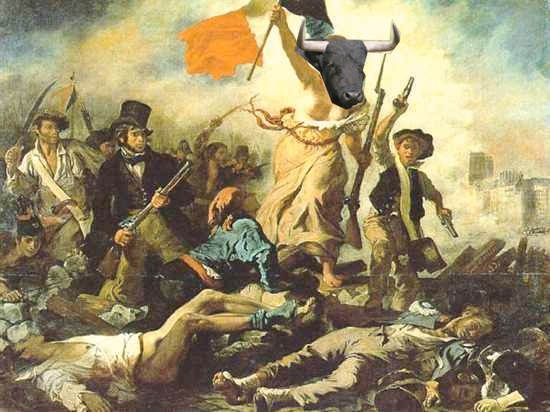
\includegraphics[width=0.5\textwidth]{img/ToroRevolucion.jpg}
\caption{Un toro de revolución.}
\label{figToroRevolucion}
\end{figure}

Pero además, el toro es homeomorfo al producto de dos circunferencias $\mathbb{S}^1 × \mathbb{S}^1$.

\begin{prop} Sea $\appl{f}{\tops}{(ℝ, \topu)}$ continua y \tops compacto. Entonces $f$ alcanza un máximo y un mínimo, es decir, existen $x_+, x_-$ en $X$ tal que $f(x_-) ≤ f(x) ≤ f(x_+)\; ∀x∈X$.
\end{prop}

\begin{proof} Si $f$ es continua y $X$ compacto, entonces $f(X)$ es compacto y tiene un máximo y un mínimo.
\end{proof}

\subsection{Compacidad en términos de cerrados}

En el curso de análisis veíamos, por ejemplo, que si tenemos una sucesión de intervalos cerrados en $ℝ$ en la que cada uno está contenido dentro del anterior, su intersección es no vacía: el supremo de los bordes inferiores y el ínfimo de los superiores tenía que estar en todos. Nos podemos preguntar si esto ocurre por las propiedades especiales de $ℝ$ o lo único que ocurre es que su estructura nos permite hacer la prueba más sencilla. Vamos a verlo. Primero necesitaremos definir una propiedad para intersecciones:

\begin{defn}[Propiedad\IS de intersección finita] Dada una familia de conjuntos $\{A_i\}_{i∈I}$, se dice que tienen la propiedad de intersección finita si su intersección es no vacía para todo subconjunto finito de esa familia, es decir, que \[ \bigcap_{j∈J} A_j ≠ ∅ \quad ∀J⊆I \text{finito} \]

\end{defn}

\begin{prop} Sea \tops un espacio topológico. Son equivalentes
\begin{enumerate}
	\item $X$ es compacto.
	\item Toda familia de cerrados $\{F_i\}_{i∈I}$ con la propiedad de intersección finita tiene intersección no vacía. Es decir, si $\bigcap_{j∈J} F_j ≠  ∅$ para todo subconjunto $J$ de $I$ finito entonces $\bigcap_{i∈I} F_i ≠ ∅$.
	\item Toda familia de cerrados $\{F_i\}_{i∈I}$ tal que $\bigcap_{i∈I} F_i = ∅$ tiene una subfamilia $\{F_j\}_{j∈J}$ con $J⊆I$ finito y $\bigcap_{j∈J}F_j = ∅$.
\end{enumerate}
\end{prop}

\begin{corol} Sea \tops un espacio topológico compacto y $F_1 ⊇ F_2 ⊇ F_3 ⊇ \dotsb$ una sucesión decreciente de cerrados no vacíos. Entonces \[ \bigcap_{n∈ℕ} F_n ≠ ∅\]
\end{corol}

\begin{proof}
Vamos a usar la proposición anterior. Si $J⊆ℕ$ es finito, entonces  \[ \bigcap_{j∈J} F_j = F_m\] donde $m = \max J$, y $F_m ≠∅$ por hipótesis. Es decir, $\{F_n\}_{n∈ℕ}$ cumple la propiedad de la intersección finita y por la equivalencia 2 de la proposición anterior se tiene que \[ \bigcap_{n=1}^∞ F_n ≠ ∅\]
\end{proof}

\subsection{Compacidad en espacios métricos}

\begin{prop} \label{propCompMetrico} Sea \sdst espacio métrico y $\topl_{\dst}$ la topología inducida por la distancia $\dst$. Entonces

\begin{enumerate}
	\item Sea $W⊆X$. Son equivalentes
	\begin{enumerate}
		\item $W$ es compacto.
		\item Todo subconjunto infinito de $W$ tiene un punto de acumulación en $W$.
		\item Toda sucesión en $W$ tiene una subsucesión convergente a un punto de $W$.
	\end{enumerate}
	\item $W⊆X$ compacto implica $W$ cerrado y acotado\footnote{$W$ es acotado si y sólo si $\sup_{x,y∈W} \dst(x,y)$ es finito.}, lo que ocurre si y sólo si $W⊆\bola(a,R)$ para algún $a∈X$, $R>0$.
\end{enumerate}
\end{prop}

\begin{proof}
\begin{enumerate}
	\item Vamos a demostrar primero que \textit{a} implica \textit{b}. Suponemos que $W$ es compacto con puntos de acumulación. Es decir, $W'∩W ≠ ∅$.

	Sea $B⊆W$ infinito, entonces si $B'∩W=∅$ se tiene que $∀w∈W\quad ∃V_w$ abierto tal que $V_w \setminus \set{w} ∩ B = ∅$.

	Sin embargo, como todo $w∈W$ tiene su abierto, entonces $\{V_w\}_{w∈W}$ es un recubrimiento abierto de $W$. Pero por ser $W$ compacto, $∃w_1, \dotsc, w_m$ en $W$ tales que $W ⊆ \bigcup_{k=1}^m W_{w_k}$, luego \[ B ⊆ \bigcup_{k=1}^m V_{w_k} \]

	Podemos restringir eso un poco más de la siguiente forma: \[ B ⊆ \bigcup_{k=1}^m (V_{w_k} ∩ B) ⊆ \{ w_1, \dotsc, w_m\}\], concluyendo entonces que $B$ es finito, contradicción.

	Vamos ahora con la implicación \textit{b} implica \textit{c}. Sea $\{w_n\}$ una sucesión en $W$. Nos preguntamos si existe una sucesión $n_1 < n_2 < n_3$ tal que $W_{n_k} \convs[][k] w ∈ W$. Se pueden dar varios casos.

	Por ejemplo, si el conjunto de valores$\{w_n \tq n ∈ ℕ\}$ es finito existe un $w$ tal que $w_n = w$ para infinitos $n$, y ya tenemos subsucesión.

	Otro caso puede ser que $\{w_n \tq n ∈ ℕ\}$ sea infinito. Por \textit{b}, existe un $w∈W$ tal que $w∈B'$, un punto de acumulación.


	% % Clase de 13-11
	Vamos ahora con: $b\implies c$.	Queremos demostrar que dado $A\subseteq W$ infinito, $A'∩W ≠ ∅$ (esto incluye que $A' ≠ ∅$).

	Sea $B =\set{W_n \tq n∈ℕ}$.

	Caso 1: Si $B$ es finito, no tenemos nada que demostrar porque:

	Caso 2: $B$ infinito

	$$B\quad infinito \underset{hip}{\implies} B'∩ W≠\emptyset, \text{ es decir }, ∃w∈W, w∈B' (\dimplies ∀r>0, \bolac(w,r) ∩ B ≠\emptyset)$$

	¿Existen $n_1<n_2<n_3,... \tq w_{n_k} \to w$? Como estamos en un espacio métrico esto es: $d(w,w_{n_k}) \convs{k\to\infty}{0}$.

	Tomando $r=1$ tenemos $ \bolac(w,r) ∩B≠\emptyset \implies ∃n_1∈ℕ \tq d(w_1,w) < r_1$.

	Sea $d_1 = \min \{d(w,w_n) : n≤ n_1,d w≠w_n\} > 0$ y $r_2 = \min\left\{\frac{1}{2},d_1\right\}$

	Entonces: $\bolac(w,r_2) ∩B ≠ \emptyset ∃ n_2 \tq 0 < d(w_{n_1},w_{n_2}) < r_2$

	Aformación: $n_2 > n_1$.

	Razón: $0 < d(w,w_{n_2}) < r_2 ≤ d_1 = \min d(w_1,w_n)$,

	si $n_2 ≤ n_1$ entonces $0< d(w,w_{n_2}) < d(w,w_{n_2})$ lo que es imposible.

	Por inducción, definimos $d_2 = \min \{d(w,w_n): n≤2, w≠w_n\}$ y $r_3 = \min\left\{\frac{1}{3},d_2\right\}$.

	\textit{Esta demostración hay que arreglarla.}

	\item $W$ compacto $\implies$ cerrado y acotado.

	Demostración:

	1) $(X,d) \overset{\topl_{\dst}}{ \to}$ Hausdorff $\overset{compacto}{\implies} W$ es cerrado.

	2) $\appl{d}{W×W}{ℝ}$ es continua y como $W×W$ es compacto $\implies d$ alcanza un máximo, es decir $∃x_0,y_0 ∈W \tq d(x,y) ≤ d(x_0,y_0) ∀x,y ∈W$.

	Esto implica que el diámetro de $W = \sup d(x,y) ≤ d(x_0,y_0)< \infty$
	\end{enumerate}

\obs $a\implies b $ vale para cualquier espacio topológico $\to$ revisar la demostración ya sólo usa la definición de compacidad.\footnote{What.}

\end{proof}

¿Cuando es cierto que compacto equivale a cerrado y acotado? ¿Que propiedad de un espacio topológico $(X,\dst)$ nos asegura esto?

Cuando en un espacio topológico ocurre esto, diremos que tiene la \concept[Propiedad!Heine-Borel]{propiedad Heine-Borel}. Por ejemplo, ningún espacio métrico incompleto (ahora veremos qué es eso), como $(ℚ, \dst)$ cumple la propiedad. De hecho, incluso espacios métricos completos pueden no tenerla. Vamos a formalizarlo:

\begin{prop} Dado un espacio métrico $(X, \dst)$, se dice que tiene la propiedad Heine-Borel (esto es, cualquier subconjunto cerrado y acotado es compacto) si y sólo si las bolas cerradas \[ \bolac(x,r) = \set{p ∈ X \tq \dst(x,p) ≤ r} \] son compactas.

\end{prop}

\begin{prop} Sea \sdst un espacio métrico con $\topl_{\dst}$ la topología inducida por la distancia, y $W⊆X$. Entonces si $x∈W'$ entonces $\bola(x, r) ∩ W$ es infinito $∀r > 0$.\footnote{No sé qué es esto, que alguien lo explique un poco. También falta la demostración.}
\end{prop}

\begin{defn}[Sucesión\IS de Cauchy] Sea \sdst un espacio métrico. Entonces una sucesión $\{x_n\}$ en $X$ es de Cauchy si y sólo si $∀ε>0\;∃n_ε$ tal que $∀n,m ≥ n_ε$ se tiene que que $\dst(x_n, x_m) < ε$.
\end{defn}

\begin{defn}[Espacio\IS métrico completo] Sea \sdst un espacio métrico. Se dice que es completo si toda sucesión de Cauchy converge.
\end{defn}

Esta noción de convergencia sin necesidad de saber el límite nos viene muy bien para demostrar que existen puntos con cierta propiedad si sabemos cómo aproximarlos a través de una sucesión.

\begin{prop} Si \sdst es un espacio métrico compacto entonces es completo.\end{prop}

\begin{proof} Sea $\{x_n\}$ una sucesión de Cauchy. Por ser $X$ compacto, podemos usar la proposición \ref{propCompMetrico} y entonces sabemos que existe una subsucesión convergente a un punto de $X$. Es decir, $∃x∈X$ y $n_1< n_2 < \dotsb$ tal que $x_{n_k}\convs[][k] x$.

Afirmamos que entonces $x_n \convs x$. Si tomamos $ε>0$, queremos saber si $∃\hat{n_ε}$ tal que $∀n≥n_ε\; \dst(x, x_n) < ε$.

Por tener la subsucesión convergente, sabemos que $∃k_ε$ tal que $∀k≥k_ε\; \dst(x, x_{n_k}) < \frac{ε}{2}$.

Por ser $\{x_n\}$ de Cauchy, podemos encontrar otro $n_ε$ tal que $∀n,m ≥ n_ε\; \dst(x_n, x_m) < \frac{ε}{2}$. Como $n_k$ tiende a infinito, entonces $∃\hat{k}_ε > k_ε\; n_{\hat{k}_ε} ≥ n_ε$. Si $n≥n_ε$ entonces $\dst(x, x_n) ≤ \dst(x, x_{n_{\hat{k}_ε}}) + \dst(x_{n_{\hat{k}_ε}}, x_n) < ε$ y ya tenemos lo que queríamos demostrar.\footnote{Aquí me ha bailado algún subíndice sssssssseguro.}
\end{proof}

¿Para qué nos sirve esto? Veámoslo. Tomemos \sdst un espacio métrico, $K⊆X$ compacto y $x∈K^c$. Entonces \[ \dst(x, K) ≝ \inf\{\dst(x,y) \tq y ∈ K\}\]

En este caso, por ser $K$ compacto, ese ínfimo es un mínimo, es decir, $∃\hat{x} ∈ K$ tal que $\dst(x, K) = \dst(x, \hat{x})$.

¿Por qué? Ya sabemos que $δ = \dst(x,K) = \inf\{\dst(x,y) \tq y ∈ K\}$. Luego $∃y_n∈K$ tal que $\dst(x, y_n) \to δ$. $\{y_n\}$ es una sucesión en $K$, y al ser $K$ compacto existe una subsucesión $\{y_{n_k}\}$ convergente a $y∈K$, y como $\dst(x, y_n) \convs δ$ entonces $\dst(x, y_{n_k}) \convs[][k] δ$, luego $\dst(x, \hat{x}) = δ$.

Como ejercicio sobre este tema, podemos ver que en $ℝ^m$ con la distancia euclídea basta que $K$ sea cerrado para que el ínfimo sea un mínimo.

\begin{prop} En una topología del orden $\topl_<$ de un conjunto $X$, para que los conexos sean los intervalos (y nada más) hacen falta dos propiedades:

\begin{enumerate}
	\item $∀x,y∈X$ con $x<y$, $∃z∈X$ tal que $x<z<y$.
	\item Propiedad del supremo: todo conjunto acotado superiormente tiene un supremo.
\end{enumerate}
\end{prop}

\begin{prop} Sea $(X,<)$ ordenado con orden total y $\topl_<$ la topología del orden. Supongamos que $(X,<)$ tiene la propiedad del supremo. Entonces $∀a,b ∈ X$ el conjunto $[a,b] = \{ x ∈ X \tq a ≤ x ≤ b \} $ es compacto.
\end{prop}

\begin{proof} Empezamos con una observación previa: en un orden sólo puede haber dos tipos de puntos, los que tienen un siguiente o los que no. Más formalmente: si $x∈X$ pueden pasar dos cosas:

\begin{enumerate}
	\item $∃y∈X$ con $y > x$ tal que $(x,y) = ∅$ (no hay puntos entre $x$ e $y$).
	\item $∀y∈X$ con $y > x$, se tiene que $(x,y) ≠ ∅$. Es decir, $∃z∈X$ con $x<z<y$.
\end{enumerate}

Ocurre lo mismo desde la izquierda, con $y<x$.

Para demostrarlo, vamos a ver dos ideas. Sea $\{A_i\}_{i∈I}$ un recubrimiento abierto de $[a,b]$. Entonces, dado $x∈[a,b)$, existe $y_x$ con $x<y_x≤b$ tal que existe un SRF para $
[x, y_x]$.

Encadenando estos intervalos podríamos ir ampliando el subrecubrimiento finito hasta llegar a $[a,b]$, siempre y cuando podamos ampliarlos tanto como para llegar a $b$. Es fácil ver que es imposible que no lleguemos, ya que si sólo llegamos hasta $c$, podemos aplicar de nuevo la misma idea y sacar más intervalos.

Una vez que tenemos la idea, vamos a la demostración formal.

Dado $x∈[a,b)$, $∃y=y_x$ con $x < y ≤ b$ tal que que existe un SRF de $\{A_i\}_{i∈I}$ para $[x,y]$.

Vamos a demostrar esto viendo los dos casos que pueden ocurrir. En el primer caso, $∃y ∈ X$ con $y<x$ y tal que $(x,y) = ∅$. Como $x<b, y ≤ b$, existen $i_x, i_y$ tales que $x∈A_{i_x},\, y∈A_{i_y}$ y entonces el recubrimiento finito para $[x,y] = \{ x,y \}$ es $A_{i_x} ∪ A_{i_y}$, finito.

La otra posibilidad que podemos tener es que no exista tal $y$, es decir, que $∀w ∈ X\; ∃z ∈ X$ con $w > z > x$.

Como $x∈[a,b]⊆\bigcup A_i$, sabemos que $∃i_x$ tal que $x∈A_{i_x}$. Así, $∃β>x$ tal que $[x,β) ⊆ A_{i_x}$. Podemos suponer $β<b$ (si no, tomamos $\min (β, b)$), luego $∃z∈X$ con $x<z<β≤b$. Es decir, $[x, z] ⊆ [x,β) ⊆ A_{i_x}$, y ya hemos encontrado nuestro SRF.

Ahora tenemos que escribir bien en qué consiste lo de ``ampliar por la derecha''. Partimos de que para $x=a$ existe un $y_a$ con $a<y_a<b$ tal que existe un SRF para $[a,y_a]$, y definimos \[ D ≝ \{ y ∈ X \tq y ≤ b \y ∃ \text{ SRF para } [a,y] \}\]

Nuestro objetivo es ver que $b ∈ D$ para encontrar el SRF de todo el intervalo.

Sea $c = \sup D$, que está bien definido por ser $D$ acotado superiormente. Como $y_a∈D$, sabemos que $c > a$.

Proponemos que $c∈D$, y vamos a demostrarlo por reducción al absurdo. Supongamos que $c ∉ D$. Sabemos que $c ≤ b$, así que $∃i_c$ tal que $c ∈ A_{i_c}$.

Por ser $A_{i_c}$ abierto, $∃α < c$ tal que $(α, c] ⊆ A_{i_c}$. No puede ser que $(α,c] ∩ D$ sea vacía, ya que en ese caso $c$ no podría ser el supremo de $D$ pues $c ∉ D$.

Por otra parte, si $(α, c] ∩ D ≠ ∅$ entonces $∃x ∈ D$ tal que $x∈ (α,c] ⊆ A_{i_c}$. Así, $[a,c] ⊆ [a,x] ∪ (α, c]$, y entonces tenemos un SRF para $[a,c]$, luego $c∈D$, contradicción con hipótesis.

Es decir, hemos demostrado que $c∈D$: sólo nos falta demostrar que $c=b$ para encontrar el SRF de $[a,b]$ y demostrar que es compacto.

Si $c < b$, por el primer paso $∃y_c$ con $c < y_c ≤ b$ tal que existe un SRF para $[c, y_c]$, y en ese caso, igual que antes, tendríamos que $[a, y_c] = [a,c] ∪ [c, y_c]$, lo que nos permite encontrar un SRF para $[a,y_c]$, luego $c∈D$, contradicción porque hemos dicho que $y_c > c$.
\end{proof}

\begin{corol} $([0,1] × [0,1], \topl_{Lex})$ es compacto, y también cualquier intervalo cerrado $[a,b]_{Lex}$.\end{corol}

¿Para qué nos sirve esto? Pues para ver cómo demostrar teoremas como el del punto fijo en espacios métricos y no sólo en $ℝ$.

\begin{theorem}[Teorema\IS del punto fijo] Sea \sdst un espacio métrico compacto y $\appl{f}{X}{X}$ una aplicación contractiva, esto es, una aplicación tal que $∃λ < 1$ con \[ \dst(f(x), f(y)) ≤ λ \dst(x,y)\; ∀x,y ∈ X \].

Entonces $f$ tiene un único punto fijo, es decir, $\uexists x_f ∈ X$ tal que $f(x_f) = x_f$.
\end{theorem}

\begin{proof} Demostrar la unicidad es sencillo: si existen $x_1, x_2$ tales que $f(x_1) = x_1,\, f(x_2) = x_2$, tenemos que $\dst(x_1, x_2) = \dst(f(x_1), f(x_2)) ≤ λ \dst(x_1, x_2)$. Luego por ser $λ < 1$, sólo puede ser $\dst(x_1, x_2) = 0$ y entonces $x_1 = x_2$.

Para demostrar la existencia vamos a tener que trabajar algo más. Sea $x_0 ∈ X$. Definimos por recursión una sucesión $x_n$ dada por $x_{n+1} = f(x_n)$ para $n≥ 0$.

Afirmamos que $\{x_n\}$ es sucesión de Cauchy. Sabemos que $\dst(x_n, x_{n+1}) ≤ λ^n \dst(x_0, x_1)$. \footnote{$\dst(x_n, x_{n+1}) ≤ \dst(f(x_n), f(x_{n+1})) ≤ λ \dst(x_{n-1}, x_n) ≤ \dotsb$} Entonces, si $n>m$, \begin{multline*} \dst(x_m, x_n) ≤ \dst (x_m, x_m+1) + \dst(x_{m-1}, x_m) + \dotsb + \dst(x_{n-1}, x_n) ≤ \\ ≤ (λ^m + \dotsb + λ^{n-1}) \dst(x_0, \dst(x_1)) \end{multline*}

Tenemos multiplicando a una suma geométrica, luego \[ \dst(x_m, x_n) ≤ \sum_{k=m}^∞ λ^k \dst(x_0, x_1)\ = \frac{λ^m}{1-λ} \dst(x_0, x_1) \convs[][m] 0 \], así que efectivamente $\{x_n\}$ es de Cauchy.

Por ser $X$ compacto, $X$ es completo y entonces $x_n \convs x$. Pero en ese caso, al tener $x_{n+1} = f(x_n)$ y ser $f$ continua, tenemos que $x= f(x)$.
\end{proof}

Si nos fijamos, en la demostración anterior no hemos usado que $X$ sea compacto: nos basta $X$ completo.

También podemos suavizar las hipótesis un poco en este teorema.

\begin{prop} Sea \sdst un espacio métrico compacto y $\appl{f}{X}{X}$ tal que $\dst(f(x), f(x)) < \dst(x,y)\;∀x,y∈X$ con $x≠y$. Entonces $f$ tiene un punto fijo y es único.
\end{prop}
\begin{proof}
Sea \begin{align*}
\appl{F}{X&}{ℝ} \\
x&\longmapsto \dst(x,f(x))
\end{align*}

que es continua pues $F$ es la composición de funciones continuas.

En ese caso, $F$ continua y $X$ compacto, sabemos que $F$ alcanza un mínimo: $∃x_0 ∈ X$ tal que $F(x) ≥ F(x_0)\; ∀ x∈X$.

Afirmamos que $\dst(x_0, f(x_0)) = F(x_0) = 0$. Sea $y_0 = f(x_0)$. Si $x_0 ≠ y_0$, tenemos que, por hipótesis, \[ \dst(y_0, f(y_0)) < \dst(x_0, y_0) = \dst(x_0, f(x_0)) \],
 es decir, $F(y_0) < F(x_0) = \min F$, contradicción. Por lo tanto $x_0 = y_0 = f(x_0)$, luego ya tenemos nuestro punto fijo.

La unicidad se deja como ejercicio para el lector.
\end{proof}

Un comentario: para este resultado, con una hipótesis más débil, no es cierto para espacios métricos completos en general. Por ejemplo, si tomamos \[ f(x) = x - \arctan x - \frac{π}{2}\], en el espacio métrico completo (pero no compacto) $(ℝ. \dst)$ con la distancia habitual, no tiene punto fijo. Si lo tuviese, se debería cumplir $\arctan x = - \frac{π}{2}$, que no tiene solución ($x$ debería ser infinito). Sin embargo, sí cumple la hipótesis \[ \abs{f(x) - f(y)} < \abs{x -y}\quad x≠y \], pues $\abs{f'(t)} < 1 \; ∀t ∈ ℝ$.

\begin{prop} La compacidad es una propiedad topológica. Esto es, si $X$ e $Y$ son homeomorfos y $X$ es compacto, entonces $Y$ es compacto. \end{prop}

\section{Axiomas de numerabilidad}

\begin{defn}[Base\IS de entornos] Sea \stopl un espacio topológico, y $x∈X$. Sea $\mathcal{V} = \{V_i\}_{i∈I⊆ℕ}$ con $V_i ⊆ X$. Se dice que $\mathcal{V}$ es una base de entornos de $x$ si y sólo si \begin{enumerate}
	\item Todos los entornos son abiertos en la topología: $V_i ∈ \topl\; ∀i∈I$.
	\item Todos los conjuntos son entornos de $x$: $x∈V_i \; ∀i ∈ I$.
	\item Cualquier abierto de la topología que contenga a $x$ tiene que contener también algún entorno de la base:

	\[ ∀A ∈ \topl \tq x∈ A,\; ∃i = i_A \tq V_i ⊆ A\]
\end{enumerate}\label{defBaseEntornos}
\end{defn}

\begin{defn}[Axioma\IS de numerabilidad I] Sea \stopl un espacio topológico. Se dice que es primer axioma de numerabilidad (IAN) si y sólo si todo punto $x∈X$ tiene una base de entornos numerable. Es decir, que existen $\{V_x^n\}_{n∈ℕ}$ entornos de $x$ tales que $∀A$ abierto con $x∈A$ existe un $n=n_A$ tal que $x∈V_x^n ⊆ A$
\end{defn}

Un comentario: tomando $\hat{V}_x^n = V_x^1 ∩  V_x^2 ∩ \dotsb ∩ V_x^n$ (que también es entorno de $x$) se puede suponer una sucesión decreciente de entornos $\hat{V}_x^1 ⊇ \hat{V}_x^2 ⊇ \dotsb$.

Lo que se intenta ``imitar'' con esta noción son las bolas de centro $x$ y radio $\frac{1}{n}$ en un espacio métrico, y así demostrar propiedades de espacios métricos sin necesidad de tener una distancia.

\begin{defn}[Axioma\IS de numerablidad II] Sea \stopl un espacio topológico. Se dice que $X$ es segundo axioma de numerabilidad (IIAN) si y sólo si existe una base numerable o finita para la topología. Es decir, si $∃\base = \{ B_n\}_{n∈ℕ}$ con $\topl = \topl_\base$.
\end{defn}

Un ejemplo sencillo es $ℝ$ con la topología usual. Podemos encontrar una base numerable \[ \base = \{ (a,b) \tq a,b ∈ ℚ,\, a<b\}\] y a partir de ella construir cualquier intervalo.

\begin{defn}[Espacio\IS separable] Sea \stopl un espacio topológico. Entonces se dice que es separable si y sólo si existe un subconjunto numerable o finito que es denso en $X$. Es decir, que $∃D⊆X$ tal que $\card{D} ≤ \card{N}$ y tal que $\adh{D} = X$. \label{defEspacioSeparable}
\end{defn}

Más ejemplos familiares: en $ℝ$ con la topología usual, podemos tomar $D=ℚ$ que es numerable y $\adh{ℚ} = ℝ$.

\begin{prop} Sea \stopl un espacio topológico. Entonces \begin{enumerate}
	\item Si $X$ es IIAN entonces es IAN y separable.
	\item Si $X$ es IAN y $W⊆X$ entonces \begin{enumerate}
		\item $x∈\adh{W}$ si y sólo si existe una sucesión $\{x_n\} ⊆ W$ tal que $x_n \to x$. Es lo que se llama \concept[Caracterización por sucesiones! de la adherencia]{caracterización por sucesiones\IS de la adherencia}.
		\item Si $W$ es compacto, toda sucesión en $W$ tiene una subsucesión convergente a un punto de $W$.
	\end{enumerate}
\end{enumerate}
\end{prop}

Si nos fijamos, son propiedades que ya hemos demostrado para espacios métricos usando esas bolas de radio $\frac{1}{n}$. Vamos a por la demostración.

\begin{proof}
\begin{enumerate}
	\item Por hipótesis, sabemos que $\topl = \topl_\base$ con $\base = \{ B_n\}_{n∈ℕ}$.

	Para demostrar que es IAN, sea $x∈X$ y tomamos los $B_n ∈ \base$ tales que $x∈B_n$. Son, a lo más, una cantidad numerable y son base de entornos, pues por definición de $\topl_\base$ sabemos que $x∈A$ abierto si y sólo si $∃B∈\base$ tal que $x∈B_n ⊆ A$.

	Para la separabilidad, sea $x_n ∈ B_n$ (suponemos todos los $B_n ≠ ∅$). Entonces \[ D = \{ x_n \tq n ∈ ℕ\}\] es numerable y $\adh{D} = X$, ya que $∀x∈X$ y $∀A ∈ \topl$ con $x∈A$, existe un $B_m ∈ \base$ con $x∈B_m ⊆ A$, luego $x_m ∈ A∩D ⊇ B_m ∩ D ≠ ∅$, luego $x∈\adh{D}$ y entonces es el total.
	\item Como en espacios métricos. Se deja como ejercicio para el lector.
\end{enumerate}
\end{proof}

\section{Axiomas de separación}

Hausdorff (ver \ref{defHausdorff}) es un axioma de separación.

\begin{defn}[Espacio\IS regular] Sea \stopl espacio topológico. Se dice que es regular si y sólo si $∀x∈X$ y $∀C⊆X$ cerrado y tal que $x∉C$ existen $A, B$ abiertos y disjuntos y tales que $x∈A,\, C⊆B$.
\end{defn}

\begin{defn}[Espacio\IS normal] Sea $\stopl$ un espacio topológico. Se dice que es normal si y sólo si dos cerrados disjuntos se pueden separar. Es decir, que si $C_1, C_2$ son cerrados con $C_1 ∩ C_2 = ∅$,, entonces existen abiertos $A_1, A_2$ tales que $C_j ⊆ A_j,\, j=1,2$ y $A_1 ∩ A_2 = ∅$.
\end{defn}

Es fácil ver que hemos ido ``subiendo'' en requisitos. Con Hausdorff pedimos separar dos puntos, con regularidad separamos un punto y un conjunto y con la normalidad separamos directamente conjuntos.

A partir de aquí podemos caracterizar por los $T_x$. Se dice que un espacio topológico \stopl es \begin{enumerate}
	\item $T_2$ si y sólo si es Hausdorff.
	\item $T_3$ si y sólo si es Hausdorff y regular.
	\item $T_4$ si y sólo si es Hausdorff, regular y normal.
\end{enumerate}

\begin{prop} Varias equivalencias con las definiciones anteriores:
\begin{enumerate}
	\item $T_4 \implies T_3 \implies T_2$. Como idea, en un $T_2$, $\{x\}$ es cerrado $∀x∈X$.
	\item Un espacio compacto y Hausdorff es $T_4$.
\end{enumerate}
\end{prop}

\begin{proof}
\begin{enumerate}
	\item
	\item Para $T_3$, una idea: podemos coger para cada punto $x∈C$ un entorno suyo y un entorno de $x$. Como estamos en compactos, podemos coger algo.\footnote{Aquí habría que copiarlo y explicarlo bien.}
\end{enumerate}
\end{proof}

Un ejemplo: vamos a ver si $(ℝ, \topl_{[,)})$ es IAN, IIAN y separable. Para ver si es IAN, vemos que para todo $x∈ℝ$ podemos coger entornos $V_x^n = [x, x + \frac{1}{n})$ abiertos. Además, si $A∈\topl_{[,)}$ y $x∈A$, tenemos que $∃δ$ tal que $[x, x+δ) ⊆ A$ tomando un entorno $V_x^n$ tal que $\frac{1}{n} < δ$.

Vamos ahora a ver si si es IIAN. Para podes escribir $[b,c) = \bigcup_{i∈I} [b_i, c_i)$ con $I$ no necesariamente numerable, $∃i$ tal que $b = b_i$. Luego si $\base$ es una base para $\topl_{[,)}$, entonces $∀x∈ℝ$ tiene que existir un $B_x ∈ \base$ tal que $x∈B_x$ y con $(-∞, x) ∩ B_x = ∅$. Afirmamos\footnote{Y lo dejamos como ejercicio.} que los $B_x$ son todos distintos, y entonces $\card{\base} ≥ \card{ℝ}$.

Por último, sabemos que es separable porque tenemos que $ℚ$ es denso.

\seprule

Esto va en alguna parte.

Ejemplo de que $\dst(x,F)$ puede no alcanzarse si sólo se pide $F$ cerrado. Es decir, que puede no existir $y_0 ∈ F$ tal que $\dst(x,y_0) ≤ \dst(x,y)\; ∀y∈F$.

Tomamos, por ejemplo, $X = l^2$, el espacio de sucesiones $\{x_n\}_{n=1}^∞$ tales que $\sum x_n^2 < ∞$, con la siguiente distancia: \[ \dst(x,y) = \sqrt{\sum_{n=1}^∞ \abs{x_n - y_n}^2 }\] y tomamos el conjunto $F$ como  \[ F = \left\{ y ∈ l^2 \tq ∃m∈ℕ \text{ con } \begin{matrix} y_n &=& 0 & n ≠ m \\ y_m & = & 1 + \frac{1}{m} & \end{matrix}\right\} \]

Tenemos que para $y∈F$, $\dst(0,y) = 1 + \frac{1}{m}$, cuyo ínfimo es $1$, luego $\dst(0, F) = 1$, sin embargo $\dst(0,y) > 1$ $∀y∈F$. Sólo faltaría demostrar que $F$ es cerrado, y se deja como ejercicio.

\chapter{Conceptos básicos de homotopía}

\section{Homotopía de caminos}

\begin{defn}[Función\IS homotópica] Sean $X, Y$ espacios topológicos y $\appl{f_0,f_1}{X}{Y}$ continuas. Se dice que $f_0, f_1$ son homotópicas si y sólo si existe una aplicación $\appl{F}{[0,1]×X}{Y}$ continua (tomando la topología producto) tal que \[ F(0,x) = f_0(x), \, F(1,x) = f_1(x)\]

Entonces se dice que $F$ es una homotopía entre $f_0$ y $f_1$.
\end{defn}

\begin{figure}[hbtp]
\inputtikz{III_Deformacion}
\caption{Deformación continua de dos funciones}
\end{figure}

Tenemos que $f_t(x) = F(t,x)$, y que $\appl{f_t}{X}{Y}$ es continua. Por tanto, una construcción del tipo

\[x \to (t,x) \to Y\]

(donde la segunda aplicación es $F$) es equivalente a $f_t$ que es continua. Y por tanto la primera aplicación también debe serlo, pues $F$ también es continua.

De la $f_t$ decimos que es una deformación continua de $f_0$ a $f_1$.

\begin{figure}[hbtp]
\inputtikz{III_Homotopicas_caminos}
\caption{Funciones homotópicas por caminos}
\label{figHomotopicaCaminos}
\end{figure}

\begin{defn}[Función\IS homotópica por caminos] Sea $X$ un espacio topológico y $\appl{f_0,f_1}{[0,1]}{X}$ aplicaciones continuas y tales que:

\begin{align*}
f_0(0) &= f_1(0) = x_0 \\
f_0(1) &= f_1(1) = x_1
\end{align*}

Entonces. se dice que $f_1$ y $f_2$ son homotópicas por caminos si y sólo si $∃ \appl{F}{[0,1]×[0,1]}{X}$ continua tal que
\[F(0,s)=f_0(s), \, F(1,s)=f_1(s); \quad ∀s∈[0,1]\]

y además
\[ F(t,0)=x_0 , \, F(t,1)=x_1 \quad ∀t∈[0,1]\]

Es decir, que $F$ parte de $f_0$ y lleva a $f_1$ si movemos el parámetro $s$, y siempre nos lleva de $x_0$ a $x_1$ moviendo el parámetro $t$.
\end{defn}

Como notación más sencilla, consideraremos $f_t(s) = F(t,s)$, donde también se cumple que $f_t(0)=x_0$, $f_t(1)=x_1$.

Para denotar que existe esta función $F$, diremos que $f_0 \dfm f_1$ (la `p' viene de \textit{path}).

\begin{example}
\begin{figure}[hbtp]
\inputtikz{III_Deformacion_convexo}
\caption{Deformaciones continuas en un espacio convexo.}
\label{figDefmConvexo}
\end{figure}

Tomamos $X⊆ℝ^m$, convexo, y $\appl{f_0,f_1}{[0,1]}{X}$, que son caminos continuos con $f_0(0)=f_1(0)=x_0$ y $f_0(1)=f_1(1) = x_1$.

Lo que vamos a hacer para deformar $f_0$ hasta $f_1$, es (ver figura \ref{figDefmConvexo}) trazar los segmentos que unen los puntos de ambos caminos (dichos segmentos se quedan en $X$, porque hemos dicho que es convexo), y vamos pasando por todos los puntos de los segmentos. Entonces \[F(t,s) = tf_1(s) + (1-t)f_0(s); \ 0≤t≤1 \] es continua y cumple las condiciones que necesitamos.

\end{example}


\begin{example}

\begin{figure}[hbtp]
\inputtikz{III_Deformar_imposible}
\caption{Es imposble encontrar una deformación continua de $f_0$ a $f_1$.}
\label{figDefmImposible}
\end{figure}

Tomamos la corona $X = \{(x,y) ∈ ℝ : \ x^2+y^2≥1\}$ y fijándonos en el dibujo (figura \ref{figDefmImposible}) podemos apreciar que $f_0 \not\simeq_p f_1$, puesto que no podemos ``deformar'' $f_0$ para convertirlo en el camino $f_1$ sin pasar por el círculo interior. Este problema se debe a que tenemos los 2 puntos fijos.
\end{example}


\begin{lemma} Sea $\appl{f}{[0,1]}{X}$ continua, $\appl{h}{[0,1]}{[0,1]}$ continua, biyectiva y creciente y $\appl{\hat{f} = f \ast h}{[0,1]}{X}$ continua.

Entonces $f \dfm \hat{f}$.
\end{lemma}

\begin{proof}

$F(t,s) = f(t·h(s) + (1-t) s)$ continua

$t = 0 \to f(s)$

$t = 1 \to f(h(s)) = \hat{f}(s)$

$F(t,0) = f(t·0 + (1-t)·0) = f_0$

e igual con 1

(podemos asegurar lo anterior debido a que como $h$ es biyectiva y creciente, $h(0) = 0$ y $h(1) = 1$)

\obs basta $\appl{h}{[0,1]}{[0,1]}$ continua y tal que $h(0)=0$, $h(1)=1$
\end{proof}


Vamos a introducir una notación para los caminos en $X$ entre dos puntos: \[ C(X, x_0, x_1) = \{ \appl{f}{[0,1]}{X} \text{ continua } \tq f(0) = x_0, f(1) = x_1 \}\]

\begin{prop} $\simeq_p$ es una relación de equivalencia en $C(X, x_0, x_1)$.
\end{prop}

\begin{proof}
Vamos a demostrar las propiedades de relación de equivalencia:

\begin{enumerate}
	\item $f\dfm f$ trivialmente.
	\item $f \dfm g \implies g \dfm f$. La transformación es fácil de ver, cogiendo $\hat{F}(t, s) = F(1-t, s)$.
	\item $f \dfm g, g \dfm h \implies f \dfm h$. Tenemos las transformaciones $F_1$ y $F_2$ respectivamente, y queremos encontrar la que nos lleva de $f$ a $h$. La podemos definir ``acelerando'' las transformaciones y juntándolas:

	\[F(t,s) =
	\begin{cases}
		F_1(2t, s) & 0 ≤ t ≤ \frac{1}{2}, s∈[0,1] \\
		F_2(2t-1, s) & \frac{1}{2} ≤ t ≤ 1, s∈[0,1]
	\end{cases} \]

	Se puede ver que $F$ es continua.
\end{enumerate}
\end{proof}

En la demostración anterior hemos visto fácilmente que $F$ es continua, pero vamos a definir un lema que usaremos más tarde para formalizarlo.

\begin{lemma} \label{lemContRestr} Sean $Y,Z$ espacios topológicos, sea $\appl{f}{Y}{Z}$ y sean $A,B$ cerrados en $Y$ tales que $A ∪ B = Y$ y las restricciones $f|_A, f|_B$ son continuas.

Entonces $f$ es continua
\end{lemma}

\begin{proof} Si $f$ es continua, es lo mismo que decir que la imagen inversa de un cerrado es cerrado. Entonces si $C$ es cerrado en $Z$, $\inv{C}$ se puede escribir de la siguiente forma:

\[ \inv{C}  = \inv{\left(f|_A\right)} ( C) ∪ \inv{\left(f|_B\right)} (C)  \]

Ahora, $\inv{\left(f|_A\right)} ( C)$ es cerrado en $A$ por ser $\restr{f}{A}$ cerrado en $Y$. Ocurre lo mismo para $B$, así que $\inv{f}(C)$ es unión finita de cerrados y entonces $\inv{f}{C}$ es cerrado en $Y$, y entonces $f$ es continua.
\end{proof}

Es fácil ver que esta demostración vale igualmente si $A,B$ son abiertos, simplemente cambiando ``abierto'' por ``cerrado'' en enunciado y demostración.

Vamos ahora a ver varias notaciones.

\begin{defn} Sea $X$ un espacio topológico. Entonces
\begin{enumerate}
	\item Dado $x∈X$, definimos el \concept[Camino\IS constante]{camino\IS constante} $δ_x$ como
	\begin{align*}
	\appl{δ_x}{[0,1]&}{X} \\
	s&\longmapsto δ_x(s) \equiv x
	\end{align*}
	\item Dada $f∈C(X, x_0, x_f)$ se define el \concept[Camino\IS inverso]{camino\IS inverso} \[ f^-(s) = f(1-s) \], que también está en $f∈C(X, x_0, x_f)$.
	\item Dadas $f∈C(X, x_0, x_1),\, g∈C(X, x_1, x_2)$, definimos el \concept[Camino\IS producto]{camino producto} (o concatenación de caminos) como

	\[ f\ast g (s) = \begin{cases}
		f(2s) & 0 ≤ s ≤ \frac{1}{2} \\
		g(2s - 1) & \frac{1}{2} ≤ s ≤ 1
	\end{cases} \]

	Es fácil ver que $f \ast g ∈ C(X, x_0, x_2)$ por el lema anterior que hemos visto.
\end{enumerate}
\end{defn}

\begin{prop} \label{propOpDfm} Sea $X$ un espacio topológico. Entonces
\begin{enumerate}
	\item $f_0 \dfm f_1, g_0 \dfm g_1 \implies f_0 \ast g_0 \dfm f_1 \ast g_1$.
	\item El camino constante es la ``identidad'', por así decirlo, de la operación $\ast$: \[f∈C(X, x_0, x_1) \implies δ_{x_0} \ast f \dfm f, f \ast δ_{x_1} \dfm f \]
	\item La concatenación de un camino con su inverso se puede deformar continuamente en el camino constante en el punto de inicio: \[ f\ast f^- \dfm δ_{x_0},\quad f^- \ast f \dfm δ_{x_1} \] para $f∈C(X, x_0, x_1)$.
	\item La operación producto es asociativa: \[ (f\ast g) \ast h \dfm f \ast (g\ast h) \]
\end{enumerate}
\end{prop}

Suponemos que siempre que consideramos $f\ast g$ se entiende que $f(1) = g(0)$, porque si no no tendría sentido.

\begin{proof}
\begin{enumerate}
	\item Tenemos que $f_0 \dfm f_1$ y $g_0 \dfm g_1$ con las transformaciones $F$ y $G$ respectivamente. Queremos comprobar que existe una transformación $H$ para $f_0 \ast g_0 \dfm f_1 \ast g_1$. Podemos definirla de la siguiente forma:

	\[ H(t,s) = \begin{cases} F(t, 2s) & 0 ≤ s ≤ \frac{1}{2} \\ G(t, 2s-1) & \frac{1}{2} ≤ s ≤ 1 \end{cases} \]

	que es continua por el lema \ref{lemContRestr}. En este caso,

	\[ H(0,s) = \left\{\begin{matrix} F(0,2s) = f_0(2s) & 0 ≤ s ≤ \frac{1}{2} \\
	G(0, 2s-1) = g_0(2s -1) & \frac{1}{2} ≤ s ≤ 1 \end{matrix}\right\} ≝ f_0 \ast y_0(s) \] e igualmente $H(1, s) = f_1 \ast g_1 (s)$.

	Dicho de otra forma, $H(t,s) = f_t \ast g_t (s)$.

	\item Queremos ver que $δ_{x_0} \ast f \dfm f$. Entonces podemos definir la aplicación muy fácilmente de forma visual. Formalmente es un poco peñazo:

	\[ F(t,s) = \begin{cases}
	x_0 & s ≤ \frac{1}{2}(1-t) \\
	f\left(\frac{s-a_t}{1-a_t}\right) & \frac{1}{2}(1-t) = a_t ≤ s ≤ 1 \end{cases}\]

	\item Visualmente también es sencillo. Lo que hacemos es ``ir y volver'', y al ir aumentando la $t$ de la transformación vamos cada vez más cerca del punto de inicio. La transformación sería

	\[ F(t, s) = \begin{cases}
		f((1-t) s ) &  \\
		f^-(ts) & \end{cases} \]

	\item Es facilillo, luego vemos la formulita.
\end{enumerate}
\end{proof}

\subsection{Grupo fundamental}

Vamos a usar algo de notación. Primero, denotaremos el camino en $X$ que sale y lleva del mismo punto por \[ C(X, x_0) \equiv C(X, x_0, x_0) \]

También veremos el conjunto cociente de las clases de equivalencia como \[ π(X, x_0) \equiv \quot{C(X, x_0)}{\dfm} \]

Como recordatorio, dos clases de equivalencia son la misma si se puede transformar el representante del uno en el del otro:

\[ [φ] \equiv [ψ] \iff φ \dfm ψ \]

\begin{prop}

\begin{enumerate}
	\item Dados $[φ], [ψ] ∈ π(X, x_0)$, la operación \[ [φ]\ast [ψ] ≝ [φ\ast ψ]\] está bien definida en $π(X, x_0)$, es decir, no depende de los representantes elegidos.

	\item $\left(π(X, x_0), \ast\right)$ es un grupo. De hecho, le llamaremos el \concept[Grupo\IS fundamental]{grupo fundamental}\footnote{Sólo tiene sentido hablar de grupo fundamental en espacios cpc.} de $X$ con base en $x_0$.
\end{enumerate}
\end{prop}

\begin{proof}
Hay que demostrar que si $[φ] = [\tilde{φ}]$ y $[ψ] = [\tilde{ψ}]$, entonces $[φ\ast ψ] = [\tilde{φ} \ast \tilde{ψ}]$. Sabiendo que $φ \dfm \tilde{φ}$ y $ψ \dfm \tilde{ψ}$, usando la proposición \ref{propOpDfm} entonces $φ\ast ψ \dfm \tilde{φ} \ast \tilde{ψ}$ y por lo tanto \[ [φ\ast ψ] = [\tilde{φ} \ast \tilde{ψ} ] \]

También tenemos que demostrar que ese conjunto con la operación $\ast$ es un grupo. Es claro que el neutro o identidad será el camino constante, $[δ_{x_0}]$, si usamos lo que vimos en la proposición \ref{propOpDfm}.

Para el elemento inverso, dado un $[φ]$ su inverso será $[φ^-]$, ya que \[ [φ^-] \ast [φ] = [φ^- \ast φ] = [δ_{x_0}]\] usando de nuevo la proposición \ref{propOpDfm}. Es decir, $\inv{[φ]} = [φ^-]$.

Lo único que nos falta probar es la propiedad asociativa, y adivinad qué proposición hay que mirar para verlo.
\end{proof}

\begin{prop} Sea $X$ un espacio topológico y $\appl{f}{[0,1]}{X}$ una función continua. Sean $f(0) = x_0, f(1) = x_1$. Entonces sea \[ \hat{f}\left([ψ]\right) ≝ \left[f^- * ψ \ast f\right]\]

La aplicación $\appl{\hat{f}}{π(X, x_0)}{π(X, x_1)}$ está bien definida y es un isomorfismo de grupos.

\end{prop}

\begin{figure}[hbtp]
\centering
\inputtikz{III_IsomorfismoGrupoCaminos}
\caption{Isomorfismo entre caminos.}
\label{figIsomorfismoCaminos}
\end{figure}

\begin{proof} Lo primero es ver qué estamos haciendo. Hay que demostrar que la aplicación no depende del representante. Pero sabemos que $φ\dfm ψ$ implica que $f^- * φ * f \dfm f^- * ψ * f$ por la proposición \ref{propOpDfm} de nuevo.
\end{proof}

\begin{corol} Si $X$ es cpc entonces $π(X, x_0)$ es isomorfo a $π(X, x_1)$ $∀x_0, x_1 ∈ X$. En ese caso se usa $π(X)$ para referirse a uno cualquiera de ellos.
\end{corol}

La razón de este corolario es simple: si es cpc (\ref{defCPC}) podemos encontrar una aplicación continua que nos lleva de $x_0$ a $x_1$, y ya podemos aplicar la proposición.

A partir de ahora y salvo que se diga lo contrario, supondremos que los $X$ son conexos por caminos. Si no, siempre se pueden tomar las componentes cpc.

Vamos a ver varios ejemplos, y empezamos por lo sencillo.  Dado $ℝ^2$, que es cpc, entonces $π(X)$ es\footnote{No es muy matemático esto, un poco de abuso de notación pero se entiende.} el grupo trivial, es decir, $π(X)= \{ 1\}$.

La razón es que, al ser $ℝ^2$ convexo, cualquier aplicación $\appl{φ}{[0,1]}{X}$ continua con $φ(0) = φ(1) = (0,0)$ es deformable al camino constante: $φ \dfm δ_{(0,0)}$ ya que no hay ningún ``agujero'' que nos pare a la hora de deformar.

\begin{defn}[Espacio\IS simplemente conexo] Dado $X$ cpc, se dice que es simplemente conexo si y sólo si $π(X) = \{1\}$, el grupo trivial. Es decir, si todo camino cerrado en $X$ se puede deformar a un punto.\end{defn}


Vamos a ver algunos ejemplos, no demasiado rigurosos.

\begin{enumerate}
\item $\mathbb{S}^1$, la circunferencia de radio $1$. Por comodidad, vamos a usar notación compleja y entonces el camino $φ$ es \[ φ(s) = e^{2πis}\; s∈[0,1]\] (dicho de otra forma, $φ(s) = (\cos 2πs, \sin 2πs)$).

Tomamos el grupo $a = [φ]$, que no es el camino constante $[δ_{(1,0)}]$. Con este grupo podemos operar: $a^n = [φ*φ*φ\dotsb *φ]$, que no es más que dar $n$ vueltas a $\mathbb{S}^1$.  De la misma forma, $a^{-n} = [ φ^- * \dotsb * φ^- ]$, que es dar $n$ vueltas en sentido contrario. Veremos que $π(\mathbb{S}^1)$ es isomorfo a $ℤ$. No lo demostramos, pero es fácil ver que puede existir una aplicación biyectiva

\begin{align*}
ℤ &\longmapsto π(\mathbb{S}^1, (0,1)) \\
n &\longmapsto a^n
\end{align*}

\item Un ejemplo interesante es ver el plano sin un punto: $ℝ^2 \setminus \{ p\}$. En la figura \ref{figCaminosPlano} podemos ver tres tipos de caminos: $α, ψ, φ$. Es fácil ver que $φ$ y $α$ pertenecen al mismogrupo ($φ \dfm α$). En el caso de $ψ$, lo que hace es dar ``dos vueltas'', así que en realidad $ψ \dfm α^2$ o, dicho de otra forma, $[ψ] = [α^2]$.

\begin{figure}[hbtp]
\centering
\inputtikz{III_CaminosPlanoSinPunto}
\caption{Caminos posibles en el plano $ℝ^2 \setminus \{p\}$.}
\label{figCaminosPlano}
\end{figure}

\item El caso del toro $\mathbb{T}^2$ es también curioso porque nos habla de conmutadores o algo así pero no me ha dado tiempo a copiarlo.

\end{enumerate}

Como decíamos antes, esto no es muy riguroso, así que vamos a empezar con los formalismos.

\begin{defn} Sean $X,Y$ espacios topológicos, $x_0∈X, y_0∈Y$. Como notación, la aplicación \[ \appl{f}{(X, x_0)}{(Y, y_0)}\] la tomaremos como $\appl{f}{X}{Y}$ continua con $f(x_0) = y_0$.

Para funciones como $f$, se define $f_\#$ como \[ \appl{f_\#}{π(X, x_0)}{π(Y, y_0)}\] por \[ f_\#([φ]) = [f\circ φ]\]
\end{defn}

\begin{prop} Sea $\appl{f}{(X, x_0)}{(Y, y_0)}$. Entonces
\begin{enumerate}
 	\item $f_\#$ está bien definida y es un homomorfismo de grupos.
 	\item Si $\appl{g}{(X, x_0)}{(Z, z_0)}$ entonces $\left(g○f\right)_\# = g_\# ○ f_\#$.
 	\item Si $\appl{I}{(X, x_0)}{(X, x_0)}$ es la identidad entonces $\appl{I_\#}{π(X, x_0)}{π(X, x_0)}$ es la identidad.
 \end{enumerate}
 \end{prop}

\begin{proof}
\begin{enumerate}
	\item Para ver que está bien definida hay que ver que no dependa de los representantes elegidos.\footnote{Aquí falta algo que no sé qué es.} Si $φ_1 \dfm φ_2$, entonces tenemos que ver que $f○φ_1 \dfm f○φ_2$. Es decir, que si $[φ_1] = [φ_2]$ entonces $[f○φ_1] = [f○φ_2]$. Y esto es cierto, ya que si $φ_1 \dfm φ_2$, entonces existe una aplicación \[ \appl{F}{[0,1]×[0,1]}{X}\] tal que $F(0,s) = φ_1$ y $F(1,s) = φ_2$ y $F(t,0) = F(t,1) = x_0$.

	Sea $H(t,s) = f(F(t,s))$. Entonces es continua por ser composición de continuas y $H(0,s) = f○φ_1(s)$, $H(1,s) = f○φ_2(s)$ y listos.

	Vamos a demostrar ahora que es un homomorfismo de grupos, con las tres propiedades que tocan. Pero es mucho a escribir y realmente no es difícil de ver, así que si alguien quiere que lo copie.

	\item Queremos demostrar ahora que $(g○f)_\#  = g_\# ○ f_\#$. Operando

	\[ (g○f)_\# ([φ]) ≝ [g○f○φ] ≝ g_\#([f○φ]) ≝ g_\#(f_\#([φ])) \]

	y entonces $(g○f)_\# = g_\# ○ f_\#$.

	\item Trivial.
\end{enumerate}
\end{proof}

¿Y para qué queríamos todo esto? Pues para poder demostrar el siguiente corolario: los grupos fundamentales de espacios homeomorfos son isomorfos.

\begin{corol} Sean $X$, $Y$ espacios topológicos cpc y homemorfos uno al otro. Entonces \[ π(X) \simeq π(Y) \]
\end{corol}

\begin{proof} Si $X,Y$ son homeomorfos, entonces $∃\appl{h}{X}{Y}$ continua, biyectiva y con $\inv{h}$ continua.

Sea $x_0 ∈ X,\, y_0 = h(x_0)$. Usando las propiedades anteriores, tenemos que

\[ id_\# = (\inv{h} ○ h)_\# = \inv{h}_\# ○ h_\# \]

y entonces tenemos dos homomorfismos
\begin{align*}
\appl{h_\#}{π(X, x_0)&}{π(Y, y_0)} \\
\appl{\inv{h}_\#}{π(Y, y_0)&}{π(X, x_0)}
\end{align*}

Como su composición es la identidad, entonces $h_\#$ tiene inversa y es entonces un isomorfismo.
\end{proof}

Un uso sencillo de lo que acabamos de ver es estudiar, por ejemplo, el grupo fundamental de la circunferencia en el plano. Las clases de equivalencia son las vueltas que damos: si no damos una vuelta completa (por ejemplo, recorremos sólo media circunferencia), es como no diésemos ninguna, ya que podemos deformarlo a un punto. De la misma forma, si damos dos vueltas no hay forma de deformarlo para dar sólo una.

\begin{prop} \[ π(\mathbb{S}^1) \simeq (ℤ, +)\]

Es decir, $π(\mathbb{S}^1)$ es un grupo cíclico infinito con generador \[ a = [(\cos 2πs, \sin 2πs)]\] y con la siguiente aplicación para llevar de uno a otro:
\begin{align*}
(ℤ, +) &\longmapsto π(\mathbb{S}^1, (1,0)) \\
n &\longmapsto a^n
\end{align*}
\end{prop}

\subsubsection{Construcción de grupos fundamentales}

Ahora vamos a ver cómo construir grupos fundamentales a partir de otros.

\begin{prop} El grupo fundamental del producto es isomorfo al producto de grupos fundamentales:

\[ π(X_1 × X_2) \simeq π(X_1) × π(X_2)\]

siendo ``$×$'' el producto de grupos usual, esto es, con la operación $(a_1, a_2) · (b_1, b_2) = (a_1 · b_1, a_2 · b_2)$.
\end{prop}

\begin{proof}
Si $X_1, X_2$ son cpc, entonces $X_1×X_2$ también lo es. También sabemos que si tenemos una aplicación \[ \appl{φ}{[0,1]}{X_1×X_2}\] continua entonces tienen que ser sus componentes $φ_1, φ_2$ continuas.

Más: si $(φ_1, φ_2) = φ\dfm ψ = (ψ_1, ψ_2)$, entonces tiene que ser $φ_1\dfm ψ_1$ y $φ_2 \dfm ψ_2$. \footnote{Ha llenado media pizarra en un segundo y a partir de aquí no sé qué escribo.}

Entonces si tenemos una deformación \[ \appl{F}{[0,1]×[0,1]}{X_1×X_2}\] continua, se cumple que $φ\dfm ψ$ por $F$ si y sólo si $φ_1\dfm ψ_1$, $φ_2\dfm ψ_2$ por $F_1$ y $F_2$ respectivamente.  Así, por último,

\[ φ*ψ = (φ_1*ψ_1, φ_2*ψ_2)\]
\end{proof}

Ejemplo sencillo de esto, algo que ya habíamos demostrardo: $\mathbb{T}^2$ (el toro) es homeomorfo a $\mathbb{S}^1 × \mathbb{S}^1$, y entonces

\[ π(\mathbb{T}^2) \simeq π(\mathbb{S}^1×\mathbb{S}^1) \simeq π(\mathbb{S}^1) × π(\mathbb{S}^1) \simeq ℤ×ℤ\]

\section{Retractos}

Y ahora, definiciones. En esta sección vamos a ver cómo ``transformar'' un espacio en otro subconjunto, manteniendo grupos fundamentales.

\begin{defn}[Retracto] Sean $X$ un espacio topológico e $Y$ un subconjunto de $X$ ($Y⊆X$) con la topología de subespacio. Se dice que $Y$ es un retracto de $X$ si y sólo si existe una aplicación $\appl{r}{X}{Y}$ continua tal que $r(y) = y$ para todo $y∈Y$. Es decir, si los puntos de $Y$ se quedan fijos por una cierta aplicación continua.
\end{defn}

\begin{defn}[Retracto\IS por deformación fuerte] Sean $Y⊆X$. Se dice que $Y$ es un retracto por deformación fuerte (RDF) si y sólo si $∃\appl{r}{X}{Y}$ continua con $r(y) = y \; ∀y∈Y$ (es decir, es un retracto) y además existe una aplicación $H$ continua \[ \appl{H}{[0,1]×X}{X}\] tal que \begin{align*}
H(0,x) &= x \\
H(1,x) &= r(x) \\
H(t,y) &= y \quad ∀y∈Y
\end{align*} \label{defRDF}
\end{defn}

\begin{wrapfigure}{R}{0.4\textwidth}
\centering
\inputtikz{III_RetractoCirc}
\caption{Retracto de puntos del plano a la circunferencia.}
\label{figRetractoCirc}
\end{wrapfigure}

Vamos a ver algunos ejemplos. Tomamos $X= ℝ^2\setminus \{(0,0)\}$ y $Y = \mathbb{S}^1$. Podemos encontrar un retrato \[ r(x) = \frac{x}{\md{x}}\]

Es interesante ver que sólo podemos hacerlo si hemos quitado el origen. Si no hubiésemos quitado un punto del interior de la circunferencia, no podríamos encontrar una aplicación continua (la imagen de ese punto tendría que estar cerca de todos de los de la circunferencia, y eso es imposible).

Para encontrar la aplicación del RDF, podemos tomar

\[ H(t,x) = t r(x) + (1-t)x\]

\begin{prop} Si $Y$ es RDF de $X$ entonces \[ π(X) \simeq π(Y) \] \label{propRDFIso}
\end{prop}

\begin{proof} Sean $x_0 ∈ Y$ y $\appl{j}{Y}{X}$ la inclusión, esto es, $j(y) = y$. Entonces la composición \[ \appl{r○j}{Y}{Y}\] es la identidad, y por tanto $r_\#○j_\# = id_\# = id$ en $π(Y, x_0)$.

Estudiamos entonces ahora la composición al revés: \[ \appl{j○r}{X}{X}\] tal que $j(r(x_0)) = x_0$. Afirmamos que $j_\#○r_\#$  es la identidad en $π(X, x_0)$. Si esto ocurre, tendríamos que ambas aplicaciones son la inversa la una de la otra y por lo tanto $π(X, x_0)$ y $π(Y,x_0)$ son isomorfos.

Vamos a demostrar eso. Sabemos que $j_\# ○ r_\# ([φ]) = [j○r○φ] = [r○φ]$. Queremos ver si esto es igual a $[φ]$. Es decir, hay que demostrar que $r○φ\dfm φ$.

Como $Y$ es un RDF de $X$ entonces existe una $H(t,x)$ continua como en la definición que habíamos visto (\ref{defRDF}), y entonces la deformación $F$ que necesitamos es

\[ F(t,s) ≝ H(t, φ(s)) \]

Y sólo hay que ver que se cumplen las propiedades que necesitamos:

\begin{align*}
F(0,s) &= H(0, φ(s)) = φ(s) \\
F(1,s) &= H(1, φ(s)) = r(φ(s)) \\
F(t,0) &= H(t, φ(0)) = x_0 = H(t,φ(1)) \\
\end{align*}

En realidad lo único que estamos haciendo es deformar ambos caminos a uno en $Y$, que sabemos que podemos hacerlo ya que $Y$ es RDF de $X$. Lo único que nos falta por demostrar es algo que luego se nos olvida en los exámenes.

Hay que demostrar que la $F$ que hemos escogido es continua. Es composición de las siguientes funciones: \[ (t,s) \overset{λ}{\longmapsto} (t, φ(s)) \overset{H}{\longmapsto} H(t, φ(s)) \] luego es continua, ya que $H$ es continua y las dos componentes de λ son continuas (la primera es la proyección, que sabemos que es continua, y la segunda es $φ$ que también lo es).

\end{proof}

Vamos a ver ejemplos.
\begin{example}
Si tenemos un $X⊆ℝ^m$ convexo, entonces es simplemente conexo, esto es, $π(X) = \{ 1 \}$.

Vamos a demostrarlo por retractos, viendo que dado un $x_0 ∈ X$, $\{x_0\}$ es RDF de $X$.

Para ello tomemos como $r$ la función constante $r(x) = x_0$ y como aplicación de transformación \[ H(t,x) = tx_0 + (1-t) x\] que cumple trivialmente las condiciones necesarias.

Como consecuencia (proposición \ref{propRDFIso}), los grupos fundamentales son isomorfos $π(X) \simeq π(\{x_0\}) = \{1\}$.
\end{example}

\obs En el ejemplo anterior no hacía falta que $X$ fuera convexo, bastaría con que fuese estrellado (\ref{defEstrellado}) con respecto a $x_0$.

\begin{example}
Otro ejemplo, esta vez con cosas esféricas/circulares.

Si $n≥2$, entonces $π(\bbs^n) = \{1\}$. Recordemos que, \[ \bbs^n =\left\{x∈ℝ^{n+1} \tq \md{x} = 1 \right\}\]

Como demostración no completa, podemos ver que si $\appl{φ}{[0,1]}{\bbs^n}$ con $φ(0) = φ(1) = (1,0,\dotsc,0)$ evita un punto - por ejemplo, $φ(s) ≠ (-1,0,0,\dotsc, 0)$ - entonces la deformación \[ \frac{t(1,0,\dotsc, 0) + (1-t)φ(s)}{\md{t(1,0,\dotsc,0) + (1-t)φ(s)}}\] muestra que $φ \dfm δ_{(1,0,\dotsc,0)}$, es decir, $[φ] = 1$.

Esto podría escribirse de forma más técnica y completa, pero no vamos a verlo.

\end{example}

\begin{example}
Vamos a ver qué ocurre con el disco unidad
\[ \adh{\mathbb{D}} = \{(x,y) \tq x^2 + y^2 ≤ 1\} \]

Lo que podemos demostrar es que $\crc$ no es un RDF de $\adh{\mathbb{D}}$. Y para esto no podemos ir diciendo que ``no existe ninguna aplicación $r$ tal que...'', ya que no acabaríamos nunca.

Lo vamos a hacer a través de grupos fundamentales, y es que por ser $\adh{\mathbb{D}}$ convexo, tenemos que $π(\adh{\mathbb{D}}) = \{ 1\}$. Pero ya sabíamos que $π(\crc) \simeq ℤ$, luego es imposible que $π(\adh{\mathbb{D}}) \simeq π(\crc)$.

\end{example}

\begin{example}
Otro ejemplo que tenemos que completar: $π\left(ℝ^3\setminus \{ p,q\} \right) = \{1\}$.
\end{example}

\begin{example}
Más, esta vez con cilindros. Cojamos el cilindro $C$ infinito dado por \[ C = \set{(x,y,z)\ \tq x^2 + y^2 = 1}\] y vamos a demostrar que $π(C) \simeq ℤ$.

Lo vamos a hacer de las dos formas que sabemos construir grupos fundamentales: por producto de espacios y por retractos. En el segundo caso, podemos construir el espacio topológico \[
\crc × \{0\} =\set{(x,y,0) \tq x^2 + y^2 = 1}\] y encontrar una transformación desde $C$ \[ H(t,(x,y,z)) = (x,y,(1-t)z)\]

Entonces podemos encontrar la siguiente cadena de isomorfismos \[ π(C) \simeq π(\crc × \set{0}) \simeq π(\crc) × π(\set{0}) \] y dado que $G×\set{1} \simeq G$, entonces \[ π(C) \simeq π(\crc) \]

Con el producto, sabemos que $C$ es homeomorfo a $\crc × ℝ$, y de nuevo, sabiendo que $π(ℝ) =\set{1}$, nos queda que $π(C) \simeq π(\crc)$.
\end{example}

Vamos a ver ahora una idea para la demostración de que el grupo fundamental de la circunferencia es isomorfo a los enteros con la suma, esto es, \[ π(\crc) \simeq (ℤ, +)\]

Podemos ver el camino $\appl{\phi}{[0,1]}{\crc}$, que es una aplicación continua con $φ(0) = φ(1) = (1,0) = x_0$, y que se puede expresar como  \[ φ(s) = \left(\cos \hat{φ}(s), \sin \hat{φ}(s)\right)\] con el ángulo dado por una aplicación $\hat{φ}$ continua con $\hat{φ}(0) = 0$. Además, esta aplicación $\hat{φ}$ es única.

Entonces, el número de vueltas, \[ \mop{nv} φ = \frac{\hat{φ}(1)}{2π} ∈ ℤ \], satisface que si $φ\dfm ψ$, entonces $\mop{nv} φ = \mop{nv} ψ$, y además $\mop{nv} (φ*ψ) = \mop{nv} φ + \mop{nv} ψ$.

Y la última idea para demostrar, habría que ver que la aplicación $\mop{nv}$ definida como  \begin{align*}\appl{\mop{nv}}{π(\crc, (1,0))&}{ℤ} \\
[φ] & \longmapsto \mop{nv} φ
\end{align*}
es un isomorfismo de grupos. Precisamente por esto veíamos lo del párrafo anterior: para poder luego probar que esto puede ser una operación con grupos.

\section{Aplicaciones}

\subsection{Teorema del punto fijo de Brower}

Vamos a ver algunas aplicaciones de los retractos, empezando por un teorema del punto fijo. Si nos acordamos de otras asignaturas, los teoremas del punto fijo nos ayudan mucho a demostrar teoremas todavía más potentes.


Antes de empezar en materia, vamos a ver algo de notación. Denotaremos el disco unidad por \[ \disc = \set{x ∈ ℝ^2 \tq \md{x} ≤ 1 } \]

Veamos también una proposición que nos será útil:

\begin{prop} \crc no es un retracto de \disc. \label{propCircRDFDisco}\end{prop}

\begin{proof}
Ver que no es RDF es trivial: si lo fuese, entonces $π(\crc) \simeq π(\disc)$, pero \disc es convexo, por lo que $π(\disc) = \set{1}$, y sabemos que $π(\crc) = ℤ$, contradicción.

Tenemos que ver ahora que no es tampoco retracto, y lo vamos a hacer por reducción al absurdo. Supongamos que existe un retracto \[ \appl{r}{\disc}{\crc} \], aplicación continua con $r(x) = x\; ∀x∈\crc$.

Recordamos que $r$ sería un RDF si y sólo si $∃\appl{H}{[0,1]×\disc}{\disc}$ continua y tal que
\begin{itemize}
 	\item $H(0,x) = x\;∀x∈\disc$.
 	\item $H(1,x) = r(x)\;∀x ∈ \disc$.
 	\item $H(t,x) = x \; ∀x∈\crc,\, t∈[0,1]$.
 \end{itemize}

Si cogemos la deformación $r_t(x) = H(t,x)$, sería una deformación continua de la identidad a $r$ que deja los puntos de \crc fijos.

Entonces afirmamos que si existe ese $r$, esto es, que si \crc es un retracto de \disc, entonces es un RDF con la aplicación $H(t,x) = (1-t)x + tr(x)$. Luego nos llevaría a una contradicción, pues habíamos dicho que \crc no es un RDF de \disc.
\end{proof}

\textit{Algo aquí sobre coronillas, bolas de pelo y antípodas en las que hace frío...}

Incluimos una ilustración explicando el origen de las bolas de pelo:


\begin{figure}[hbtp]
\centering

\includegraphics[width=0.5\textwidth]{img/pedro.jpg}
\caption{Una BOLA de pelo.}
\label{figBolaDePelo}
\end{figure}



\begin{theorem}[Teorema\IS del punto fijo de Brower] Dado $ℝ$ con la topología usual, si $\appl{f}{\disc}{\disc}$ es continua, entonces tiene un punto fijo.
\end{theorem}

Recordamos el teorema de punto fijo de Cálculo I para entender qué estamos haciendo: si teníamos una aplicación $\appl{f}{[0,1]}{[0,1]}$, usando el teorema del valor intermedio, veíamos que $f(x) - x$ era mayor o igual que cero cuando $x=0$ y menor o igual que cero cuando $x=1$, así que obligatoriamente tenía que alcanzar el punto cero, esto es, $f(x) = x$.

El teorema de Brower tiene más miga, y vamos a verlo demostrándolo.

\begin{proof}
Vamos a ver que si no existiese un punto fijo entonces \crc sería un retracto de \disc, contradicción con la proposición que acabamos de demostrar (\ref{propCircRDFDisco}).

\begin{wrapfigure}{r}{0.4\textwidth}
\centering
\inputtikz{III_BrowerRX}
\caption{Construcción de $r(x)$ en el disco unidad.}
\label{figBrowerRX}
\end{wrapfigure}

Visualmente, para construir el retracto cogemos el segmento que une $f(x)$ y $x$ y prolongamos hasta el borde. Está claro que si $x∈\crc$, entonces $r(x) = x$.

Si movemos ``un poquito'' $x$, $r(x)$ se nos quedará ``cerca''. Si escribimos $r$, sería \[ r(x) = f(x) + λ(x) (x - f(x))\]

¿Qué condiciones cumple $λ(x)$? Como poco, tiene que ser $λ(x) ≥ 1$, y además $\md{r(x)^2} = 1$.

Afirmamos que $λ$ es continua: operando con la condición de antes, $\md{r(x)^2}$, nos queda\footnote{No pienso copiar ese monstruo. Es continua y os lo creéis.} \[ λ(x) = \frac{-2f(x) ·(x-f(x)) \pm \sqrt{4 \left(f(x) ·(x - f(x))\right)^2 adasdasd}}{asdasdasd} \] y nos quedamos con la mayor, la de la suma.

En ese caso, como λ es continua, $r$ también lo sería, sería un retracto y tendríamos una contradicción.\footnote{Habría que completar bien esta prueba.}
\end{proof}

Podemos ampliar el teorema de Brower a más dimensiones:

\begin{prop} Sea $\adh{\bola}_n = \set{x ∈ ℝ^n \tq \md{x} ≤ 1}$ y sea $\appl{f}{\adh{\bola}_n}{\adh{\bola}_n}$ una función continua. Entonces $f$ tiene un punto fijo, es decir, $∃x_0 ∈ \adh{\bola}_n$ tal que $f(x_0) = x_=$.
\end{prop}

La demostración sería la misma, usando que $\bbs^{n-1}$ es el borde de $\adh{\bola}_n$ y no es un retracto de $\adh{\bola}_n$. Habría que demostrar eso primero pues el argumento de $ℝ^2$ no funciona en dimensiones más altas.

\section{Grupo libre}

\begin{wrapfigure}{L}{0.4\textwidth}
\centering
\inputtikz{III_OchoTumbado}
\caption{Un ocho tumbado.}
\label{figOchoTumbado}
\end{wrapfigure}

Para estudiar los grupos libres, vamos a empezar estudiando el grupo fundamental del ``ocho tumbado'' (dos circunferencias tangentes), $π(∞) \equiv F_2$, el grupo libre con dos generadores.

Cada vuelta a la circunferencia de la izquierda será un camino $a = [φ]$, y a la de la derecha será $b = [ψ]$. Y nos fijamos que no podemos conmutar los caminos: si hacemos dos vueltas $a$ y luego una $b$ ($aab)$, no hay ninguna forma de deformarlo continuamente hasta $aba$, por ejemplo. Así, los elementos de este grupo serán expresiones de la siguiente forma:

\[ a^{n_1}b^{m_1} a^{n_2} b^{m_2} \dotsb a^{n_l} b^{m_l} \] con $m_i ∈ ℤ, m_1 ≠ 0, n_i ∈ ℤ^*, n_1 ∈ ℤ$, y recordando que $a^0 \equiv b^0 \equiv 1$.

Para hacer las operaciones de grupos, simplemente hacemos la multiplicación usual, con $a^na^{\hat{n}} = a^{n+\hat{n}}$, $a·1 = a, b·1 = b$.

\begin{figure}[hbtp]
\centering
\inputtikz{III_FlorTresPetalos}
\caption{Una flor de tres pétalos.}
\label{figFlor}
\end{figure}

Otro grupo libre que podemos estudiar es el grupo fundamental de la ``flor de tres pétalos''\footnote{Biba la precisión matemática.} (figura \ref{figFlor}), que podremos imaginar que se llama $F_3$. De nuevo, las expresiones serán de la forma \[ a^{n^1}b^{m^1}c^{l_1} \dotsb \], con $n_i, m_i, l_i ∈ ℤ$, y dos de esas expresiones representan el mismo elemento de $F_3$ si se puede pasar de una a otra usando las reglas de antes:

\begin{itemize}
	\item $a^0 = b^0 = c^0 = 1$.
	\item $a · 1 = a,  b · 1 = b, c · 1 = c$.
	\item $χ^nχ^{\hat{n}} = χ^{n+\hat{n}}$ con $χ = a,b,c$.
\end{itemize}

¿Qué es lo importante de los grupos libres? Que sus elementos no cumplen más relaciones que las triviales que acabamos de ver. Es una construcción algo sofisticada que no veremos en detalle.

Para los que tengan curiosidad, esta es la definición más formal de grupo libre:

\begin{defn}[Grupo\IS libre] El grupo libre $F_S$ sobre un conjunto $S$ consiste de todas las expresiones que se pueden construir a partir de elementos de $S$, considerando que dos expresiones son siempre diferentes salvo que su igualdad se deduzca de los axiomas de grupo: (esto es, todo elemento tiene su inverso, existe un neutro y, por comodidad, $s^a · s^b = s^{a+b}$).
\end{defn}

Vamos a seguir viendo grupos fundamentales. Recordamos que $π(ℝ^2\setminus \set{p}) \simeq ℤ$. Pero, ¿qué pasa si quitamos dos puntos? Podemos ver que $π(ℝ^2 \setminus \set{p,q})\simeq F_2$, el grupo libre de dos generadores. De hecho, es que el ocho tumbado es un RDF de $ℝ^2 \setminus \set{p,q}$. Para verlo,

Bien, ¿qué ocurre si estudiamos $ℝ^2 \setminus \set{p,q,r}$? Parece claro que su grupo fundamental será isomorfo a $F_3$. Ahora bien, ¿cómo lo demostramos? Visualmente podemos montar el RDF, pero hay que hacerlo bien como para que sea sencillo.

Una de las cosas que podemos ver es que $\crc$ no es un RDF de $ℝ^2\setminus\set{p,q}$. Si tomamos $p = (0,0)$, un retracto sería $r(x) = \frac{x}{\md{x}}$, que no es un RDF. Si lo fuese, se tendría \[ π(ℝ^2 \setminus \set{p,q}) \simeq π(\crc) \simeq ℤ \], contradicción.

Pero eso es la demostración rigurosa. ¿Cómo podemos entenderlo visualmente? En RDF, tendría que haber una deformación continua, así que un punto cercano a $q$ debería evitarlo, pongamos, por arriba. Puntos cercanos a ese punto deberían seguir pasando por arriba, y así en ningún momento pasaríamos a evitarlo por abajo, cosa que debería de ocurrir en algún momento.

\appendix
\chapter{Ejercicios}

% -*- root: ../TopologiaI.tex -*-
\section{Hoja 1}

\subsection{Definición de topología y ejemplos}

\begin{problem}[1]
Sea $X=\{a,b,c\}$ un conjunto de 3 elementos. Encontrar todas las topologías sobre $X$.
\solution

Las topologías más sencillas son: $\topl_1 = \{\emptyset,X,a\}$. Es trivial comprobar que cumple las 3 propiedades de topología. Lo mismo con $b$, con $c$, con ${a,b}$, con ${b,c}$ y ${a,c}$.

El siguiente nivel de complejidad son aquellas con 2 elementos: $\topl_4 = \{\emptyset,a,b,X\}$. Para que esto fuera topología faltaría $\{a\} \cup \{b\}$, con lo que $\topl_4 = {\emptyset,a,b,\{a,b\}X}$

Y así acaban saliendo todas.
\end{problem}

\begin{problem}[2]
En $\real$ se considera la $\topl =\{(-\infty,a): -\infty \leq a \leq \infty\}$. Demostrar que es una topología.
\solution

Tenemos que demostrar las 3 propiedades de topología:

\begin{enumerate}
\item $\emptyset,\real \in \topl$. Basta tomar $a=\pm \infty$ para tener ambas pertenencias.
\item $A,B\in\topl \implies A\cap B\in\topl$. Dados $a_1,a_2\in\real$, con $a_1\neq a_2$ tenemos $A_1 = (-\infty,a_1)$ y $A_2 = (-\infty,a_2)$.

Entonces, $A_1\cap A_2 = (.-\infty,\min(a_1,a_2)) = \left\{\begin{array}{cc}
A_1\cap A_2 = A_1 & si\; a_1 = \min(a_1,a_2)\\A_1\cap A_2 = A_2  & si\; a_2 = \min(a_1,a_2)
\end{array}\right.$

Hemos demostrado que $A_1 \cap A_2 \in \topl$.

\item $A,B\in\topl \implies A\cup B\in\topl$. Lo mismo que el apartado anterior tomando máximos en vez de mínimos.
\end{enumerate}
\end{problem}


\begin{problem}[3]
Sean $X$ un conjunto infinito y $\topl$ una topología sobre $X$ en la que todos los subconjuntos infinitos son abiertos. Demostrar que $\topl$ es la topología discreta de $X$.
\solution

Tenemos que demostrar que $\topl = \topl_{disc} = \mathcal{P}(X)$
\end{problem}

\begin{problem}[4]
 Sea $X$ un conjunto con más de dos elementos.
\ppart Definir dos topologías $\topl_1,\topl_2$ sobre $X$ de modo que $\topl_1 \cup \topl_2$ no sea una topología.
\ppart Sea $\topl_j , j ∈ J$ una familia de topologías sobre $X$. Probar que
 $\bigcap_{j∈J} Tj$ es también una topología sobre $X$.

\solution
\spart Sea $X = \{a,b,c\}$. Definiendo $\topl_1 = \{\emptyset,X,a\}$ y $\topl_2=\{\emptyset,X,b\}$.

$\topl_1 \cup \topl_2 = \topl_{\cup}= \{\emptyset,X,a,b\}$ no es topología, porque $\{a\} \cup \{b\} = \{a,b\} \notin \topl_{\cup}$
\spart
Probándolo para 2 topologías cualesquiera, lo habremos probado para todas, pues por inducción, si se cumple para 2 se cumple para una cantidad finita.

Tenemos que comprobar las 3 propiedades de topología:

\begin{enumerate}
\item $\emptyset,\real \in \topl$. Como $\emptyset,X $ pertenecen a ambas $\topl_1,\topl_2 \implies \emptyset,X \in \topl_{\cap}$

\item $A_1,A_2\in\topl_{\cap} \implies A_1\cap A_2\in\topl_{\cap}$.\\
\[\left.\begin{array}{c}
A_1\in\topl_{\cap}\implies
\left\{
	\begin{array}{cc}
		A_1\in\topl_1\\A_1\in\topl_2
	\end{array}
\right.\\
 \text{Lo mismo con } A_2.
\end{array}\right\}\implies \begin{array}{c}
A_1\cap A_2\in\topl_1\\
A_1\cap A_2\in \topl_2\end{array}\implies A_1\cap A_2 \in \topl_{\cap}\]


\item $A_1,A_2\in\topl_{\cup} \implies A\cup A_2\in\topl_{\cup}$. El mismo razonamiento es válido para la unión.
\end{enumerate}
\end{problem}

\begin{problem}[5]
 En el plano $\real^2$ se considera la familia $\topl$ de todos los subconjuntos $U$ tales que para cada punto
$(a, b) \in U\; \exists  ε > 0 \tlq ((a − ε, a + ε) × b) ∪ (a × (b − ε, b + ε)) \subset U$.

Estudiar si $\topl$ es una topología en $\real^2$.
\solution

Gráficamente es fácil de contestar. Los subconjuntos pedidos son cruces y la intersección de 2 cruces no es una cruz, con lo que no puede ser topología.
\end{problem}


\begin{problem}[6] Sea $\appl{g}{X}{Y}$ una aplicación entre dos conjuntos.

\ppart Demostrar que si $\topl$ es una topología en $X$ entonces \[ \mathcal{S} = \{ E ⊆ Y \tq \inv{g}(E) ∈ \topl \} \] es una topología en $Y$.
\ppart Demostrar que si $\mathcal{S}$ es una topología en $Y$ entonces \[ \mathcal{U} = \{ \inv{g}(E) \tq E ∈ \mathcal{S} \} \]es una topología en $X$.

\solution
\spart Vamos a demostrar que es una topología, para lo cual tenemos que comprobar las 3 propiedades (ver \ref{defTopologia}):

Es importante saber que las aplicaciones entre conjuntos se definen en todo el dominio, no en un subconjunto, es decir, $∀ x ∈ X, ∃g(x)∈Y$

\begin{enumerate}
\item Tomando $E=Y$, tenemos $Y∈ \mathcal{S}$ por ser $g$ una aplicación de conjuntos tal que $g^{-1}(Y)=X$,=. (La imagen inversa de todo Y pertenece a la topología de X, ya que es X.)

Tomando $E=∅$, tenemos que $g^{-1}(Ø) = Ø \in \topl$, porque no puede existir un $x\in X\tlq g(x)=Ø$ por ser $g$ aplicación de conjuntos (todos los elementos tienen que tener una imagen del cunjunto destino).

\item $A,B \in \mathcal{S} \dimplies g^{-1}(A),g^{-1}(B) \in \mathcal{T}$. (1)

$A\cap B \in\mathcal{S} \dimplies g^{-1}(A\cap B) \in \mathcal{T}$.(2)

Si tuvieramos que (1) $\implies$ (2) ya lo tendríamos demostrado. Vamos a demostrar que $g^{-1}(A),g^{-1}(B) \in \mathcal{T} \implies g^{-1}(A\cap B) \in \mathcal{T}$.

Para ello: $g^{-1}(A\cap B) = g^{-1}(A)\cap g^{-1}(B)$. No es difícil convencernos de esta igualdad. Para resolver las dudas, vamos a demostrar las 2 inclusiones (una en cada sentido).

\paragraph{$\subset$}
\begin{gather*}
g^{-1}(A\cap B) \subset g^{-1}(A)\cap g^{-1}(B) \implies
x∈g^{-1}(A∩B) \implies ∃y∈A∩B\tq g^{-1}(y)=x\\
\implies\left| \begin{array}{c}
y∈A \implies g^{-1}(y)=x∈g^{-1}(A)\\
y∈B \implies g^{-1}(y)=x∈g^{-1}(B)
\end{array}
\right.
\end{gather*}

\paragraph{$⊃$}


\begin{gather*}
g^{-1}(A∩B) ⊃ g^{-1}(A)∩g^{-1}(B) \implies x∈g^{-1}(A)∩g^{-1}(B)\implies \\
\implies
\left|\begin{array}{cc}
x∈g^{-1}(A) \implies ∃ y_a ∈ A\tq g^{-1}(y_a)=x\\
x∈g^{-1}(B) \implies ∃ y_b ∈ B\tq g^{-1}(y_b)=x
\end{array}\right. \underset{g\, aplicacion}{\implies} y_a=y_b\\
\end{gather*}
Hemos demostrado: $$∀x∈g^{-1}(A)∩g^{-1}(B)∃y∈A∩B \tq g^{-1}(y)=x∈g^{-1}(A∩B)$$


Es importante el comentario de que esto para imágenes directas no funciona.

\item Demostramos ahora que la unión de abiertos está en la topología. Si $A, B ∈ \mathcal{S}$, entonces $\inv{g}(A), \inv{g}(B) ∈ \topl$. Como $\topl$ es topología, tenemos que $\inv{g}(A) ∪ \inv{g}(B) ∈ \topl$, lo que implica (por el mismo razonamiento que antes) que \\$\inv{g}(A∪B) ∈ \topl$ y por lo tanto $A∪B ∈ \mathcal{S}$.
\end{enumerate}

\spart

\end{problem}


\begin{problem}[7]
Sean $X$ un conjunto y $a$ un elemento de $X$. Se considera la familia $\topl_a$ de los subconjuntos $U\subset X$ tales que o bien $U = \emptyset$, o bien $a ∈ U$ . Estudiar si $\topl_a$ es una topología en $X$.
\solution

Comprobamos las 3 propiedades de topología:
\begin{enumerate}
\item
\begin{itemize}
\item $∅∈\topl_a$: Sí, por definición de $\topl_a$.
\item Tomando $U=X$, tenemos que $X\in\topl_a \impliedby a\in X$.
\end{itemize}
\item Sean $U₁,U₂∈X.$  Tenemos que demostrar si $a∈U₁∩U₂$. En este caso está claro dado que a∈U₁ y a∈U₂.
\item Lo mismo con la unión.
\end{enumerate}

Podemos concluir que $\topl_a$ es una topología en $X$.

\end{problem}

\subsection{Bases y entornos}

\begin{problem}[9] Se consideran las siguientes familias de conjuntos en $ℝ$:

\begin{gather*}
\base_{\leftarrow} = \{ (-∞, b) \tq b ∈ ℝ \} \\
\base_{\rightarrow} = \{ (a,∞) \tq  ∈ ℝ \}
\end{gather*}

\ppart Demostrar que cada familia es una base de una topología sobre $ℝ$.
\ppart Comparar esas topologías.
\ppart Demostrar que la topología generada por $\base_{\leftarrow} ∪ \base_{\rightarrow}$ es la usual.
\solution
\spart Recordamos las propiedades que tiene que cumplir para ser base: \ref{defBase}

En este caso, $$\begin{array}{cc}
∀x∈ℝ, x∈\mathcal{B}_1 & \text{ basta con tomar } b=x+1\\
∀x∈ℝ, x∈\mathcal{B}_2 & \text{ basta con tomar } a=x-1
\end{array}$$

La segunda propiedad la tenemos sin darle muchas vueltas: $b_1,b_2∈\mathcal{B}_1\; b_1∩b_2 = max\{b_1,b_2\} ∈\mathcal{B}_1$. Ni siquiera tenemos que encontrar un elemento de la base que lo contenga. Lo mismo para $\mathcal{B}_2$.

\textbf{Importante: } Observamos que es imprescindible mencionar que tenemos que añadir el vacío y el total a ambas bases para que sean realmente bases.

\spart
\spart Dado que $\base_{\leftarrow} ∪ \base_{\rightarrow}$  es una base (sino, no podríamos hablar de topología generada por $\base_{\leftarrow} ∪ \base_{\rightarrow}$) tenemos que la intersección de 2 elementos está contenido en un elemento de la base, que a su vez está contenido en la intersección (\ref{defTopologiaGeneradaBase})

Si $(c,d) ∈ \toplb \implies ∀x∈(c,d) ∃ (-∞,b)\tlq x∈B\subseteq (c,d)$. Es imposible para los 2 casos, con lo que, para que sea base, elementos del tipo $(c,d)$ tienen que estar incluidos en $\base_{\leftarrow} ∪ \base_{\rightarrow}$, dando lugar a la topología usual (tienen la misma base).

\end{problem}


\begin{problem}[10]
Probar que si $\mathcal{B}$ es una base para una topología sobre $X$, entonces la topología $\toplb$ generada por
$\mathcal{B}$ es igual a la intersección de todas las topologías sobre $X$ que contienen a $\mathcal{B}$.
\solution

Sea $\topl$ una topología sobre $X$. Queremos demostrar que si $\mathcal{B}$ base tal que $\toplb = \topl \implies \toplb = \bigcap \{\topl_X \tlq \mathcal{B}∈\topl_X\quad ∀x\}$.


Para demostrar la igualdad, demostraremos $\toplb \subseteq \bigcap \topl_X$ y $\bigcap \topl_X \subseteq \toplb$. Recordamos que todas las cosas que tengamos que probar para una topología generada por una base, basta con probarla para los elementos de la base.

$\toplb \subseteq \bigcap \topl_X$ $$∀A\in\toplb \implies A∈\bigcap\topl_x \impliedby  A ∈\mathcal{B} \subset \topl_x ∀x$$


$\bigcap \topl_X \subseteq \toplb$ $$\text{Esta propiedad es obvia, dado que } \toplb \subseteq \{\bigcap \topl_x\}$$
\end{problem}

\begin{problem}[11]
Sea $\topl_j$, $j∈J$ una familia de topologías sobre $X$. Demostrar que existe una topología que contiene a todas las $\topl_j$, para $j∈J$ y además es la menos fina de todas las que verifican esta propiedad.
\solution

Aplicamos directamente la proposición \ref{propTopologiaMinima}: la topología que contiene a todas ellas es \[ \topl = \bigcap_{j∈J} \topl_j \]
\end{problem}

\paragraph{Observación útil para el 12 (y para el 5):}
\begin{enumerate}
\item $x \in C(x,\varepsilon)$
\item $\varepsilon_1 > \varepsilon_2 \implies C(x,\varepsilon_2) \subset C(x,\varepsilon_1)$
\end{enumerate}

Y podemos aplicar la propiedad:
\[
A\in\topl \dimplies \forall a\in A \exists \varepsilon > 0 \tlq C(x,\varepsilon)\subseteq A
\]

Haciendo caso al enunciado y haciendo el dibujo vemos que se cumplen las propiedades de base.

Esta topología contiene a la usual pero al revés no, porque para el punto de intersección de las diagonales no existe un abierto de la usual que le contenga.

\subsection{Espacios métricos}

\begin{problem}[13]
 Sea $(X, d)$ un espacio métrico. Demostrar que, para cualesquiera x, y, x e y elementos de X, se cumple
$$|d(x, y) − d(x' , y' )| ≤ d(x, x' ) + d(y, y' )$$
Deducir de ello que $\displaystyle\lim_{n→∞} d(x_n , y_n ) = d(x, y)$ cuando $\displaystyle\lim_{n→∞} d(x_n , x) = 0 = \lim{n→∞} d(y_n , y).$
\solution

$$|a-b| = |a+(-b)| ≤ |a| + |-b| = |a|+|b|$$

\end{problem}

\begin{problem}[14]
Estudiar si $(ℝ, d)$ es un espacio métrico, donde $\appl{\dst}{ℝ × ℝ}{ℝ}$ está definida como
$$d(x, y) = \left\{
	\begin{array}{cr}
		0 & si \quad x=y\\
		|x| + |y| & si \quad x≠y
	\end{array}
\right.$$


Dibujar la bola $B(x, r)$ para los casos
\ppart x = 0 y radio r = 1/2
\ppart x = 1/2 y r = 1.

\solution

Para comprobar que es una distancia tenemos que comprobar \ref{defEspacioMetrico}

\begin{itemize}
\item $d(x,x) = 0$. Sí
\item $d(x,y) ≥ 0$. Sí, de hecho con $x≠y$ tenemos $d(x,y)>0$.
\item Desigualdad triangular: $d(x,z) \leq d(x,y) + d(y,z)\; ∀x,y,z∈X$. En este caso,  $\dst(x,y) + \dst(y,z) = |x|+|y| + |y| + |z| ≥ |x|+|z|$
\end{itemize}

Hemos comprobado que tenemos un espacio métrico. Vamos a dibujar las bolas.

\spart

\begin{figure}[hbtp]
\centering
\inputtikz{E_H1_14_A}
\caption{$B(0,\frac{1}{2})$}
\label{H1_E14}
\end{figure}

\spart
\begin{figure}[hbtp]
\centering
\inputtikz{E_H1_14_B}
\caption{$B(\frac{1}{2},1)$}
\label{H1_E14}
\end{figure}
\end{problem}

\begin{problem}[15]
Demostrar que si $d_1$ es una distancia entonces $d_2(x, y) = \min\{ (d_1(x, y), 1)\}$ también lo es y que ambas distancias inducen la misma topología.
\solution

Es inmediato comprobar las 3 propiedades de distancia.

Vamos a comprobar que inducen la misma topología. Para ello, basta comprobar que las 2 métricas generan 2 bases que inducen la misma topología. Al empezar a tratar con bases, conseguimos hacer la demostración solamente para los elementos de la base.

Dada $B_{d₁}(x.ε)\quad ∀y∈B_{d₁}(x,ε)$ es posible encontrar una bola $B_{d₂}(y,δ)$ tal que $$y∈B_{d₂}(y,δ) \subseteq B_{d₁}(x,ε)$$ y viceversa, con lo que las bases generadas por las métricas son iguales $\implies$ inducen la misma topología.
\end{problem}

\paragraph{Pistas para los siguientes}

(16) Si tengo $d$, una distancia no acotada, puedo definir $d'=\frac{d}{1+d}$, que sigue siendo una distancia, parecida y además acotada.

(17) $\sum \frac{1}{2n} \leq 1$. La clave está en aplicar la desigualdad triangular a cada término del sumatorio. La clave para este problema es el 16.



\section{Hoja 2}

\subsection{Convergencia de sucesiones}

\begin{problem}[1]
 ¿Qué sucesiones convergen en la topología trivial? ¿y en la topología de los complementos contables?
\solution
\spart En $\topl_{triv}$ todas las sucesiones convergen y lo hacen a todos los puntos. ¿Porqué? porque si x∈X, el único abierto que contiene a x es el total.

\spart
La topología de los complementos contables se define así: $A∈\topl_{cocont} \dimplies (A=Ø) \;o\; (X\ A$ es contable (es decir, es finito o numerable).

\obs si $X$ es contable, $\topl_{cocont} = \topl_{disc}$.

\obs Las topologías se podrían definir a partir de los cerrados.

En este caso estamos pidiendo que los cerrados sean los subconjuntos contables  y el total. Comprobamos que es topología utilizando que la unión de numerables es numerables y la intersección de conjuntos numerables (en realidad, con al menos uno numerable es suficiente), es numerable.

Vamos a poner algún ejemplo de $\topl_{cocont}$ (porque le parece interesante comentarlo). Tomamos $X=ℝ$.

Si B es contable, $B ∩ (0,1) ≠ Ø$, pues de lo contrario, $(0,1)\subseteq B$ lo cual es imposible por ser $(0,1)$ infinito no numerable y $B$ contable.

Esta topología es otro ejemplo de NO Hausdorff, ya que la intersección de 2 abiertos nunca es vacía (si el total es no numerable).



Una vez acabados comentarios, vamos a contestar a la pregunta que nos hace el ejercicio que es sobre la convergencia de sucesiones.

$x_n \to x \dimplies ∃ n₀ \tq x_n = x ∀n≥ n₀$ (las sucesiones constantes a partir de un término).

Faltaría demostrar las 2 implicaciones.
\end{problem}

\begin{problem}[3]
 Estudiar la convergencia de las sucesiones $x_n = \left(\frac{1}{n}, \frac{1}{n}\right)$ e $y_n = \left(\frac{1}{n}, 1 − \frac{1}{n}\right)$ en $(ℝ^2 , \topl_{ℝ²} ) $, en $(ℝ^2, T_{lex} )$ y en $([0, 1]^2 , \topl_{lex})$.

\solution
\begin{itemize}

\item $x_n = \left(\frac{1}{n}, \frac{1}{n}\right)$ en $(ℝ^2 , \topl_{ℝ²} ) $

\item $x_n = \left(\frac{1}{n}, \frac{1}{n}\right)$  en $(ℝ^2, T_{lex} )$

\item $x_n = \left(\frac{1}{n}, \frac{1}{n}\right)$  en $([0, 1]^2 , \topl_{lex})$.

\item $y_n = \left(\frac{1}{n}, 1 − \frac{1}{n}\right)$ en $(ℝ^2 , \topl_{ℝ²} ) $

\item $y_n = \left(\frac{1}{n}, 1 − \frac{1}{n}\right)$ en $(ℝ^2, T_{lex} )$

\item $y_n = \left(\frac{1}{n}, 1 − \frac{1}{n}\right)$ en $([0, 1]^2 , \topl_{lex})$.
\end{itemize}
\end{problem}

\begin{problem}[6]
 Sea X un espacio topológico y A, D ⊂ X. Demostrar que:
\ppart $\mop{Fr} (A) = A \ \mop{Int} (A)$.
\ppart $\mop{Fr} (A) = ∅$ si y sólo si $A$ es simultáneamente abierto y cerrado.
\ppart Si $A ∩ D = ∅$ entonces $\mop{Fr} (A ∪ D) = \mop{Fr} (A) ∪ \mop{Fr} (D)$.
\ppart $\mop{Int} (A) ∪ \mop{Int} (D) ⊂ \mop{Int} (A ∪ D)$.
\ppart La inclusión en el apartado anterior puede ser estricta.


\textbf{Indicación: } encontrar $A, D \subset ℝ$ tales que $\mop{Int} (A) ∪ \mop{Int} (D) = \mop{Int} (A ∪ D)$.

\solution

Utilizamos la propiedad $\bar{A ∪ B} = \bar{A} ∪ \bar{B}$
(que se está como ejercicio la demostración en el 11.b)


$\bar{A} ∩ \bar{D} = \emptyset$.

\spart  $B=\bar{ D }^c$ es abierto y $\bar{A}\subseteq B$

Si $x∈\bar{A}$ y $V$ es un entorno de $x$, entonces $V∩B$ es un entorno de $x$, con $V∩B∩\bar{D} = \emptyset$.

\spart

\spart

\spart


\end{problem}

\begin{problem}[11]
\ppart
\ppart

\solution
\spart
\spart  Demostrar que si I es finito entonces $$\bigcup_{i∈I} \bar{A_i} = \bar{\bigcup_{i∈I} A_i}$$

Demostramos las 2 inclusiones.

$\bar{A}∪\bar{B} \subseteq \bar{A∪B}$. Está bastante claro.

$A\subseteq A∪B \subseteq \bar{A∪B}$. Como $\bar{A∪B}$ es cerrado y es más grande que $A$, tiene que contener a $\bar{A}$ (dado que éste es el cerrado más pequeño que lo contiene). El mismo razonamiento para $B$.

La inclusión en el otro sentido se puede demostrar así:

$A∪B \subseteq \underbrace{\bar{A}∪\bar{B}}_{cerrado}$. Entonces, $\bar{A∪B}\subseteq \bar{A}∪\bar{B}$.
\end{problem}

\subsection{Topología de subespacio y funciones continuas}

\begin{problem}[14] Explica si las siguientes funciones son continuas.

\ppart[c] Tenemos $X=[0,1]$ con la topología usual, y $Y=[0,1]^2$ con la topología $\topl_{Lex}$, la del orden lexicográfico. Sea $\appl{h}{X}{Y}$ tal que $h(t) = (t,1)$.
\solution

\spart[c] Lo primero que hay que hacer es entender las topologías de los conjuntos. En $X$, los abiertos serán elementos de la base de $ℝ$ intersección $X$, es decir, que la topología será generada por la base \begin{multline*} \base = \{ (a,b) ∩ [0,1] \tq a < b, a,b∈ℝ \} \equiv \\ \equiv \left\{ [0,1], [0,b), (a, 1], (c,d) \tq 0 < b,a < 1,\; 0<c<d<1 \right\} \end{multline*}

En $Y$, la topología será la generada por otra base $\tilde{\base}$. Para comprobar la continuidad, basta con comprobar los elementos de la base: que para todo elemento $B∈\tilde{\base}$, $\inv{h}(B)$ es abierto en la topología usual de $[0,1]$.

Vemos que la imagen de elementos de la base que son abiertos verticales, tanto dentro ($B_2$) como en el borde izquierdo ($B_1$), son el vacío. Ahora bien, la imagen inversa del conjunto $B_3$, en el borde derecho, es $\{1\}$ que no es abierto en la topología usual, de la misma forma que tampoco lo es la imagen inversa de $B_4$, que es un intervalo $[a,b)$ (ver imagen \ref{figH2Ej14})

\begin{figure}[hbtp]
\centering
\inputtikz{E_H2_14}
\caption{Conjuntos de la base en la topología del orden lexicográfico.}
\label{figH2Ej14}
\end{figure}


Hay que tener cuidado, eso sí, en distinguir entre la topología del orden lexicográfico en $[0,1]^2$ y la topología de subespacio del orden lexicográfico en $ℝ^2$. Por ejemplo, un intervalo vertical $(a,b)$ con $0 < a < 1$ y $b > 1$, es un abierto en $\topl_{Lex}$ de $ℝ^2$. Pero al hacer la intersección para la topología del subespacio, nos quedaría que el intervalo $(a, 1]$ es  un abierto, pero este intervalo no está en $\topl_{Lex\;[0,1]^2}$.

Una duda que surge: ¿es una de las topologías menos fina que la otra? Ya hemos visto que la topología del subespacio no está contenida en la del orden lexicográfico, así que faltaría comprobar si $\topl_{Lex\;[0,1]^2} ⊆ \topl_{Lex\; ℝ^2}^{sub}$. Para ello, nos bastaría comprobar si los elementos de la base de $\topl_{Lex\;[0,1]^2}$ son abiertos en $\topl_{Lex\; ℝ^2}^{sub}$. Es decir, hay que comprobar si \[ \base_{Lex\;[0,1]^2} ⊆ \topl_{Lex\;ℝ^2}^{sub} \]

La base del orden lexicográfico son los abiertos verticales (las bandas se generan como unión de intervalos verticales).

\end{problem}

\begin{problem}[6] Sea $X$ un espacio topológico y $A, D ⊂ X$. Demostrar que
\ppart[c] Si $\adh{A}∩\adh{D} = \emptyset$, entonces $\mop{Fr}(A∪D) = \mop{Fr}(A) ∪ \mop{Fr}(D)$
\ppart[e] $\intr{A} ∪ \intr{D} ⊂ \intr{A∪D}$.
\solution
\spart[c]

Si $\adh{A}∩\adh{D} = \emptyset$, entonces $\mop{Fr}(A∪D) = \mop{Fr}(A) ∪ \mop{Fr}(D)$. REcordamos que $\mop{Fr}(M) = \adh{M} ∩ \adh{M^c}$. Entonces

\[ \mop{Fr}(A∪D) = \adh{A∪D} ∩ \adh{\left(A∪D\right)^c} = (\adh{A}∪\adh{D}) ∩ \adh{(A^c∩D^c)} = \adh{A}∩(\adh{A^c∩D^c}) ∪ (\adh{D}∩ \adh{A^c∩D^c}) \]

Por simetría basta comprobar que $\mop{Fr}(A) = \adh{A} ∩ \adh{(A^c∩D^c)}$. El contenido hacia la izquierda es sencillo de demostrar

\[ A^c∩D^c ⊆ A^c \implies \adh{A^c∩D^c} ⊆ \adh{A^c}\implies \adh{A} ∩ \adh{A^c∩D^c} ⊆ \adh{A}∩ \adh{A^c} \]

Por el otro lado, si $x∈\adh{A} ∩ \adh{A^c}$, ¿tenemos que $x∈\adh{A} ∩ \adh{A^c∩ D^c}$?

Hay que comprobar que $x∈\adh{A^c∩D^c}$, o que $∀U$ abierto con $x∈U$, entonce $U∩A^c∩D^c≠\emptyset$.  Vemos que \[ U∩A^c∩D^c⊇ U ∩ A^c∩ \adh{D}^c ≠  \emptyset \], porque si $\adh{D}$ es cerrado, entonces $\adh{D}^c$ es abierto y entonces $U∩\adh{D}^c$ es abierto. Luego si $x∈\adh{A}$. tenemos que $x∉\adh{D}$ y $x∈\adh{D}^c$, luego $x∈U∩\adh{D}^c$, entonces $U∩\adh{D}^c$ es un entorno de $x$.

\spart[e] En la topología usual en $ℝ$, podemos escoger $A=ℚ$ y $D=ℝ\setminus ℚ$, por lo que el contenido puede ser estricto.
\end{problem}

\begin{problem}[8] Encontrar $A ⊂ ℝ$ tal que en la topología usual de $ℝ$ se tenga $\mop{Fr}(A) = \left\{ [1 , 2] ∪ \{ 0 \} ∪ \{1/n \tq n ∈ ℤ^+ \}\right\}$
\solution
\end{problem}

\begin{problem}[9] Indica razonadamente si estas afirmaciones son verdaderas o falsas.
\ppart[e] Si $A∩\mop{Fr}(A) = \emptyset$ entonces $A$ es abierto.
\solution
\spart[e] Cierto. Podemos hacerlo operando o por la definición. Si $A$ no fuese abierto, entonces $∃x∈A$ tal que $∀V$ entorno de $x$, $V\nsubseteq A$, es decir $V∩A^c ≠ \emptyset$. Como además $V ∩ A ≠ \emptyset$, entonces $x∈ \mop{Fr}(A)$, contradicción.
\end{problem}


\begin{problem}[12] Sea \stopl un espacio topológico y $W⊂X$ con la topología de subespacio.
\ppart Sea $D⊂W$, ¿cómo se relaciona la adherencia de $D$ en $W$ con la adherencia de $D$ en $X$?
\ppart Sea $\{x_n\}$ una sucesión en $W$ y $x∈W$. Demostrar que $x_n \to x$ en $W$si y sólo si $x_n \to x$ en $X$.

\solution
\spart Queda como ejercicio, pero parece que en la adherencia de $D$ en $X$ podría haber puntos que no estén en $W$.

\spart Si $x_n\to x$ en $X$, entonces $∀V∈\topl_X$ entorno de $x$ se tiene que $∃n_V$ tal que $∀n≥n_V,\; x_n∈V$.

Por otra parte, si $x_n\to x$ en $W$, entonces $∀V^W ∈ \topl_{W}^{sub}$ de $x$ en $W$ $∃n_W$ tal que $∀n≥ n_W\; x_n ∈ V^W$. Si $V^W$ es abierto en $W$, por definición $V^W = V∩W$ para un $V∈\topl_X$. Luego $x∈V$, por lo que $V$ es entorno de $x$ en $W$, por lo que $∃n_B\tlq ∀n≥n_v$ se tiene que $x_n∈V, x_n∈W$ por lo que $x_n ∈ V^W$.
\end{problem}

\begin{problem}[15] Probar que existen funciones de $(ℝ, \topl_{[,)})$ en $ℕ$ con la topología discreta que son sobreyectivas y continuas, pero que no existen funciones de $(ℝ, \topl_{[,)})$ en $ℝ$ con la topología discreta que tengan tales propiedades.
\solution

En el primer caso, vemos qué es la topología discreta en $ℕ$, que no es más que una topología $\topl_\base$ con $\base = \left\{ \{n\} \tq n∈ℕ\right\}$. $f$ será continua si y sólo si $\inv{f}(B) ∈ \topl_{[,)}\; ∀B∈\base$, y sobreyectiva si y sólo si $\inv{f}(B) ≠ \emptyset\; ∀B∈\base$. Además, los $\inv{f}(B)$ tienen que ser disjuntos, y por otra parte $\bigcup \inv{f}(B) = ℝ$.

Es decir, las imágenes inversas de los elementos de la base (esto es, de los naturales) nos van a dar una partición de $ℝ$ por los abiertos de $\topl_{[,)}$. Podemos encontrar entonces una función que los cumpla, como por ejemplo

\begin{align*}
\inv{f}(2k) &= [k-1, k)  \\
\inv{f}(2k-1) &= [-k, -k+1)
\end{align*}

Ahora bien, ¿qué ocurre en el segundo caso? No es cuestión de cardinales, en $ℝ$ tenemos ``espacio'' de sobra (podemos descomponer $ℝ$ en una familia no numerable de conjuntos no numberables).

Más bien, el problema tiene que ver con la numerabilidad. Si pudiese definir una función sobreyectiva de $ℝ$ con la topología $\topl_{[,)}$ a $ℝ$ con la topología discreta, entonces tendríamos imágenes inversas $\inv{f}(\{c\}) = A_c$, con $A_c$ disjuntos, no vacíos y abiertos en $\topl_{[,)}$, y por supuesto con $ℝ = \bigcup_{c∈ℝ} A_c$.

El conflicto está en encontrarlos disjuntos y que cubran todo $ℝ$. Al ser $A_c ≠ \emptyset$, entonces $∃[a_c, b_c) ⊆ A_c$. Es imposible tener $[a_c, b_c)$ disjuntos no vacíos con $c∈ℝ$.

Si $[a_c, b_c) ≠ \emptyset$, entonces $∃q_c∈ℚ$ con $q_c∈[a_c, b_c)$. Al ser los $[a_c, b_c)$ disjuntos, los $q_c$ son todos distintos, luego debería de haber una aplicación $\appl{ℝ}{ℚ}$ tal que $g(c) = q_c$ inyectiva, pero sería una contradicción porque entonecs $\card{ℚ} ≥ \card{ℝ}$.
\end{problem}


\begin{problem}[18] Sea $A=(-∞, 0] ∪ (2, +∞)$ y $\appl{f}{A}{ℝ}$ dada por \[ f(x) = \begin{cases}
-x^2 & x≤0 \\
x - 2 & x > 2 \end{cases} \]

Demostrar que $f$ es continua si $A$ tiene la topología del orden o la de subespacio, pero que sólo es un homeomorfismo con la del orden.
\solution

En ambos casos es continua ($f(0) = f(2)$). Para ver que es homeomorfismo, tenemos que ir un poco más allá.

Empezamos viendo que la topología del orden en $A$ no es más que la generada por una base \[ \base = \{ (a,b)_A \tq a<b,\; a,b ∈ A \}\]. Da la casualidad que $(5,7)_A = (5,7)_{ℝ}$, pero \[ (-1,3)_A = \{ x∈ A \tq -1 < x < 3\} = (-1, 0]_{ℝ} ∪ (2,3)_{ℝ} \]. Hay que tener cuidado con eso.

Por otra parte, la topología del subespacio es $\topl_{A}^{sub} = \{ V ∩ A \tq V ∈ \topl_ℝ \}$. Podemos encontrar un $W∈\topl_A^{sub}$ tal que $W∉\topl_{ord_A}$, como por ejemplo \[ W = (-1,1) ∩ A = (-1, 0]_ℝ \]

\end{problem}


\begin{problem}[0]
¿Cuál es la topología producto de $ℝ_{disc} × ℝ_{usual}$?
\solution

¿Cómo construimos la topología producto? Nos basta con coger los elementos de la base de ambos. Como recordatorio:

\[ \topl_{\base_1} \otimes \topl_{\base_2} = \topl_{\base_1 \otimes \base_2} \] donde $\base_1 \otimes \base_2 = \left\{ B_1 × B_2 \tq B_1 ∈ \base_1, B_2 \base_2 \right\}$.

La base $\base_1$ de la topología discreta es $\base_1=\left\{\{x\} \tq x∈ℝ\right\}$, y la base $\base_2$ de la topología usual son los abiertos $(a,b)$. Entonces $B_1 × B_2 = \{x\} × (a,b)$, intervalos abiertos verticales. Casualmente, esta es la topología $\topl_{Lex}$ del orden lexicográfico en $ℝ^2$.
\end{problem}

\begin{problem}[0] Sea $\appl{f}{ℝ}{ℝ}$ continua y biyectiva. ¿Es un homeomorfismo?
\solution

Lo único que le falta para ser homeomorfismo es que la inversa sea continua. Si $\inv{f}$ es continua, entonces la imagen inversa por $\inv{f}$ de un abierto es abierta. Es decir, hay que demostrar que $f$ de un abierto es abierto. Y como tenemos una base, nos basta comprobar sólo para los elementos de la base.

Una función $f$ continua e inyectiva en $ℝ$ debe ser monótona estrictamente creciente o decreciente. Supongamos que es creciente, entonces $f((a,b)) = (f(a), f(b))$.

\end{problem}

\section{Hoja 3}

\subsection{Funciones continuas, espacios de Hausdorff y topología producto}

\begin{problem}[2] En el espacio producto $\topl_{[,)} \otimes \topl_{[,)}$ en $ℝ^2$, describir la topología inducida en los subconjuntos \begin{gather*}
X = \{ (x, -x) \tq x∈ ℝ\} \\
Y = \{ (x, x) \tq x∈ ℝ \}
\end{gather*}
\solution

Estudiamos primero la topología producto, que podemos expresar como la generada por una base \[ \base = \{ [a_1, b_1) × [a_2,b_2) \tq a_i < b_i \} \]. Es decir, los elementos de la base son rectángulos en los que los bordes inferior e izquierdo (salvo los vértices) están incluidos.

\begin{figure}[hbtp]
\centering
\inputtikz{E_H3_2}
\caption{Topología del subespacio (en rojo) para $X$ e $Y$.}
\label{figEH32}
\end{figure}

Empezamos, por llevar la contraria, con $Y$. En ese caso, los abiertos serán los intervalos $[\vec{c},\vec{d})$ con $\vec{c} = (c_1, c_2)$ y $\vec{d} = (d_1, d_2)$ tales que $d_1 - c_1 = d_2 - c_2$. Y en el caso de $X$, serán los puntos (la topología discreta).
\end{problem}

Un comentario del profesor para los ejercicios 8, 9 y 10.
\begin{prop} Si $\appl{f}{X}{Y}$ es continua e $Y$ es Hausdorff (\ref{defHausdorff}) entonces \[ G_f = \{ (x, f(x))\tq x∈X \} \] es cerrado en $X×Y$.\label{propHausdorffAppl}
\end{prop}

\begin{proof}

\begin{wrapfigure}{r}{0.3\textwidth}
\centering
\inputtikz{E_H3_PropI}
\caption{Conjunto $G_f ⊆ X×Y$, el grafo de una función.}
\label{figE_H3_PropI}
\end{wrapfigure}

Queremos ver que $G_f^c$ es abierto. Para ello, queremos encontrar un entorno para todo punto $(x,y)∉G_f$ que no corte a $G_f$ (es decir, $y≠f(x)$). Como estamos en la topología producto, necesitamos encontrar simplemente abiertos de la base.

Al ser $Y$ Hausdorff, tenemos que $∃V_1, V_2$ abiertos en $Y$ tales que $f(x) ∈ V_1$, $y∈V_2$ y $V_1 ∩ V_2 = \emptyset$. Definimos ahora \[ U ≝ \inv{f}(V_1)\]. $U$ es abierto en $X$ por ser $f$ continua, y además $x∈U$.

Entonces afirmamos que $(U×V_2)∩G_f = \emptyset$. La razón es que si $(\tilde{x}, f(\tilde{x})) ∈ U × V_2$, entonces $f(\tilde{x})$ pertenece a $V_2$ y también a $f(U)⊆V_1$. Entonces tendría $V_1 ∩ V_2 ≠\emptyset$, lo que sería una contradicción.

Sabemos que $(x,y) ∈ U × V_2 ⊆ G_f^c$, y por tanto $G_f^c$ es abierto en $X×Y$.
\end{proof}

\begin{problem}[4]Se considera la topología $\topl_\base$ en $ℝ^2$ generada por la base $\base$ del ejercicio 9 de la hoja 1: Para cada punto $(x, y )$ de $ℝ^2$ y cada $r ∈ ℝ$ con $r > 0$ se considera el siguiente conjunto $B((x, y), r)$: el cuadrado con lados paralelos a los ejes, centrado en $(x, y)$ y de lado $2r$ , del que se ha excluido los lados y los puntos de las diagonales que no sean el punto $(x, y)$, de tal forma que  \[ \base = \{ B((x, y), r) : (x, y) ∈ ℝ^2 , r > 0\} \]

¿Existen topologías en $ℝ$ de modo que su producto coincida con la topología $\topl_\base$?

Indicación: Prueba que ambas topologías deben ser menos finas que la usual.
\solution

No puede darse el caso de que $\topl_\base$ sea una topología producto de $\topl_1\otimes\topl_2$ en $ℝ$. Si lo fuese, se podría obtener una base de $\topl_1$ como $p_1(\base)$ para la topología usual. Es decir, $\topl_1$ tendría que ser $\topl_{usual}$. Por simetría, entonces $\topl_2 = \topl_{usual}$, y entonces $\topl_1 \otimes \topl_2 = \topl_{usual}^{ℝ^2}$, cosa que es imposible porque está claro que $\topl_\base ≠ \topl_{usual}$.
\end{problem}

\begin{problem}[5] Sean $X$ e $Y$ dos conjuntos no vacíos. Sea $\topl$ la topología producto en $X × Y$ construida a partir de las topologías $\topl_1$ de $X$ y $\topl_2$ de $Y$ . Prueba que si $\base$ es una base de $\topl$ (no necesariamente la “base producto”) entonces $p_1(\base) = \{ p_1(B) \tq B ∈\base \}$ es base de $\topl_1$ y $p_2(\base) = \{ p_2 (B) \tq B ∈\base\}$ es base de $\topl_2$ . ¿Se puede usar este hecho para resolver el ejercicio anterior?

\solution

Sabemos que $\base$ es una base para $\topl$. Entonces \[ \base_1 ≝ \{ p_1(B) \tq B ∈ \base \}\] es base de $\topl_1$. Es obvio que como $p_1$ es abierta, si $B∈\base$ entonces $p_1(B) ∈ \topl_1$.

Además, si $A∈\topl_1$, entonces \[ A = \bigcup_{j∈J} B^j_1 \] con $B^j_1 ∈ \base_1$. Queremos pasar de la topología producto a la proyección, así que consideramos \[ A × Y ∈ \topl_1 \otimes \topl_2\; p_1(A×Y) = A \]. Por otra parte, podemos expresar $A×Y$ como unión de elementos de la base $\base$: \[ A×Y = \bigcup_{j∈J} B^j\] con $B^j∈\base$. Y como la imagen de la unión es la unión de imágenes, tenemos que \[ p_1(A×Y) = \bigcup_{j∈J} p_1(B^j) = \bigcup_{j∈J} B_1^j \] con $B_1^j∈\base_1$.

\end{problem}

\begin{problem}[7]
\ppart Demostrar que un espacio topológico \tops es un espacio de Hausdorff si y sólo si la diagonal $Δ=\{(x,x) \tq x ∈ X\}$ es un cerrado en el espacio topológico $X×X$.
\ppart Demuestra que si \stdf es continua e $Y$ es un espacio de Hausdorff, entonces \[ K = \{ (x_1, x_2) \tq f(x_1) = f(x_2) \}\] es cerrado en $X × X$.
\solution
\spart La implicación a la derecha se puede hacer usando la proposición \ref{propHausdorffAppl}: si $X$ es Hausdorff, entonces la identidad $\appl{I}{X}{X}$ es una función continua que podemos usar para generar el conjunto \[ G_I = \{ (x,I(x)) \tq x∈X \} = Δ \], que según la proposición es cerrado en $X×X$.

\begin{figure}[hbtp]
\centering
\inputtikz{E_H3_E7b}
\caption{$A$ y $B$ son abiertos disjuntos, así que podemos encontrar entornos de los dos puntos y hacer su proyeccción para demostrar que $X$ es Hausdorff.}
\label{figH3_7b}
\end{figure}

Vamos ahora al otro lado: tenemos que $Δ$ es cerrado en $X×X$ y queremos demostrar que $X$ es Hausdorff, esto es, que $∀x_1, x_2$ distintos existen dos entornos disjuntos $V_1, V_2$. Consideramos los puntos $\va = (x_1, x_2),\, \vb = (x_2, x_1)$, que son distintos; y los subconjuntos de $X×X$ $A=\{ (x,y) \tq x > y\}$ y $B=\{(x,y) \tq x < y\}$. Está claro que ambos son abiertos, que $A∩B = ∅$ y que $A∪B = Δ^c$.

Si suponemos sin pérdida de generalidad que $x_1 > x_2$, entonces $\va ∈ A$ y $\va ∈ B$, luego podemos encontrar entornos $E_a ⊆ A$ y $E_b ⊆ B$ de $\va$ y $\vb$ respectivamente, que por fuerza han de ser disjuntos. Entonces podemos construir los entornos $V_1, V_2$ como $V_1 = p_1(E_b),\, V_2=p_1(E_a)$.

¿Podría darse el caso de que $p_1(E_b) ∩ p_1(E_a) ≠ ∅$?\footnote{Duda planteada por Jorge} No lo sabemos. En todo caso, si eso ocurriese podríamos tomar las proyecciones por $p_2$, que ya por fuerza sí tienen que ser disjuntas (si no lo fuesen, la intersección de $E_a$ o $E_b$ con Δ no sería vacía, contradicción).

En cualquier caso, podemos construir los intervalos $V_1, V_2$ que buscamos, disjuntos, para cualqueir par $x_1, x_2$, luego $X×X$ es Hausdorff.

\spart Si $p ∈ K^c$, entonces $f(p_1) ≠ f(p_2)$. Entonces existen dos entornos $V_1, V_2$ en $Y$ tales que $f(p_i) ∈ V_i$. Entonces $W_j = \inv{f}(V_j)$ es abierto en $X$, y $W_1×W_2 ⊆ K^c$, ya que $∀x_j ∈ W_j \implies f(x_j) ∈ V_j$ y entonces $f(x_1) ≠ f(x_2)$ al ser $V_1, V_2$ disjuntos.
\end{problem}

\begin{problem}[9] Demostrar que si $f$ y $g$ son funciones continuas definidas de $X$ en $Y$ siendo $Y$ un espacio de Hausdorff, entonces el conjunto $C= \{ x \tq f(x) = g(x) \}$ es cerrado en $X$.

\solution

\begin{figure}[hbtp]
\centering
\inputtikz{E_H3_E9}
\caption{Ejercicio 9.}
\label{figH3_E9}
\end{figure}

Comprobamos si $C^c$ es abierto. Cogemos $x_0∈C^c$, entonces $f(x_0) ≠ g(x_0)$, luego existen $V_f, V_g$ aiertos tales que $f(x_0) ∈ V_f,\,g(x_0) ∈ V_g$ y $V_f ∩ V_g=∅$ (se puede ver un dibujo en la figura \ref{figH3_E9}).

Hay que encontrar ahora un entorno $U$ de $x_0$ tal que $f(x) ≠ g(x)\; ∀x∈U$. Ese entorno es \[ U = \inv{f}(V_f) ∩ \inv{g}(V_g) \].
\end{problem}

\begin{problem}[13]
\ppart
\ppart Sea $Y$ el subespacio $(ℝ^+ × ℝ) ∪ (ℝ × \{0\})$ de $ℝ×ℝ$. Sea $h$ la restricción de $p_1$ a $Y$. Demostrar que la aplicación $h$ no es ni abierta ni cerrada.

Indicación : $\inv{h}(U) ∩ (ℝ × \{0\}) = U × 0$.

\solution
\spart

\spart

\begin{figure}[hbtp]
\centering
\inputtikz{E_H3_E13}
\caption{Esquema de un abierto en $Y$ (sombreado rojo) y su imagen por $h$.}
\label{figH3_13}
\end{figure}

Tenemos que darnos cuenta de que restringir una aplicación abierta no tiene por qué darnos una aplicación abierta de nuevo.

Vamos a ver cómo son los abiertos en $Y$ (figura \ref{figH3_13}). cogemos un abierto $A⊆ℝ^2$ del total y cortamos con $Y$, y nos queda un conjunto cerrado por la izquierda. Entonces, $h(A∩Y)$ es un intervalo cerrado por la izquierda.

\end{problem}

\section{Hoja 4}

\subsection{Espacios conexos y conexos por caminos}

\begin{problem}[6] Sean $A$ y $D$ dos conjuntos cerrados no vacíos de un espacio topológico $X$. Demuestra que si $A∪D$ y $A∩D$ son conexos entonces $A$ y $D$ también lo son. ¿Qué pasa si $A$ ó $D$ no son cerrados?
\solution
Nos dan una idea: si $A$ no es conexo, podría descomponer $A∪D$. Podemos suponer $X=A∪D$. Si $A$ no es conexo, podríamos escribirlo como $A=F_1∪F_2$ con $F_1, F_2$ cerrados en $A$ y, como $A$ es cerrado, cerrados también en $X$; disjuntos y no vacíos. Entonces si $A∩D$ es conexo, se tiene que $A∩D⊆F_1$ o bien $A∩D⊆F_2$. Supomgamos sin pérdida de generalidad el segundo caso. Entonces $A∪D= F_1 ∪ F_1^c$ ($F_1^c = D∪F_2$).
\end{problem}

\begin{problem}[9] Sea \stdf una función continua y sobreyectiva de un espacio topológico $X$ sobre un espacio topológico $Y$ que tiene $n$ componentes conexas. Prueba que $X$ tiene como mínimo $n$ componentes conexas.
\solution
Sabemos que la imagen de una componente conexa de $X$ tiene que estar contenida en una componente conexa de $Y$. Luego si $C_i^X$ son las componentes conexas de $X$ y $C_i^Y$ las de $Y$, tenemos que \[ f(C_i^X)⊆C_{α(i)}^Y \], donde $\appl{α}{\{1,\dotsc,m\}}{\{1,\dotsc,n\}}$ es una aplicación sobreyectiva que lleva el índice de una componente conexa en $X$ al de la componente correspondiente en $Y$.

Sea $y∈C_k^Y$, entonces $x∈\inv{f}(y)$. No sé cómo lo ha escrito pero la idea básica es que como la aplicación es sobreyectiva, todas las componentes conexas de $Y$ deben de ser imagen de al menos una componente conexa de $X$, y entonces es bastante fácil.
\end{problem}

\begin{problem}[10]
Demuestra que $A=(ℝ ×\{0\}) ∪ (\{0\}× ℝ)$ no es homeomorfo a $ℝ$.
\solution
Si fuesen homeomorfos, entonces la restricción \[g=\appl{f}{A\setminus\{(0,0)\}}{ℝ\setminus\{f((0,0))\}}\] sería también homemomorfismo, luego la imagen de una componente conexa tendría que ser componente conexa. Sin embargo, eso es imposible ya que en el dominio tenemos cuatro componentes conexas y en la imagen sólo dos.

\end{problem}
\begin{problem}[13] Demuestra que todo subconjunto conexo de $ℝ^n$ con más de un punto es no numerable.
\solution

Sea $A$ conexo y con $\card{A}≥2$. Entonces $∃x,y∈A\tq x≠y$, dos puntos distintos. Sea $r=\dst(x,y) > 0$, luego $∀ε$ con $0<ε<r$, entonces $∂\bola(x,ε) ∩ A ≠ ∅$, donde $∂\bola$ es la frontera o borde de la bola. Si fuese vacío, entonces podríamos escribir \[ A = (\bola(x,ε) ∩ A ) ∪ \left(\adh{\bola}^c (x,ε) ∩ A\right) \], unión de dos conjuntos distintos, abiertos de $A$, y entonces $A$ no sería conexo.

Esto quiere decir que podemos construir una aplicación $\appl{ξ}{(0,r)}{A}$ tal que a todo $ε∈(0,r)$ le asigne $z_ε∈A$ tal que $\dst(x,z_ε) = ε$. Esta aplicación es inyectiva, luego $\card{A} ≥ \card{(0,r)} = \card{ℝ}$, y entonces $A$ no es numerable.
\end{problem}

\begin{problem}[14]
\ppart Probar que un espacio $X$ es conexo si y sólo si no existe ninguna aplicación continua y sobreyectiva $\appl{f}{X}{Y}$ donde $Y = \{0,1\}$ con la topología discreta.
\ppart Usar el apartado anterior para probar que si $S$ es un subconjunto conexo de un espacio $X$ y $K$ satisface $S ⊂ K ⊂ \adh{S}$ entonces $K$ es conexo.

\solution
\spart
\spart Idea: si $K$ no es conexo, entonces $∃\appl{f}{K}{\{0,1\}}$ como en el apartado anterior. Si $S$ es conexo, tiene que ser que $f(S) = \{p\}$ con $p=0$ ó $p=1$, ya que los únicos conexos en la topología discreta son los puntos. Consideremos ahora $\adh{S}^K = \adh{S}∩K = K$, ¿cuál es su imagen por $f$?
\end{problem}

\begin{problem}[16] En el plano con la topología usual, sea \[ S = \left\{ (r \cos t,r \sin t ) \tq r = 1 − \frac{1}{t} , t ≥ 1 \right\} \]. Probar que $X = S ∪ \mathbb{S}^1$ es conexo pero no es conexo por caminos, donde $\mathbb{S}^1$ es la circunferencia de radio 1.
\solution

Queremos demostrar que es conexo, y para ello queremos demostrar que $\mathbb{S}^1 ⊆ \adh{S}$. Es fácil construir una sucesión para un $t$ fijo: \[ \va_n = \left(1 - \frac{1}{t_n}\right)\left(\cos(t + 2πn), \sin(t + 2πn)\right)\] donde $t+2πn = t_n$. Entonces la sucesión de $\va_n$ tiende a $(\cos t, \sin t)∈\mathbb{S}^1$ cuando $n\to∞$, entonces $\mathbb{S}^1 ⊆\adh{S}$.

La parte de demostrar que no es cpc no la hacemos, pero implicaría ver que no podemos encontrar un camino desde el primer punto de la espiral (por ejemplo) hasta un punto de la circunferencia.
\end{problem}

\begin{problem}[20] Demostrar que si $X$ e $Y$ son conexos y $A, B$ son subconjuntos propios no vacíos de $X$ e $Y$ respectivamente entonces $X × Y \setminus A × B$ es conexo. En la situación anterior, ¿es cierto que si $X$ e $Y$ son conexos por caminos entonces $X × Y \setminus A × B$ también lo es?
\solution
\begin{figure}[hbtp]
\centering
\inputtikz{E_H4_E20}
\caption{Demostración visual de que $X×Y \setminus A×B$ es cpc.}
\label{figH4_E20}
\end{figure}

Queremos poder conectar dos puntos cualesquiera $\va = (x_1, y_1)$ y $\vb = (x_2, y_2)$. Podemos construir dos aplicaciones $\appl{φ_1, φ_2}{[0,1]}{X × Y \setminus A × B}$ tales que $φ_1(0)=(x_1, y_1)$, $φ_1(1) = (x_1, y_2)$ y $φ_2(0) = (x_1, y_2), φ_2(1) = (x_2, y_2)$ continuas, ya que siempre podemos encontrar una aplicación continua entre $y_1$ y $y_2$ y $x_1$ y $x_2$ porque tanto $Y$ como $X$ son conexos por caminos.

Entonces $φ_1\ast φ_2$ es continua y conecta $\va$ con $\vb$. Hay que ser un poquillo riguroso con la ordenación para que no pase la aplicación por $A×B$ pero siempre se puede encontrar.

Demostración más rigurosa. Podemos considerar $y_2∉B, x_1∉A$ y el conjunto $D_1 = \{x_1\} × Y$, que es conexo por ser homeomeorfo a $X_2$. De la misma manera, podemos coger $D_2 = X ×\{y_2\}$, igualmente conexo. Está claro que $D_1 ∪ D_2$ es conexo (la intersección es no vacía).

Sea $D_0 = D_1 ∪ D_2 ⊆ X × Y \setminus A × B$. Entonces podemos escribir $X × Y \setminus A × B$ como unión de los conjuntos $D_0$ y $D_c = \{c\}×Y$ y $D_r =X × \{ r\}$ como

\[ X × Y \setminus A × B  = D_0 ∪ \left(\bigcup_{r∉B} D_r\right) ∪ \left(\bigcup_{c∉A} D_c\right) \]

La intersección de cada $D_c$ y $D_r$ con $D_0$ es no vacía, luego estamos en la situación de la proposición \ref{propUnionConexa} y entonces $ X × Y \setminus A × B$ es conexo.
\end{problem}

\begin{problem}[26] Sea $\mathbb{S}^1 = \{(x,y) \tq x^2 + y^2 = 1 \}$ con la topología usual heredada del plano y sea $Y$ el intervalo $[a,b]$ también con la topología usual. Supongamos que $\appl{f}{\mathbb{S}^1}{Y}$ es continua y sobreyectiva. Probar que, para cada $c ∈ (a,b)$ , el conjunto $\inv{f}(c)$ contiene más de un punto.
\solution

\end{problem}


\section{Hoja 5}

\subsection{Compacidad}

\begin{problem}[1] Decide si los siguientes conjuntos son compactos
\ppart $\{(-1)^n + \frac{1}{n} \tq n \in \nat\} \subset \real$
\ppart Los racionales: $ℚ$.
\ppart El intervalo $[0,1]$.
\ppart El segmento $[0,1]×\{1\}$ en $\topl_{Lex}$.

\solution

\spart Podemos dividirlo en dos conjuntos, tomando por un lado los puntos generados con un n par y por otro los impares.

Así, cada conjunto constituiría una sucesión que converge a $\pm$1 respectivamente.

Por tratarse de una sucesión sabemos que es compacto y la unión de compactos es compacto.

\spart $ℚ$ no es compacto. Tenemos 2 formas de demostrarlo:

1) Como $(ℝ,\topl_{usu})$, es Hausdorff si $ℚ$ fuera compacto, entonces sería cerrado en $(ℝ,\topl_{usu})$, pero $\bar{ℚ} = ℝ ≠ ℚ \implies $ NO es cerrado.

2) La otra posibilidad es construir un recubrimiento del que no se puede extraer un subrecubrimiento finito.

\spart No es compacto. Si tomamos \[ [0,1) = \bigcup_{n=1}^∞ \left[0, 1 - \frac{1}{n}\right)\], no podemos coger un SRF luego no es compacto. Sería trivial añadir un abierto cualquiera para cubrir el 1 y tener un recubrimiento abierto de $[0,1]$ sin SRF.

\spart No lo es. Tomamos $R_a ≝ \{a\} × ℝ$, abierto en $\topl_{Lex}$. Entonces el recubrimiento $\{ R_a \tq 0 ≤ a ≤ 1 \}$ es un recubrimiento abierto de $W$ sin SRF. De hecho, no hay ningún recubrimiento más pequeño que eso.
\end{problem}

\begin{problem}[8] Sean $X_1 = \set{(x,y) ∈ ℝ^2 \tq x^2 + y^2 < 1}$, $X_2 = \set{(x,y) ∈ ℝ^2 \tq x^2 + y^2 ≤ 1}$ . Demostrar que $X_1$ es homeomorfo a $R_2$ y que $X_1$ y $X_2$ no son homeomorfos.
\solution

Vamos a demostrar esto usando el grupo fundamental, por risas y diversión\footnote{Podríamos hacerlo viendo que uno es compacto y el otro no, pero eso es aburrido.}


Desde luego, los grupos fundamentales de ambos son el mismo, el trivial, por ser convexo. Pero si quitamos un punto del borde en $X_2$, en $X_1$ se quitará un punto del interior, y entonces en $X_1$ el grupo fundamental sería el grupo cíclico mientras que en $X_2$ seguiría siendo el trivial.

\end{problem}

\begin{problem}[11] Demostrar que si $Y$ es compacto entonces $\appl{p_1}{X×Y}{Y}$ es cerrada.

\textit{Indicación}: Si $A$ es cerrado y $x∉p_1(A)$, hallamos un ``tubo'' $T = U_x × Y$ tal que $T∩A = ∅$. Dar un ejemplo de un conjunto no compacto en $ℝ^2$ cuyas proyecciones sean compactas.

\label{ejH5E11}
\solution

Queremos ver que $Y$ compacto implica que la proyección $\appl{p_1}{X×Y}{X}$ es cerrada. $∀y ∈ Y$, $(x,y) ∈ \set{x} × Y$ existe un entorno de $(x,y)$, digamos $U_x × V_y$ que no toca a $A$ por ser este cerrado.

Entonces, el conjunto $\set{V_y}_{y∈Y}$ es un recubrimiento abierto de $Y$. Por ser $Y$ compacto, podemos extraer un recubrimiento finito. Sea \[ U_x = U_x^{(y_1)} ∩ U_x^{(y_2}) ∩ \dotsb ∩ U_x^{(y_n)} \]

Como $U_x ⊆ U_x^{(y_j)}$ entonces $U_x × V_y ⊆ U_x^{(y_1)} × V_{y_i}$ y entonces y entonces y entonces

\[ U_x × Y ⊆ \bigcup_{j=1}^n U_x × V_{y_j} ⊆ U_{j=1}^n U_x^{(y_j)} × V_{(y_j)} \] y entonces el ``tubo'' $T_x$ tiene intersección vacía con $A$ y entonces $U_x ∩ p_1(A) = ∅$, luego $x∈\adh{p_1(A)}$ y entonces $p_1(A)$ es cerrado.\footnote{Esto igual está fatal escrito y se me han escapado cosas por todas partes.}

\end{problem}

\begin{problem}[12]
Sea $X$ un espacio topológico e $Y$ un espacio de Hausdorff compacto. Probar que $\appl{f}{X}{Y}$ es continua si y sólo si la gráfica de $f$, $Γ_f$ , es cerrada en $X × Y$. Si $X$ es también un espacio de Hausdorff compacto, entonces $f$ es continua si y sólo si $Γ_f$ es compacta.
\solution

Empezamos con la implicación a la derecha. Queremos ver si dado un $(x,y) ∉ Γ_f$, existe un entorno $A$ de $(x,y)$ con $A∩Γ_f = ∅$. Y esto es lo mismo que tratar de demostrar que $(x,y)∉ \adh{Γ_f}$.

Como estamos en la topología producto, entonces $A = U_x × V_y$, producto de entornos básicos en $X$ e $Y$. Si $(x,y) ∉ Γ_f$, entonces $y ≠ f(x)$.

Por ser $Y$ Hausdorff, entonces $∃V_y$ entorno de $y$ y $V_{f(x)}$ entorno de $f(x)$ tales que $V_y ∩ V_{f(x)} = ∅$.

Sea $U_x = \inv{f}(V_{f(x)})$, como $f$ es continua entonces $U_x$ es abierto y como $f(x) ∈ V_{f(x)}$ entonces $x∈U_x$, es decir $U_x$ es entorno de $x$. Luego como $f(U_x) ⊆ V_{f(x)}$, entonces $f(U_x) ∩ V_y = ∅$. Afirmamos entonces que $U_x × V_y ∩ Γ_f = ∅$, ya que si $z∈U_x$ entonces $f(z) ∈ V_{f(x)}$, por lo que $f(z) ∉ V_y$ y entonces $(z, f(z)) ∉ U_x × V_y$.

Vamos ahora con la implicación al otro lado.

Como indicación para verla, vamos a usar esta igualdad:

\[ \inv{f}(C) = p_1 \left((X×C) ∩ Γ_f\right)\]

Como $C$ es cerrado en $Y$, entonces $X×C$ es cerrado en $X×Y$. Y como $Γ_f$ es cerrado, entonces $(X×C) ∩ Γ_f$ es cerrado. Sabemos que la proyección es continua (demostrada en ejercicio \ref{ejH5E11}), así que entonces $ p_1 \left((X×C) ∩ Γ_f\right) = \inv{f}(C)$ es cerrado y ya tenemos la demostración de continuidad.
\end{problem}

\begin{problem}[13]
\ppart  $([0,1]×[0,1],\topl_{lex})$ ¿compacto?
\ppart  $([0,1)×[0,1],\topl_{lex})$ ¿compacto?

\ppart$[0,1]×[0,1]$ como subespacio de $(ℝ^2,\topl_{lex})$ ¿es compacto?
\solution
\spart $([0,1]×[0,1],\topl_{lex})$ es compacto. Se puede hacer de manera simiar a $ℝ$.

Si no hay un SRF (subrecubrimiento finito) en todo el conjunto, si dividimos por la mitad el cuadrado, entonces en alguno de los 2 no puede haber un SRF.  Seguimos dividiendo por la mitad y tomamos la intersección de las mitades de esos conjuntos, que es una línea vertical, homeomorfa a $[0,1]$ que es compacto.

Como la línea vertical es compacta, existe un SRF para la línea, que tiene que cubrir también una banda, que es contradictorio con el razonamiento anterior.


Veremos en teoría una demostración más general.

\spart No, porque no llegamos a coger los puntos (1,1) y (1,0), construyendo $$\bigcup_{k=1}^n [(0,0), \left(1-\frac{1}{n_k},0\right)]$$


\spart
No, el contraejemplo es  una línea vertical.

En $ℝ^2$ la vertical es abierta. Entonces podemos definir el recubrimiento: $A_a = \{(a,y): y∈ℝ\}∈\topl_{lex}$.

$$[0,1]×[0,1] \subseteq \bigcup_{0≤a≤1} A_a$$ y no exsite un subrecubrimiento finito, ya que los $A_a$ son disjuntos.

\end{problem}

\begin{problem}[15] Sea $X$ un espacio compacto.

\ppart Sea $F$ una familia de funciones continuas de $X$ en $[0 , 1]$ tales que si $f,g ∈F$ entonces $f·g ∈F$, y para cada $x ∈ X$ existe $f∈F$ y un entorno $U_x$ con $f (U_x) = 0$ . Probar que $F$ contiene a la función nula.

\ppart Sea $F$ una familia de funciones continuas de $X$ en $ℝ^+$ tales que si $f,g ∈F$ entonces existe $h ∈F$ con $h ≤ \min \set{f,g}$, y para todo $x ∈ X$, $\inf\set{f(x) \tq f ∈F} = 0$. Demuestra que para todo $ε > 0$ , existe $f ∈F$ tal que $f (x ) < ε$ para todo $x ∈ X$.
\solution

\spart Si cogemos todos los entornos para cada $x∈X$, tenemos un recubrimiento de $X$. Por ser este compacto, podemos extraer un SRF, esto es, existe un conjunto finito $J ⊂ X$ tal que $\set{U_x}_{x∈J}$ es un SRF. Consideramos entonces el conjunto $A$ de las funciones que se anulan en un entorno de $x$ para cada $x∈J$. El producto de todas estas funciones será la función nula, ya que para cada punto hay al menos una que vale cero. Por ser producto finito, tendremos además que está en $F$.

\spart Para cada $x∈X$, tomamos $f_x$ tal que $f_x(x) < ε$, que sabemos que existe pues el ínfimo de $F$ para cada punto es 0. Consideramos entonces $V = (0,ε) ⊆ ℝ^+$. Entonces $∀x∈X$y por ser cada $f_x$ continua, existe un abierto $U_x ⊆ X$ entorno de $x$ tal que $f(U_x) ⊆ V$.

El conjunto $\set{U_x}_{x∈X}$ es un recubrimiento de $X$, y como éste es compacto tenemos que existe un $J⊂X$ finito tal que $\set{U_x}_{x∈J}$ es un SRF. Además, $\set{f_x(U_x)}_{x∈J} ⊆ V = (0,ε)$ por cómo hemos escogido las $f_x$ (continuas) y $U_x$.

Por hipótesis, dado que tenemos un conjunto finito de funciones, existe una $h ≤ \min \set{f_x}_{x∈J}$, es decir, que $h(x) < ε\; ∀x∈X$, y esta es la función que buscábamos.

\end{problem}

\begin{problem}[16] Demostrar que los conjuntos compactos en la recta de Sorgenfrey $(X, \topl_{[,)})$ son necesariamente numerables.

Sugerencia: usar el hecho de que en un conjunto no numerable hay siempre una sucesión estrictamente creciente.
\solution

Tenemos que demostrar que si $W$ es infinito no numerable, entonces no es compacto.

Vamos a tratar de buscar un recubrimiento a partir de sucesiones infinitas y usar eso para ver que no hay subrecubrimiento finito. Sea $\{ x_n\}_{n∈ℕ} ⊆ W$ una sucesión estrictamente creciente ($∀n ∈ ℕ\, x_n < x_{n+1}$).

Consideramos entonces los siguientes intervalos $[x_1, x_2), [x_2, x_3), \dotsc$. Pueden darse dos casos: si $\sup x_n = ∞$, entonces el recubrimiento es infinito y no hay ninguna forma de sacar un subrecubrimiento finito de esa unión infinita.

Pero, ¿y si $\sup x_n = x < ∞$? En ese caso añadimos algo y no sé qué más. \footnote{Completing necesiting.}

\end{problem}

\begin{problem}[17] Sea $X$ Hausdorff y $K_1 ⊇K_2 ⊇ K_3 ⊇ \dotsb $ compactos no vacíos. Entonces demuestra que $\bigcap_{n∈ℕ} K_n ≠ ∅$.
\solution

Si $X$ es Hausdorff y $K_i$ es compacto, entonces $K_i$ es cerrado también. Además, la sucesión $K_2, K_3, \dotsc$ son subconjuntos cerrados de $K_1$ con la propiedad de intersección finita.  Es decir, \[ K_{n_1} ∩ K_{n_2} ∩ \dotsb ∩ K_{n_m}  = K_{\max n_k} ≠ ∅\]

Además, por ser $K_1$ compacto, entonces $\bigcap_{n=2}^∞ K_n ≠ ∅$, y vamos a ver por qué.

Tomamos $A_i = X \setminus K_i$, que es abierto en $X$ por ser $K_i$ cerrado. Si la intersección de los $K_n$ fuese vacía, entonces la unión de todos los $A_i$ sería el total $X$. Entonces tendríamos un recubrimiento abierto de $K_1$ sin SRF: si tomásemos un SRF $A_1 ∪ A:2 ∪ \dotsb ∪ A_m = A_m$, el conjunto $K_m$ no estaría en ese conjunto, luego no sería un SRF de $K_1$.
\end{problem}

\subsection{Axiomas de numerabilidad y espacios separables}

\begin{problem}[18] Si un espacio es IAN con cierta topología \stopl, ¿lo es necesariamente con una menos fina?
\solution

No, no lo es. Podemos tomar $\topl = \topl_{disc}$, que es IAN ($\{x\}$ es una base de entornos de $x$).  Basta tomar entonces una topología cualquiera $(X, \topl')$ que no sea IAN.

Pero, ¿y si $\topl'$ es más fina que $\topl$? Supongamos que tenemos $\{V_n(x)\}$, una base de entornos de $x$ en $\topl$. Entonces $V_n(x)$ es entorno de $x$ en $\topl'$.

Pero para que $\{V_n(x)\}$ sea base de entornos (ver definición \ref{defBaseEntornos}), tiene que cumplirse que $∀A ∈ \topl'$ abierto, exista un $n$ tal que $V_n(x) ⊆ A$. En concreto, tiene que que cumplirse también para los abiertos en $\topl' \setminus \topl$. Podemos añadir entonces abiertos raros (por ejemplo, $x$ y un intervalo abierto $(a,b)$ con $b > a > 100$) y entonces ningún elemento de la base anterior contendría a estos nuevos monstruos interválicos.\footnote{Hay que explicar y formalizar mejor esto.}

\end{problem}

\begin{problem}[19] Se considera el espacio topológico $(X, \topl_{cofinita})$. ¿Es un espacio separable?
\solution

Recordemos la definición de topología cofinita (\ref{defTopCofinita}): $A$ es abierto si es el vacío o si $X \setminus A$ es finito. Por otra parte, $(X, \topl)$ es separable (\ref{defEspacioSeparable}) si y sólo si existe un subconjunto numerable o finito denso en $X$.

Si $X$ es finito o numerable, tenemos que $D = X$ cumple $\adh{D} = X$ para cualquier topología. Las dificultades vendrán si $X$ es infinito no numerable.

Pero cualquier $D⊆X$ numerable cumple que $\adh{D} = X$: si $A ∈ \topl_{cofinita}$, $A≠∅$, entonces $A ∩ D ≠ ∅$ (si fuese vacía, entonces $D⊆ A^c$ pero $A^c$ no es finito).

\end{problem}

\begin{problem}[20] Sea $X$ un espacio IAN. Sean $A⊆X$ y $x∈X$. Demuestra que

\ppart $x ∈ \mop{Fr}(A)$ si y sólo si existen $\{x_n\}_{n>0} ⊆ A$ y $\{y_n\}_{n>0} ⊆ X\setminus A$ ambas con límite $x$.
\ppart $x∈A'$ (es punto de acumulación) si y sólo si existe $\{x_n\}_{n>0} ⊆ A$ con límite $x$.

\solution

\spart

\spart

La implicación a la izquierda es siempre cierta. Tenemos que $∀V$ entorno de $x$, entonces como $x_n \to x$, existe $n_V$ tal que $∀n≥n_V$ y $x_n ∈ V$, y por lo tanto $V\setminus\set{x} ∩ A ≝ ∅$ y entonces por la propia definición de punto de acumulación $x∈A'$.

Para la implicación al otro lado, sabemos que $∃V_n$ entorno de $x$ (siendo $n∈ℕ$) tal que $∀V$ entorno de $x$ existe un $n$ tal que $x ∈ V_n ⊆ V$.

Podemos suponer que $V_1 ⊇ V_2 ⊇ \dotsb$. En caso contrario, se usa $V_1 ⊇ V_1 ∩ V_2 ⊇ V_1 ∩ V_2 ∩ V_3 \dotsb$ que también es base decreciente.

Como $x∈A'$ y $V_n$ es entorno de $X$, entonces por la definición $V_n \setminus\set{x} ∩ A ≠ ∅$. Es decir, $∃x_n ∈ A∩V_n$ y $x_n ≠ x$.

Afirmamos que $x_n \convs x$. Para demostrarlo, sea $V$ un entorno de $x$, y nos preguntamos si existe un $n_V$ tal que $x_n ∈ V\; ∀n≥n_V$. Por ser $V$ entorno de $x$, entonces $∃n_V$ tal que $V_{n_V} ⊆ V$. Así, $V_n ⊆ V$ y entonces $∀n≥n_V$ $x_n ∈ V$.

\end{problem}

\begin{problem}[21] Probar que si un espacio topológico $X$ es separable (es decir, existe $A ⊂ X$ numerable y tal que $\adh{A} = X$ ) entonces toda familia de abiertos disjuntos es numerable.
\solution

Si $\adh{A} = X$,entonces $∀V$ abierto no vacío, $V∩A ≠ ∅$. Supongamos que $\set{V_i}_{i∈I}$ son abiertos no vacíos y disjuntos. Entonces $V_i ∩ ≠ ∅$ implica que $∃a_i ∈ V_i ∩ A$. Por otra parte si $V_i ∩ V_j = ∅$, entonces $a_i ≠ a_j$ luego existe una aplicación inyectiva $\appl{ζ}{I}{A}$ tal que $ζ(i) = a_i$. Así, $\card{I} ≤ \card{A}$ y $I$ tiene que ser por fuerza como mucho numerable.
\end{problem}

\begin{problem}[23] Probar que si un espacio topológico es IIAN entonces cualquier unión de abiertos $U = \bigcup_{i ∈ I} U_i$ se puede expresar como una unión numerable, esto es, \[ U = \bigcup_{n ∈ ℕ} U_{i_n} \] con $i_n ∈ I$ para cada $n ∈ ℕ$ (la anterior propiedad se llama de Lindelof).

Usar esto para probar que si un espacio es IIAN entonces cualquier base contiene una base numerable. Esto último puede servir para probar que $(ℝ, \topl_{[,)})$ no es IIAN.

\solution

Por ser IIAN, entonces $\base = \set{B_n\tq n ∈ ℕ}$ es una base de $\topl$. Buscamos demostrar \[ U = \bigcup_{i∈I} U_i \qeq \bigcup_{n∈ℕ}U_{i_n} \]

Por ser $U_i$ abierto, entonces $∃J_i ⊆ ℕ$ tal que $U_i = \bigcup_{n∈J_i} B_n$, luego \[ U = \bigcup U_i = \bigcup_{i∈I} \bigcup_ {n∈J_i} B_n  = \bigcup_{n∈J} B_n \] siendo $J=\bigcup_{i∈I} J_i$.

Entonces $∀m∈J$ existe un $i_m$ tal que $B_m ⊆ U_{i_m}$, y entonces  \[ U = \bigcup_{m∈J} B_m  ⊆ \bigcup_{m∈J} U_{i_m} ⊆ U \implies U = \bigcup_{m∈J} U_{i_m} \]
\end{problem}

\section{Hoja 6}

\subsection{Grupo fundamental y retractos de deformación}

\begin{problem}[1]
Encontrar dos espacios que tengan el mismo grupo fundamental pero que no sean homeomorfos.
\solution

$ℝ$ y $ℝ^2$ tienen el mismo grupos fundamentales isomorfos ($\{1\}$, puesto que son convexos) pero no son homeomorfos.

Vamos a comprobar que no son homeomorfos por reducción al absurdo.

Si fuese homeomorfos con un homeomorfismo $f$, tendríamos que $\real - \{(0,0)\}$ sería homeomorfo a $\real^2 - \{f((0,0))\}$ pero esto no es cierto puesto que $\real - \{(0,0)\}$  no es conexo mientras que $\real^2 - \{f((0,0))\}$ si.

\end{problem}

\begin{problem}[2]
Decidir, razonadamente, si las siguientes afirmaciones son verdaderas o falsas
\ppart Si $A$ y $B$ son subespacios simplemente conexos con $A \cap B \neq \emptyset$, entonces $A \cup B$ también lo es.

\ppart Si $X$ es homeomorfo a la frontera de $[0,1]\times [0,1]$, el grupo fundamental de $X$ es isomorfo a $\ent$

\ppart Si el grupo fundamental de $X$ es isomorfo a $\ent$ y $X$ es conexo por caminos, entonces $X$ es homeomorfo a $\mathbb{S}^1$.

\ppart Si $A$ y $B$ son retractos por deformación fuerte de espacios homeomorfos, entonces $A$ y $B$ son homeomorfos.
\solution

\spart
\textbf{Falso}
\begin{figure}[hbtp]
\centering
\inputtikz{E_H6_E2}
\caption{La intersección de dos conjuntos simplemente conexos no tiene por qué ser simplemente conexa.}
\label{figH6E2}
\end{figure}

Podemos ver dos mitades de un disco que se solapan (figura \ref{figH6E2}). Ambos son simplemente conexos (podemos deformarlos a una sección del disco que sea estrellada) y su intersección es no vacía, por lo que cumplen las hipótesis del enunciado.

Sin embargo, su unión no es simplemente conexa puesto que la corona circular pintada tiene a una circunferencia como retracto por deformación fuerte, lo que implica que su grupo fundamental es $\ent$.

\spart
\textbf{Verdadero}

Podemos dibujar una circunferencia contenia en el cuadrado y, tomando como función la clásia proyección radial vemos que es un retracto por deformación fuerte del cuadrado, por lo que comparten grupo fundamental

\spart
\textbf{Falso}

Podemos verlo fácilmente con un contraejemplo, como podría ser el del cilindro, cuyo grupo fundamental es $\ent$ y es conexo por caminos, mas no es homeomorfo a $\mathbb{S}^1$

\spart
\textbf{Falso}

Veamos un contraejemplo.

Tomemos los espacios $X=Y=\real - \{(0,0)\}$ que, lógicamente son homeomorfos.

Tomemos ahora los retractos por deformación fuerte: $A=X$ y $B=\mathbb{S}^1$.

Con ellos satisfacemos las condiciones iniciales del enunciado pero $A$ y $B$ no son homeomorfos.

\obs Para ver que no son homeomorfos repetimos la idea del primer ejercicio. Si quitamos un punto del borde de $\mathbb{S}^1$ su grupo fundamental pasa a ser $\{1\}$ mientras que quitarle un punto a $\real - \{(0,0)\}$ hace que su grupo fundamental sea $F_2$

% Si aquí añadimos una referencia a los grupos libres, triunfamos como los chichos

\end{problem}

\begin{problem}[3] Decidir si los siguientes espacios son homeomorfos
\ppart
\[X_1 = \{(x,y)\in \real^2 | (x-1)^2 + y^2 \leq 1\} \cup \{(x,y) \in \real^2 | (x+1)^2 + y^2 \leq 1\}\]
\ppart
\[X_2 = \{(x,y)\in \real^2 | x^ + y^2 < 1\}\]
\ppart
\[X_3 = \{(x,y)\in \real^2 | x^2 + y^2 \leq 1\}\]
\ppart
\[X_4 = \{(0,y) \in \real^2 | -1 < y < 1\}\]
\solution

Lo primero es ver qué es cada uno.

$X_1$ son dos discos, centrados en $(-1, 0)$ y $(1,0)$, de radio $1$ y por lo tanto tangentes en $(0,0)$. $X_2$ es el disco abierto centrado en el origen de radio $1$, $X_3$ es el mismo disco pero cerrado, y $X_4$ es el plano sin el segmento vertical $(-1, 1)$.

$X_1$ es cerrado, pero $X_2$ no lo es así que no puede ser homeomorfo. Eso sí, no es algo trivial de demostrar. Podemos verlo mejor por compacidad: $X_1$ es compacto (cerrado y acotado), $X_2$ no lo es. En ese caso, según la proposición \ref{propCompactos} no puede existir una $\appl{f}{X_1}{X_2}$ continua y entonces no puede haber homomorfismo.

Para ver si $X_1$ y $X_2$ son homeomorfos ya no podemos usar compacidad. Por conexión sería fácil: quitamos $(0,0)$ en $X_1$ y ya tendría dos componentes conexas, mientras que $X_2$ seguiría teniendo una única componente.

Podemos demostrarlo también por grupos fundamentales. Si existiese un homeomorfismo, los puntos del borde de $X_1$ tendrían que ir por fuerza a puntos del interior de $X_2$. Si quitamos un punto del borde, el grupo fundamental sigue siendo el grupo trivial, pero en $X_2$ ya lo habríamos cambiado y tendríamos el grupo fundamental $ℤ$.

$X_2$ y $X_3$ no son homeomorfos por el mismo argumento de compacidad.

Por último, $X_4$ no es homemorfo a ninguno de los otros espacios: $X_4$ es un RDF de $\crc$, con $π(X_4) \simeq ℤ$. Sin embargo, todos los demás tienen como grupo fundamental $\set{1}$ así que no pueden ser homemorfos.

\end{problem}

\begin{problem}[4] Hallar el grupo fundamental de $A = \set{1≤x^2+y^2≤4}$ y de $B = \set{x^2+y^2≥4}$.

\solution

En el segundo caso, es un RDF de la circunferencia de radio $2$ con la transformación \[ H(t,p) = 2t\frac{p}{\md{p}}  + (1-t) p \]

Podemos usar esa misma deformación, $H$, para demostrar que $A$ es un RDF de la circunferencia de radio dos, la de fuera de la corona.

Así, el grupo fundamental de ambos es isomorfo a $ℤ$ ya que los dos son homomorfos a la circunferencia de radio $1$.
\end{problem}

\begin{problem}[5]
Demostrar que la relación \textit{ser un retracto por deformación fuerte} es transitiva, esto es, si $A$ es RDF de $B$ y $B$ es RDF de $C$, entonces $A$ es RDF de $C$.
\solution

Si $A$ es RDF de $B$, entonces existe una aplicación $\appl{G}{[0,1]×X}{X}$ que nos lleva del uno a otros, y similarmente existe otra $H$ que nos lleva de $B$ a $C$.

Vamos a buscar ahora la aplicación $F$ que nos lleve de $A$ a $C$ \[ \appl{F}{[0,1]×C}{C} \] tal que $F(0,x) = x,\, F(1,x) ∈ A\;∀x∈C$ y $F(t,x) = x\;∀x ∈ A$.

Parece que lo obvio será buscar una aplicación que primero nos lleve a $B$ con $H$ y luego a $C$ con $G$, es decir,

\[ F(t,x) = \begin{cases}
H(2t,x) & t≤\frac{1}{2} \\
G(2t - 1, H(1, x)) & \frac{1}{2} ≤ t ≤ 1
\end{cases} \]

Demostrar sus propiedades es fácil. La continuidad se hace usando una proposición que no me acuerdo cuál es, que dice algo de cerrados y cosas.
\end{problem}

\begin{problem}[6]
Hallar el grupo fundamental del toro sólido $\disc × \crc$ donde $\disc =\set{(x,y) ∈ ℝ^2 \tq x^2 +y^2 < 1}$.
\solution

Sabemos que $π(X_1 × X_2) \simeq π(X_1) × π(X_2)$. Como el grupo fundamental del disco es el trivial y el de $\crc$ es $ℤ$, el grupo fundamental del toro sólido es $ℤ$.

De hecho, podemos ver cómo sería la deformación que nos llevaría el toro sólido a una circunferencia en la figura \ref{figH6E6}.

\begin{figure}[hbtp]
\centering
\inputtikz{E_H6_E6}
\caption{Un RDF del toro sólido a la circunferencia en $ℝ^3$.}
\label{figH6E6}
\end{figure}

\end{problem}

\begin{problem}[7] Probar que $\disc = \set{(x,y) ∈ ℝ^2 \tq x^2 + y^2 < 1}$ y $D = \disc ∪ \set{(1,0)}$ no son homeomorfos.
\solution

Supongamos que son homeomorfos. Entonces $∃\appl{φ}{D}{\disc}$ homeomorfismo. En ese caso, $φ$ restringida a $D \setminus \set{(1,0)}$, es decir, $\appl{φ}{\disc}{\disc \setminus \set{φ((1,0))}}$ debería seguir siéndolo\footnote{Ver el ejercicio \ref{ejH6E12} para una demostración rigurosa de esto. Tiene que ver con que la restricción de una función continua es continua.}

Esto querría decir que el grupo fundamental $π(\disc)$ y $π(\disc \setminus \set{p})$ (con $p = φ(1,0)$) son isomorfos. Ahora bien, $p$ sólo puede ser un punto del interior, luego $π(\disc\setminus\set{p}) \simeq π(\crc) \simeq ℤ$, y sin embargo $π(\disc) \simeq \set{1}$ por ser convexo, contradicción.
\end{problem}

\begin{problem}[8] Decidir, razonadamente, si los siguientes espacios topológicos son homeomorfos:
\begin{gather*}
ℝ×\crc × (\bbs^2 \setminus\set{(0,0,1)}) \\
ℝ^2 × (\bbs^2 \setminus\set{(0,0,1)}) \\
ℝ^4
\end{gather*}
\solution

Empezamos por lo fácil: el grupo fundamental de $ℝ^n$ es el trivial por ser convexo. El grupo fundamental de $(\bbs^2 \setminus\set{(0,0,1)})$, la esfera hueca, es también el trivial: la proyección estereográfica es un homemorfismo (ya que no tenemos el polo que nos molesta para continuidad) y nos lleva al plano. Por último, sabemos que el grupo fundamental de la circunferencia es $ℤ$. Así, tenemos que

\begin{align*}
π\left(ℝ×\crc × (\bbs^2 \setminus\set{(0,0,1)})\right) &\simeq ℤ \\
π\left(ℝ^2 × (\bbs^2 \setminus\set{(0,0,1)})\right) &\simeq \set{1} \\
π\left(ℝ^4\right) &\simeq \set{1}
\end{align*}

\end{problem}


\begin{problem}[11]
Sea $\set{U_i}_{i \in I}$ un recubrimiento por abiertos del espacio $X$ que verifique las siguientes condiciones:
\begin{itemize}
\item Existe un punto $x_0$ tal que $x_0 \in U_i\; \forall i \in I$.
\item Para cada $i\in I, U_i$ es simplemente conexo.
\item Si $i \neq j$, entonces $U_i \cap U_j$ es conexo por caminos.
\end{itemize}

\ppart Probar que $X$ es simplemente conexo
\ppart Deducir que $\mathbb{S}^1$ es simplemente conexo si n $\geq$ 2

\textit{Indicación:} Para probar que todo lazo $\appl{α}{I}{X}$ con base en $x_0$ es trivial, considerese primero el recubrimiento abierto $\{α^{-1}(U_i)\}$ del compacto $I=[0,1]$ y, con ayuda del número de Lebesgue de este recubrimiento, escribir $α = α_1\cdot α_2 \cdot \dotsb \cdot α_n$ tal que $α_j(I)$ es subconjunto de algún $U_j$.
\solution

\spart

Un esbozo de la solución. El número de Lebesgue de un recubrimiento de $(Y,\dst)$ espacio métrico compacto.

Si $\set{V_j}_{j∈J}$ es un recubrimiento abierto de $Y$ entonces $∃δ>0$ tal que $∀B ⊆ Y$ con $\mop{diam}(B) < δ$ existe un $j_B ∈ J$ tal que $B ⊆ V_{j_B}$.

\seprule

Definimos $V_i ≝ \inv{α}(U_i)$, la imagen inversa de los abiertos que recubren $X$. Como α es continua, entonces $V_i$ es abierto en $[0,1]$.

Además, como $U_i$ es un recubrimiento de $X$ y $α([0,1]) ⊆ X$, entonces la unión de los $V_i$ es un recubrimiento de $[0,1]$.

$∃δ> 0$ tal que $B⊆[0,1]$, $\mop{diam}(B) < δ$, entonces $∃i_B$ tal que $B⊆V_{i_B}$.

Cogemos $n$ tal que $\frac{1}{n} < δ$, y tomamos $t_k = \frac{k}{n}$. Es decir, dividimos el intervalo $[0,1]$ en muchos intervalos pequeñitos.

Entonces, $∃i_j$ tal que $[t_j, t_{j+1}] ⊆ V_{i_j} = \inv{α}(U_{i_j})$, esto es, $α([t_j, t_{j+1}]) ⊆ U_{i_j}$. Por comodidad, denotaremos $α([t_j, t_{j+1}]) = A_j$. En la figura \ref{figH6E11} tenemos un esquema de qué está pasando.

\begin{figure}[hbtp]
\centering
\inputtikz{E_H6_E11}
\caption{Esquema de lo que estamos haciendo. Los $A_j$ tienen que ser como los azules, acabando en la intersección con el siguiente $U_i$. No puede ser como el $A_j$ rojo, que acaba en un punto que no es de la intersección. La intersección (rayas naranjas) de $U_i ∩ U_j$ es cpc, luego $β_j$ siempre existe. Expresando $α$ como esta composición podemos llegar a deformarlo continuamente a un punto fijo.}
\label{figH6E11}
\end{figure}

Definimos entonces \[ α_j ≝ \restr{α}{[t_j, t_{j+1}]} \], la restricción de $α$ al intervalo ese. Entonces parece claro que $α \dfm α_0 * α_1 * \dotsb * α_{n-1}$.

Además, podemos meter entre medias el camino que nos lleva a $x_0$ y luego volver a donde estábamos. Es decir, como $β_0^- * β_0 = δ_0$, entonces \[ α \dfm α_0 * β_0^- * β_0 * α_1 * \dotsb \] teniendo en cuenta, eso sí, que $t_{n+1} = t_0$ (el camino es cíclico).

La idea de todo esto es que $γ_j = β_j * α_{j+1} * β_{j+1}^-$ está entonces contenido en $U_{i_{j+1}}$. Como por hipótesis todos los $U_i$ son simplemente conexos, entonces $γ_j \dfm δ_{x_0}$ en $U_{i_{j+1}}$, y en particular en $X$.

Además, tendremos que \[ α = δ_{x_0} * δ_{x_0} * \dotsb = δ_{x_0} \]

Es decir, lo que hemos hecho ha sido descomponer el camino $α$ en varios trozos, demostrar que podemos deformar cada uno de esos trozos en un punto y así nos queda que la deformación al punto es muy sencillita.

\spart ¿Qué abiertos podemos coger en $\bbs^n$? Pues por ejemplo \[ U_1 = \set{x∈ \bbs^n \tq x_{n+1} > \frac{-1}{2} } \] y \[ U_2 = \set{x∈ \bbs^n \tq x_{n+1} < \frac{1}{2} } \], siendo $x_{n+1}$ la última coordenada del punto (por ejemplo, si estamos en $ℝ^3$, la coordenada $z$).

Estos $U_i$ son simplemente conexos (lo podemos ver haciendo la proyección estereográfica, que es un disco en el plano). Además, la intersección $U_1 ∩ U_2$ es cpc. De hecho, podemos ir de un punto $p$ a otro $q$ moviéndonos desde $p$ hasta el ecuador por el meridiano e ir por el ecuador hasta que podemos subir (o bajar) por el meridiano a $q$.

Tenemos todas las condiciones del apartado anterior, así que efectivamente la esfera $\bbs^n$ es simplemente conexa en $ℝ^{n+1}$ para $n≥2$.

\spart

Esto ya porque nos apetece. Veamos qué ocurre con dos esferas tangentes en un punto. Podemos coger $U_i$ como una esfera y un casquete de la otra. Este conjunto es RDF de la esfera (movemos los puntos del casquete al punto de tangencia a través de las geodésicas), luego es simplemente conexo, y claramente la intersección $U_1 ∩ U_2$, los dos casquetes, será cpc, y estamos de nuevo en las condiciones del apartado anterior.

\end{problem}

\begin{problem}[12] Demostrar que $\bbs^n$, la esfera $n$-dimensional, es un RDF de $ℝ^{n+1}\setminus\set{0}$. Utilizar este hecho para demostrar que $ℝ^2$ no es homeomorfo a $ℝ^n$ con $n≠2$.
\label{ejH6E12}
\solution

\spart Simplemente cogemos la función \[ H(t,x) = (1-t) x + t \frac{x}{\md{x}} \], que es continua y cumple las condiciones que necesitamos, luego $\bbs^n$ es un RDF de $ℝ^{n+1}\setminus\set{0}$.

\spart Hay que distinguir primero el caso $ℝ^1$. Aquí, $ℝ^2$ no es homeomorfo a $ℝ^1$. Si lo fuese, entonces existiría un homomorfismo $\appl{h}{ℝ^2}{ℝ^1}$ y entonces $\appl{\hat{h}}{ℝ^2\setminus\set{0}}{ℝ\setminus\set{0}}$ tal que $\hat{h}(x) = h(x)$ también lo sería. Vamos a justificarlo también:

$\hat{h}$ es continua por ser la restricción de $h$, función continua, y su inversa también lo es por ser la restricción de $\inv{\hat{h}}$ .

En este caso, podríamos tomar un camino φ cerrado en $ℝ^2\setminus\set{0}$, y entonces $\hat{h}○φ$ sería igualmente cerrado en $ℝ\setminus\set{0}$. La imagen de $\hat{h}○φ$ está en $ℝ_+$ o en $ℝ_-$, y se puede deformar entonces al camino trivial ($ℝ_+, ℝ_-$ son simplemente conexos).

Entonces, volviendo por $\inv{\hat{h}}$ tendríamos que φ se puede deformar al camino trivial, luego $π(ℝ^2\setminus\set{0})$ sería trivial, contradicción.

Lo intereseante es ver $n>2$. Vamos a demostrar que no existe un homomorfismo $h$. Si existe, tomamos $\appl{\hat{h}}{ℝ^2\setminus\set{0}}{ℝ^n\setminus\set{0}}$, y entonces tendríamos que \[ ℤ\simeq π(ℝ^2\setminus\set{0})\simeq π(ℝ^n\setminus\set{h(0)})\simeq \set{1} \], contradicción.

\end{problem}

% -*- root: ../TopologiaI.tex -*-
\chapter{Exámenes}

%%%%%%%%%%%%%%%%%%%%%%%%%%%%%%%%%%%%%%%%%%%%%%%%%%%%%%%%%%%%%%%%%%%%%%%%%%%%%%
%%                                 2013/2014                                %%
%%%%%%%%%%%%%%%%%%%%%%%%%%%%%%%%%%%%%%%%%%%%%%%%%%%%%%%%%%%%%%%%%%%%%%%%%%%%%%
\section{2013/2014}

\subsection{Parcial I}

\begin{problem}[1] Consideramos $ℝ$ con la topología generada por la base $\base = \{[a,b) \tq a < b\}$. Hallar el interior y adherencia del conjunto \[ A = \left\{1 - \frac{1}{n} \tq n ∈ ℕ \right\} ∪ [4,5) ∪ [7,8) ∪ (9,10) \]
\solution

Recuperemos la definición de interior (\ref{defInterior}): $x ∈ \mop{Int}(W) = \intr{W}$ si existe un entorno $U$ de $x$ tal que $U⊆W$. Por otra parte, la adherencia (\ref{defAdherencia}) se define de la siguiente forma \[ x ∈ \adh{W} \iffdef A∩W ≠ \emptyset \; ∀ A ∈ \topl \tq x∈A \]

Vamos a estudiar por partes la adherencia y el interior de cada uno de los subconjuntos disjuntos de $A$: $A_1 = \left\{1 - \frac{1}{n} \tq n ∈ ℕ \right\}$, $A_2 = [4,5)$, $A_3 = [7,8)$ y $A_4 = (9,10)$. Dado que estamos trabajando con una base, nos bastará comprobar las definiciones para los elementos de la base.

\paragraph{Interior} Para $A_1$ lo tenemos fácil: no hay interior. Si $x = 1 - \frac{1}{n}∈\intr{A_1}$, entonces $∃[a,b) ⊆ A_1$ con $a ≤ x < b$. Ahora bien, podemos encontrar un $ε ∈ (0,1)$ suficientemente pequeño tal que $β = 1 - \frac{1}{1+ε} < b$, por lo que $[a, β) ⊆ [a,b)$. Pero tal y como hemos construido el intervalo, $[a, β) ∩ A_1 = \{ x \}$, pero está claro que $[a,β) ≠ \{x\}$, lo que quiere decir que $[a,β) \nsubseteq A_1$, contradicción.\footnote{No sé si se podría haber hecho más fácil o si me he pasado de riguroso.}

En $A_2$ y $A_3$ también es sencillo: $[4,5)$ y $[7,8)$ son abiertos y por lo tanto para cualquier punto contenido en ellos existe un entorno abierto (ellos mismos). Es decir, que $A_2$ y $A_3$ están en el interior. También podemos usar la propiedad de que $W$ es abierto si y sólo si $W=\intr{W}$.

Y por último, $A_4$ también es todo interior: $∀x ∈ (9,10)$, el elemento de la base $[x, x+ε)$ con $0 < ε < 10 - x (< 1)$ es un abierto contenido en $A_4$ que contiene al punto.

\paragraph{Adherencia} De $A_1$, la adherencia es $A_1$, y lo mismo ocurre con $A_2$ y $A_3$. En $A_4 = (9,10)$, la adherencia es $[9,10)$ porque cualquier abierto de la base $[9, 9+ε)$\footnote{Los abiertos que se extienden más por la izquierda no hace falta considerarlos porque contienen un intervalo del tipo $[9, 9+ε)$.} con $ε>0$ tiene intersección no vacía con $A_4$.
\end{problem}

\begin{problem} Sean $X$ un espacio topológico, $Y$ un espacio topológico de Hausdorff y \stdf continua. Probar que el grafo $\{(x,f(x)) \tq x ∈ X\}$ es cerrado en $X×Y$.
\solution
\end{problem}

\begin{problem} Demostrar que cualquiera de los siguientes subconjuntos de $ℝ^2$, con la topología usual, no son homeomorfos:

\centering \Huge{A, O, H}
\solution
\end{problem}

\begin{problem} Se considera $X = \{x∈ℝ^2 \tq 1 ≤ x_1^2 + x_2^2 ≤ 2\}$ con la topología de subespacio indicida por la del orden lexicográfico en $ℝ^2$.

\ppart Demostrar que $X$ no es conexo.
\ppart Encontrar las componentes conexas de $X$

\solution
\spart
\spart
\end{problem}

%%%%%%%%%%%%%%%%%%%%%%%%%%%%%%%%%%%%%%%%%%%%%%%%%%%%%%%%%%%%%%%%%%%%%%%%%%%%%%
%%                                   FINAL                                  %%
%%%%%%%%%%%%%%%%%%%%%%%%%%%%%%%%%%%%%%%%%%%%%%%%%%%%%%%%%%%%%%%%%%%%%%%%%%%%%%
\newpage
\subsection{Final}
{\bf Hay que justificar todas las respuestas.}
\begin{problem}[1]
\ppart {\it (1 punto)} En $\real$ se considera la topología generada por la base
\[{\base_{\leftarrow} = \set{(-\infty,b) : b \in \real }}\]
Hallar razonadamente la adherencia y el interior del conjunto ${A = (0,1)}$ con esa topología.

\ppart {\it (1 punto)} Sea $\appl{f}{[0,1]\times[0,1]}{[0,1]}$ continua tal que ${f(0,0) = 0}$ y ${f(1,1) = 1}$. Demostrar que $f$ es sobreyectiva.

\ppart {\it (1 punto)} Demostrar que si $\stdf$ es continua e inyectiva, e $Y$ es Hausdorff, entonces $X$ es Hausdorff.

\ppart {\it (1 punto)} En $\real$ con la topología $\topl_{[,)}$, si un conjunto es cerrado y acotado, ¿es compacto?

\ppart {\it (1 punto)} Justificar {\it con detalle} que \[{X = \set{(x,y,z) \in \real^3 : 3 x^2 - y^2 - 2 = 0, y^2 - x^2 + z^2 \leq 3}}\] con la topología usual es compacto en $\real$ con la topología usual.

\ppart {\it (1 punto)} ¿Cuál es el grupo fundamental de \[X = \set{(x,y,z) \in \real^3 : x^2 + y^2 - z^2 = 1}\] con la topología usual?

\ppart {\it (1 punto)} Sean $X$ e $Y$ espacios topológicos y ${A \subseteq X \times Y}$.

Sea ${A_x = \set{y \in Y : (x,y) \in A}}$. Demuestra que si $A$ es abierto en $X \times Y$ entonces para cada $x \in X$, $A_x$ es abierto en $Y$.

\solution
\end{problem}


\begin{problem}
(En todos los apartados hay que dar una explicación razonada).

Sea \[{X = \set{(x,y) : x = r\cos(\frac{\pi}{2^n}), y = r\sin(\frac{\pi}{2^n}), 0 \leq r \leq 1, n = 2,3,4,...}} \cup {\set{(1,0)}}\] con la topología usual.

\ppart {\it (1 punto)} ¿Es compacto?

\ppart {\it (1 punto)} ¿Es conexo? Si no lo es, encontrar sus componentes conexas.

\ppart {\it (1 punto)} ¿Es conexo por caminos? Si no lo es, encontrar sus componentes conexas por caminos.

\solution
\end{problem}

%%%%%%%%%%%%%%%%%%%%%%%%%%%%%%%%%%%%%%%%%%%%%%%%%%%%%%%%%%%%%%%%%%%%%%%%%%%%%%
%%                                 2014/2015                                %%
%%%%%%%%%%%%%%%%%%%%%%%%%%%%%%%%%%%%%%%%%%%%%%%%%%%%%%%%%%%%%%%%%%%%%%%%%%%%%%
\newpage
\section{2014-2015}

%%%%%%%%%%%%%%%%%%%%%%%%%%%%%%%%%%%%%%%%%%%%%%%%%%%%%%%%%%%%%%%%%%%%%%%%%%%%%%
%%                                 PARCIAL I                                %%
%%%%%%%%%%%%%%%%%%%%%%%%%%%%%%%%%%%%%%%%%%%%%%%%%%%%%%%%%%%%%%%%%%%%%%%%%%%%%%
\subsection{Parcial I}

\begin{problem} Sea $\rel = \{( -∞,b] \tq b ∈ ℝ\}$.
\ppart ¿Es una base de una topología en $ℝ$?
\ppart Dado $ A = (1,2] $, obtén $\intr{A}$ y $\adh{A}$ usando $\topl_\rel$.
\solution

\spart Tenemos que demostrar que la unión de todos los elementos de la base está en $ℝ$, \[ \bigcup_{b∈ℝ} (-∞, b] = ℝ \], obvio.

Además, dados $B_1, B_2 ∈ \rel$ y $x∈B_1∩B_2$ entonces tiene que existir $B_3∈\rel$ tal que $x∈B_3 ⊆ B_1 ∩ B_2$. Si $B_1 = (-∞, b_1]$ y $B_2 = (-∞, b_2]$, entonces \[ B_1∩B_2 = (-∞, \min (b_1, b_2)] \], que es elemento de la base y entonces ya tenemos lo que necesitábamos.

\spart Para comprobar $x∈\adh{A}$ o $x∈\intr{A}$ basta considerar en la definición elementos de la base.

Si $x≤1$, no está en la adherencia porque $x∈(-∞, x]$, cuya intersección con $A$ es vacío.

Los puntos del intervalo $(1, 2]$ están en la adherencia por ser puntos de $A$.

Si $x>2$, entonces $x∈\adh{A}$ pues $∀B∈\rel$ con $x∈B$ se tiene que $B∩A ≠ ∅$.

Vamos ahora con el interior, que es vacío ya que si $x∈B ∈ \rel$, entonces $B\nsubseteq A$.

\end{problem}

\begin{problem} Sea $\appl{f}{([0,1]×[0,1], \topl_{Lex})}{(ℝ, \topl_{usual})}$ con $f(x,y) = x$. ¿Es continua? ¿Es abierta?
\solution

Sobre la continuidad, $f$ es continua si y sólo si la imagen inversa de un abierto es abierto. Es decir, tenemos que ver que $\inv{f}((a,b))$ es abierto en $([0,1]×[0,1], \topl_{Lex})$.

Si $a≥1$ o $b≤0$, $\inv{f}((a,b)) = ∅$. Tenemos que estudiar el caso de $a<1, b>0$.

Si todo el intervalo está ($a < 0$ y $b > 1$) entonces la imagen inversa es el total.

Si $b > 1$ y $a ≥ 0$, entonces $\inv{f}((a,b)) = \{ (x_1, x_2) \tq a < x_1 ≤ 1 \}$ que es abierto por ser $((a,1), (1,1)]$, que está en la topología por definición. El caso $a < 0, b ≤ 1$ es similar.

El último caso a estudiar es cuando $a ≥ 0$ y $b ≤ 1$. Aquí, $\inv{f}((a,b)) = \{ (x_1, x_2) \tq a < x_1 < b\} = ((a,1), (b,0))_{Lex} ∈ \topl_{Lex}$ por definición.

Ahora toca ver si es abierta, que no lo es. Por ejemplo $f([(0,0), (0.5, 0)) = [0, 0.5)$ en $ℝ$ que no es abierto. Otro ejemplo sería un intervalo vertical, cuya imagen es un punto que es cerrado.
\end{problem}

\begin{problem} Dado $A \subseteq X$,
\ppart Demostrar que $\mop{Fr}(\adh{A}) \subseteq \mop{Fr}(A)$ y $\mop{Fr}(\intr{A}) \subseteq \mop{Fr}(A)$.
\ppart Buscar ejemplos en los que se den las inclusiones anteriores estrictas.
\solution
\spart Sabemos que $\mop{Fr}(B) = \adh{B} \setminus \intr{B}$. Luego \[ \mop{Fr}(\adh{A}) = \adh{\adh{A}} \setminus \intr{\adh{A}} \]
\begin{enumerate}
 \item como $\adh{A}$ es cerrada $\implies \adh{\adh{A}} = \adh{A}$.
 \item como $A \subseteq \adh{A}$ entonces $\intr{A} \subseteq \intr{\adh{A}}$, por lo que $\adh{A} \setminus \intr{\adh{A}} \subseteq \adh{A} \setminus \intr{A}$.
\end{enumerate}
Luego $\mop{Fr}(\adh{A}) \subseteq \mop{Fr}(A)$. \qed

Para la frontera del interior, podemos hacerlo usando la dualidad entre complementarios: $\intr{A} = (\adh{A^c})^c$ y $\mop{Fr}(A) = \mop{Fr}(A^c)$, y con la propiedad anterior es inmediato.\footnote{Esto merecería algo más de expansión.}

$\bullet$ Otra forma:

Tenemos que $\mop{Fr}(\intr{A}) = \adh{\intr{A}} \setminus $ int($\intr{A}$).
\begin{enumerate}
 \item como $\intr{A}$ es abierto $\implies $ int($\intr{A}$) $ = \intr{A}$.
 \item como $\intr{A} \subseteq A \implies \adh{\intr{A}} \subseteq \adh{A}$.
 \item luego $ \adh{\intr{A}} \setminus \intr{A} \subseteq \adh{A} \setminus \intr{A} $.
\end{enumerate}
Con lo que concluimos que $\mop{Fr}(\intr{A}) \subseteq \mop{Fr}(A)$. \qed

\spart Buscamos ejemplos extremos que nos faciliten la vida. En el primero, podemos ver que si cogemos el total, su frontera siempre es vacía. De hecho, la frontera de un conjunto es vacía si y sólo si es abierto y cerrado a la vez.

Buscamos entonces un conjunto cuya adherencia sea el total pero que él mismo no sea el total. Por ejemplo, $A=ℚ$ en $ℝ$ con la topología usual. Aquí, $\mop{Fr}(ℚ) = ℝ$, pero $\mop{Fr}(\adh{ℚ}) = \mop{Fr}(ℝ) = ∅$. De hecho, este mismo ejemplo nos vale para la otra inclusión estricta: $\mop{Fr}(\intr{ℚ}) = \mop{Fr}(∅) = ∅$, pero $\mop{Fr}(ℚ) = ℝ$.

\end{problem}

\begin{problem} En $([0,1]×[0,1], \topl_{Lex})$, cogemos el ``borde'' del cuadrado, esto es, \[W = \left(\{0,1\} × [0,1]\right) ∪ \left([0,1] × \{0,1\}\right) \]. Encuentra las componentes conexas de $W$ en $\topl_{Lex}^{sub}$.
\solution

Las componentes conexas han de ser los subconjuntos conexos de $W$ más grandes posibles. ¿Cómo son los conexos en $\topl_{Lex}$ $[0,1]×[0,1]$? Son los intervalos.

En $W$, el conexo más grande que contiene al $(0,0)$ es $[(0,0), (0,1)]_{Lex}$. Si $x = (x_1, x_2) > (0,1)$ entonces $x_1 > 0$ y $[(0,0), x] \nsubseteq W$.

Por el mismo argumento, la componente conexa más grande que contiene al $(1,1)$ es el intervalo $[(1,0), (1,1)]$.

¿Cuáles son las componentes que contienen a los puntos de los intervalos horizontales? Si $x = (a,0)$ con $0<a<1$, la componente conexa que lo contiene es $\{(a,0)\}$ pues cualquier intervalo $(α,β)$ con $(a,0) ∈ (α,β)$ implica que $α < a$, y entonces $(α,β) \nsubseteq W$.
\end{problem}


%%%%%%%%%%%%%%%%%%%%%%%%%%%%%%%%%%%%%%%%%%%%%%%%%%%%%%%%%%%%%%%%%%%%%%%%%%%%%%
%%                                PARCIAL II                                %%
%%%%%%%%%%%%%%%%%%%%%%%%%%%%%%%%%%%%%%%%%%%%%%%%%%%%%%%%%%%%%%%%%%%%%%%%%%%%%%
\newpage
\subsection{Parcial II}
{\bf Hay que JUSTIFICAR todas las respuestas}

\begin{problem}[1] ({\bf 3 puntos}) Sean $\stopl$ un espacio topológico compacto y $\appl{f}{\stopl}{(\real^2, \topl_{\textit{lex}})}$ una aplicación continua.

\ppart Demostrar que $f$ no es sobreyectiva.

\ppart Demostrar que $f$ es cerrada.

\solution
\end{problem}


\begin{problem} ({\bf 4 puntos}) Decidir, en los siguientes casos, si $B$ es un subconjunto compacto de $\stopl$:

\ppart ${B = \set{-\frac{1}{n} : n \in \nat} \cup \set{0}}$ en $\real$ con la topología $\topl_{[,)}$.

\ppart ${B = [0,1] \times \set{0} }$ en ${X = [0,1] \times [0,1] }$ con la topología del orden lexicográfico.

\ppart ${B = [0,1) \times [0,1] \cup \set{(1,0), (1,1)} }$ en ${X = [0,1] \times [0,1] }$ con la topología del orden lexicográfico.

\solution
\end{problem}


\begin{problem} ({\bf 3 puntos}) En $(\real^2, \topl_{\textit{usual}})$ se consideran los conjuntos ${A = (0,1) \times (0,1) }$ y ${B = (0,1] \times (0,1] }$

\ppart Hallar razonadamente sus grupos fundamentales.

\ppart Demostrar que no son homeomorfos.

\solution
\end{problem}

%%%%%%%%%%%%%%%%%%%%%%%%%%%%%%%%%%%%%%%%%%%%%%%%%%%%%%%%%%%%%%%%%%%%%%%%%%%%%%
%%                                   FINAL                                  %%
%%%%%%%%%%%%%%%%%%%%%%%%%%%%%%%%%%%%%%%%%%%%%%%%%%%%%%%%%%%%%%%%%%%%%%%%%%%%%%
\newpage
\subsection{Final}
{\bf Hay que JUSTIFICAR todas las respuestas}

\begin{problem}[1]
En $\real^2$ se considera la topología $\topl_{[,)} \otimes \topl_{[,)}$.

\ppart Demostrar que esa topología es más fina que la usual.

\ppart Sea ${B = \set{(x,y) : 1\leq x^2 + y^2 \leq 4} }$. Encontrar el interior y la adherencia de B.

\ppart Demostrar que $B$ no es compacto.

\solution
\end{problem}


\begin{problem}
Demostrar que no es posible que un espacio topológico tenga más componentes conexas que componentes conexas por caminos. ¿es posible que tenga más componentes conexas por caminos que componentes conexas?

\solution
\end{problem}


\begin{problem}
Se considera la función $\appl{f}{(\real,\topl_{\textit{usual}})}{(\real,\topl_{[,)})}$ definida por ${f(x) = x^2 }$.

\ppart Demostrar que no es continua.

\ppart Demostrar que es abierta.

\ppart Demostrar que su grafo es cerrado en la topología producto ${\topl_{\textit{usual}} \otimes \topl_{[,)}}$
\solution
\end{problem}


\begin{problem}
Decidir, en cada caso, si un círculo es un retracto por deformación fuerte del espacio en cuestión:

\ppart Un cono finito con tapa y sin vértice superior.

\ppart Un cono finito sin tapa y sin vértice superior.

\ppart Un cilindro finito sin tapas.
\solution
\end{problem}


\printindex

\end{document}
